\documentclass[12pt,oneside,onecolumn,openany]{report} 
\usepackage[spanish,es-tabla]{babel}
\usepackage[utf8x]{inputenc}
\usepackage{amssymb}
\usepackage{amsmath}
\usepackage{mathabx}
\usepackage{appendix}
\usepackage{graphicx}
\usepackage{subfigure}
\usepackage{float}
\usepackage{mathrsfs}
\usepackage{epstopdf}
\usepackage{color}
\usepackage{colortbl}
\usepackage[]{geometry}
\usepackage{afterpage}
\usepackage{tikz}
\usetikzlibrary{shapes.geometric, arrows}
\usepackage[customcolors,shade]{hf-tikz}
\usepackage{pgf}
\usepackage{array}
\usepackage{hyperref}
\usepackage{comment}
\usepackage[mathlines]{lineno}% Enable numbering of text and display math
\usepackage{multirow}
\usepackage{tabularx} % in the preamble
\usepackage{longtable}
\usepackage{ltablex}
\usepackage[printwatermark]{xwatermark}
\graphicspath{ {figures/} }
\usepackage{gensymb}
\usepackage{MnSymbol}
%\usepackage[acronym,nomain,toc]{glossaries}
%\usepackage[toc,section=section,nomain,acronym]{glossaries}
%\glstoctrue
\usepackage{acro}

\usepackage[nottoc]{tocbibind}
\setcounter{secnumdepth}{4}
\setcounter{tocdepth}{4}


\newcolumntype{Y}{>{\centering\arraybackslash}X}
%\newwatermark[allpages,color=red!50,angle=45,scale=3,xpos=0,ypos=0]{Versión preliminar}

\PrerenderUnicode{ü}
\PrerenderUnicode{ó}

\usetikzlibrary{positioning,shapes,automata,tikzmark}
\usetikzlibrary{decorations.pathmorphing}
\tikzstyle{process} = [rectangle, minimum width=3cm, minimum height=1cm, text centered, draw=black, fill=orange!20]
\tikzstyle{decision} = [diamond, minimum width=3cm, minimum height=1cm, text centered, draw=black, fill=green!20]
\tikzstyle{arrow} = [thick,->,>=stealth]

\newcommand\blankpage{%
    \null
    \thispagestyle{empty}%
    \addtocounter{page}{-1}%
    \newpage}

\hyphenation{ par-ti-cu-la }

\includeonly{titulo,
abstract_spa,
abstract_eng,
dim,
ionmol,
conclusiones,
publicaciones,
appendix,
biblio}

\renewcommand{\tablename}{Tabla}
\setcounter{tocdepth}{5} %shows all levels incl. paragraph

\acsetup{ 
  list-style = lof ,
  pages = first
} 

\DeclareAcronym{dft}{
  short = DFT,
  long = Density Functional Theory,
  class = A
}

\DeclareAcronym{ks}{
  short = KS,
  long = Kohn--Sham,
  class = A
}

\DeclareAcronym{hf}{
  short = HF,
  long = Hartree--Fock,
  class = A
}

\DeclareAcronym{fba}{
  short = FBA,
  long = First Born Aproximation,
  class = A
}

\DeclareAcronym{oep}{
  short = OEP,
  long = Optimized Effective Potential,
  class = A
}

\DeclareAcronym{dim}{
  short = DIM,
  long = Depurated Inversion Method,
  class = A
}

\DeclareAcronym{boa}{
  short = BOA,
  long = Born--Oppenheimer Approximation,
  class = A
}


\DeclareAcronym{sce}{
  short = SCE,
  long = Single--Center Expansion,
  class = A
}

\DeclareAcronym{bs}{
  short = BS,
  long = Basis Sets,
  class = A
}

\DeclareAcronym{mo}{
  short = MO,
  long = Molecular Orbital,
  class = A
}

\DeclareAcronym{lcao}{
  short = LCAO,
  long = Linear Combination of Atomic Orbitals,
  class = A
}

\DeclareAcronym{gto}{
  short = GTO,
  long = Gaussian--type orbital,
  class = A
} 

\DeclareAcronym{ugbs}{
  short = UGBS,
  long = Universal Gaussian Basis Set,
  class = A
}

\DeclareAcronym{fd}{
  short = FD,
  long = Finite Differences,
  class = A
}

\DeclareAcronym{cdw}{
  short = CDW,
  long = Continuum Distorted Wave--Eikonal Initial State,
  class = A
}

\DeclareAcronym{ssm}{
  short = SSM,
  long = Simplest Stoichiometric Model,
  class = A
}

\DeclareAcronym{thf}{
  short = THF,
  long = Tetrahydrofuran,
  class = A
}

\begin{comment}
\DeclareAcronym{}{
  short = ,
  long = ,
  class = A
}

\DeclareAcronym{}{
  short = ,
  long = ,
  class = A
}

\DeclareAcronym{}{
  short = ,
  long = ,
  class = A
}

\DeclareAcronym{}{
  short = ,
  long = ,
  class = A
}

\DeclareAcronym{}{
  short = ,
  long = ,
  class = A
}
\end{comment}
\usepackage{setspace}

\doublespacing
\onehalfspace
\singlespace

\begin{document}
% gives the width of the current document in pts
%\showthe\textwidth

%%%%%%%%%%%%%%%%%%%%%%%%%%%%%%%%%%%%%%%%%%%%%%%%%%%%%%%%%%%%%%%%%
\newgeometry{top=3.5cm,right=3.5cm,bottom=3.5cm}
\begin{titlepage}
\begin{center}

\begin{figure}[htb]
\centering

\includegraphics[width=0.25\textwidth]{figures/logofcenuba.png}
\end{figure}

\vspace{0.2cm}
\textbf{UNIVERSIDAD DE BUENOS AIRES}

\vspace{0.2cm}
Facultad de Ciencias Exactas y Naturales

\vspace{0.2cm}
Departamento de Física

\vspace{1.75cm}
\begin{Large}
\textbf{Optimización de blancos atómicos y moleculares en 
procesos colisionales} \\
\end{Large}

\vspace{1cm}
Tesis presentada para optar al título de Doctor de la Universidad de 
Buenos Aires en el área Física

\vspace{1.5cm}
\textbf{Marta Patricia Alejandra Mendez}\\
\end{center}

\vspace{1.25cm}
\noindent
Director de tesis: Dr. Darío Mitnik

\vspace{0.2cm}
\noindent
Consejero de Estudios: Dr. Rafael Ferraro

\vspace{0.75cm}
\noindent
Lugar de trabajo: Instituto de Astronomía y Física del Espacio, UBA-CONICET

\vspace{1.5cm}
\noindent
Buenos Aires, 2020

\end{titlepage}
\restoregeometry
 
\cleardoublepage

\pagenumbering{roman}
\tableofcontents
\listoffigures
\listoftables
\cleardoublepage

\chapter*{Índice de acrónimos}
\addcontentsline{toc}{chapter}{Índice de acrónimos}
\printacronyms[include-classes=A,name= ]

\chapter*{}%
\addcontentsline{toc}{chapter}{Resumen}%

\begin{center}
\begin{large}
\textbf{Optimización de blancos atómicos y moleculares \\ en procesos colisionales}
\end{large}
\end{center}

\vspace{1cm}
En esta Tesis, se estudian procesos colisionales inelásticos que surgen 
de la interacción de iones y electrones con blancos atómicos y 
moleculares. Los sistemas examinados a lo largo de este trabajo de 
investigación tienen diversas aplicaciones, que van desde el diagnóstico 
de plasmas astrofísicos, caracterización y mejoramiento del diseño de 
materiales, hasta la evaluación de daño por iones y radiación. 
En el tratamiento de problemas colisionales, es de fundamental importancia 
contar una precisa representación de los blancos. Si bien el desarrollo 
teórico que permite conocer la dinámica de átomos y moléculas está 
determinada por la solución de la ecuación de Schr\"odinger 
correspondiente, es sabido que su resolución exacta en sistemas 
complejos es una tarea imposible de realizar. Por ello, hemos 
desarollado diversas técnicas, cada una de ellas orientada a un problema
colisional diferente. Estos desarrollos incluyen un ``método de inversión 
depurada" (DIM) para la obtención de potenciales efectivos atómicos y 
moleculares, un método Bayesiano para la optimización de la estructura 
del blanco en cálculos de colisiones electrónicas, la implementación 
de métodos relativistas para el frenado de iones en elementos pesados, 
y un modelo estequiométrico para el cálculo de ionización en moléculas 
biológicas.
Todos estos métodos han sido desarrollados desde primeros principios y
son implementados originalmente en este trabajo de Doctorado.


\vspace{1cm}
\noindent
Palabras claves:  
Átomos,
Moléculas,
Optimización de blancos,
Procesos colisionales

\chapter*{}%
\addcontentsline{toc}{chapter}{Abstract}%

\begin{center}
\begin{large}
\textbf{Optimization of atomic and molecular targets \\ in collisional processes}
\end{large}
\end{center}

\vspace{1cm}
In this Thesis, the inelastic collisional processes arising from the 
interaction of ions and electrons with atomic and molecular targets are 
studied. The systems examined throughout this research work are of 
interest in several fields, from astrophysical plasma diagnostics, 
characterization and improvement of material design, to the evaluation 
of damage caused by ions and radiation. In examining collisional 
problems, it is of great importance to represent the atomic or 
molecular targets accurately. Although the theoretical grounds that 
allow one to determine the dynamics of such systems are given by the 
solutions of the corresponding Schrödinger equation, it is well known 
that the exact solution for complex systems cannot be obtained. 
Therefore, we have developed several techniques, each design to be 
implemented to solve a particular collisional problem. These procedures 
include a “depurated inversion method”(DIM) to obtain effective atomic 
and molecular potentials, a Bayesian method to optimize the atomic 
structure of the target in electron impact calculations, the 
implementation of relativistic methods to compute the stopping power in 
heavy elements, and a stoichiometric model to attain the ionization of 
biological molecules. All these methods have been developed from first 
principles, and they are originally implemented in this investigation.

\vspace{1cm}
\noindent
Key words: 
Atoms, 
Molecules, 
Target optimization, 
Collisional processes



%\spacing{1.5}
\pagenumbering{arabic}
\chapter{Ionización de átomos y moléculas}
\label{chap:iondim}

%%%%%%%%%%%%%%%%%%%%%%%%%%%%%%%%%%%%%%%%%%%%%%%%%%%%%%%%%%%%%%%%%%%%%%%%
\section{Introducción}
%%%%%%%%%%%%%%%%%%%%%%%%%%%%%%%%%%%%%%%%%%%%%%%%%%%%%%%%%%%%%%%%%%%%%%%%

Las probabilidades de transición en una colisión inelástica se pueden 
obtener a partir de la correcta representación de los estados inicial y 
final del blanco. En general, la resolución de las ecuaciones de 
Schr\"odinger de sistemas multielectrónicos atómicos implementa el 
modelo de partículas independientes en conjunción con la aproximación 
de campo central~\cite{Bransden:03,Cowan:81}. 
%Por ejemplo, el método de Hartree--Fock~(\acs{hf}) tiene a esta aproximación como hipótesis fundamental. 
Por otro lado, la descripción de la estructura electrónica 
de un sistema molecular constituye un desafío desde el punto de vista 
teórico debido a su simetría no esférica y 
multicéntrica. Sin embargo, a lo largo del último siglo se han 
desarrollado diversas aproximaciones para tal 
fin~\cite{Helgaker:00,Schaefer:04}.

En un proceso colisional, es conveniente contar con un potencial 
efectivo local que permita obtener de forma directa las funciones de 
onda de las partículas interactuantes. Con este fin, se han desarrollado 
diversas metodologías para el diseño de potenciales efectivos en blancos 
atómicos~\cite{Hibbert:82,Gombas:56,Green:69,Klapisch:71,Phillips:59,
Herman:63,Dalgarno:70,Bayliss:77,Cowan:76,Lee:77} y 
moleculares~\cite{Menchero:10,Granados:16}. 
%Entre ellos se destacan algunos modelos paramétricos~\cite{Gombas:56,
%Green:69,Klapisch:71}, basados en el formalismo de HF~\cite{Phillips:59,
%Herman:63}, de polarización del núcleo electrónico~\cite{Dalgarno:70,
%Bayliss:77} y relativistas~\cite{Cowan:76,Lee:77}. 
Una técnica conocida el método de inversión, que consiste en determinar 
potenciales centrales a partir de funciones de onda y/o densidades 
electrónicas. Este procedimiento se ha estudiado de forma extensa en la 
teoría del funcional de la densidad~(\acs{dft}, por sus siglas en 
inglés), en donde se emplean densidades del estado 
fundamental~\cite{Wu:03,Gaiduk:13,Ryabinkin:15,Schipper:97,deSilva:12,
Kananenka:13,Jacob:11}. En la teoría de colisiones atómicas, el método 
de inversión fue sugerido por Hilton~\textit{et al.} en aplicaciones 
circunscriptas al cálculo de procesos de fotoionización~\cite{Hilton:77,
Suzer:77,Hilton:79,Hilton:80,Crljen:87}. A su vez, estos estudios se 
refieren a investigaciones previas en polarizabilidad 
atómica~\cite{Sternheimer:54,Dalgarno:59}. Sin embargo, los autores de 
estos trabajos se enfocaron en los resultados de secciones eficaces de 
fotoionización y no presentaron detalles acerca de la calidad de los 
potenciales implementados y las funciones de onda resultantes. 

En el marco de la teoría cuántica, se ha desarrollado una amplia 
variedad de métodos para predecir la ionización de átomos y moléculas 
simples debido al impacto de diversos proyectiles. A grandes rasgos, 
éstos se puden clasificar en dos grupos: las aproximaciones 
perturbativas, entre las que se destacan las de Born~\cite{Bates:62,
McDowell:61} y de onda distorcionada~\cite{Crothers:10,Rivarola:87}, y 
el grupo de métodos no perturbativos, con métodos tales como los de 
acoplamiento cercano~\cite{Pindzola:07,Burke:11,Bray:17}. En general, 
los procesos colisionales simples se basan en la aproximación de 
electrón activo. En la ionización, el electrón activo se encuentra 
inicialmente ligado y luego de la colisión está libre. La descripción de 
los estados ligados es relativamente simple mientras que la 
representación de los continuos presenta cierta dificultad. 

En este Capítulo se estudia la estructura de átomos y moléculas pequeñas
en procesos de ionización simple. La descripción de estos blancos se 
obtiene a partir de potenciales que resultan de la implementación del 
método de inversión depurada~(\acs{dim}). El desarrollo teórico de esta
aproximación se presenta en la Sección~\ref{sec:dimatomos}. El DIM 
consiste en la inversión de ecuaciones de un electrón, cuyas soluciones 
se conocen. El método de inversión depurada es general y se puede 
aplicar a soluciones que se obtienen en el marco de diversas 
aproximaciones. Con el fin de ilustrar su aplicación, las soluciones que 
se implementan en este trabajo están dadas por la teoría de 
Hartree--Fock~(\acs{hf}). Si bien el procedimiento de inversión es 
directo: el potencial invertido presenta polos y divergencias. El origen 
de estos problemas numéricos se discuten en la 
Sección~\ref{sec:discusion}. Debido a estos defectos, los potenciales 
invertidos se someten a una técnica de depuración. La depuración en 
blancos atómicos se presenta en la Sección~\ref{subsec:depuracion}. Esta 
metodología consiste en descartar regiones donde el potencial presenta 
defectos numéricos. Luego, mediante la imposición de expresiones 
analíticas apropiadas, los potenciales se optimizan variando los 
parámetros que los definen.
%En este trabajo, la descripción de los blancos se obtiene a partir de 
%potenciales que resultan de la implementación del método de inversión 
%depurada~(\acs{dim}). El desarrollo teórico del método se presenta en la 
%Sección~\ref{sec:dimatomos}. Esta aproximación reduce el sistema de 
%ecuaciones acopladas de muchos electrones a un sistema de ecuaciones de 
%tipo Kohn--Sham. En el presente trabajo, las soluciones de estas 
%ecuaciones están dadas por la teoría de Hartree--Fock. Si bien el 
%procedimiento de inversión es directo, su implementación no 
%necesariamente produce cargas efectivas suaves. Por ejemplo, los nodos 
%de los orbitales HF son traducidos al potencial por la inversión como 
%polos ficticios. Más aún, en orbitales sin nodos, el rápido decaimiento 
%asintótico de algunos orbitales genera divergencias numéricas en el 
%potencial. En la Sección~\ref{subsec:probinv} se estudia el origen 
%teórico de las defectos que surgen de la inversión. En particular, se 
%revisa la posibilidad de que los nodos de los orbitales sean puntos de 
%inflexión a partir de un experimento numérico. Además, se examina el 
%decaimiento exponencial dictado por la teoría de Hartree--Fock y su 
%relación con la divergencia de las cargas a grandes distancias. Debido a 
%los defectos en la inversión, los potenciales se deben someter a una 
%técnica de depuración. La depuración en blancos atómicos se presenta en 
%la Sección~\ref{subsec:depuracion}. Esta metodología consiste en 
%descartar regiones donde el potencial presenta defectos numéricos. 
%Luego, mediante la imposición de condiciones de borde apropiadas, las 
%regiones resultantes se ajustan de forma analítica. De esta manera, los 
%potenciales se parametrizan y optimizan mediante expresiones simples. 
Como corolario de la implementación de orbitales HF, y asumiendo la 
validez de la separación de los términos de intercambio y correlación, 
en la Sección~\ref{sec:corolariosDIM} se presentan potenciales de 
intercambio orbitales ``exactos''. A partir de los potenciales DIM 
también se pueden calcular las energías totales y de intercambio de 
forma directa. En la Sección~\ref{sec:dimmoleculas}, el DIM se extiende 
para describir moléculas simples. A diferencia del caso atómico, los 
orbitales moleculares se expresan a partir de conjuntos de orbitales 
tipo Gaussianos. Debido al número finito de elementos en la base, la 
implementación de la inversión requiere una nueva técnica de depuración. 

El objetivo principal de este Capítulo es ilustrar el uso efectivo de 
potenciales DIM en la teoría de colisiones atómicas. Para este fin 
se realizan ciertas simplificaciones: los cálculos están restringidos a 
los Hamiltonianos que describen el proyectil, el blanco y el electrón 
activo, y los elementos de la matriz de transición se consideran en 
primer orden perturbativo. Se examinará la ionización de atómos 
multielectrónicos y moléculas con pocos átomos debido al impacto de 
protones y fotones. El marco teórico del proceso colisional estará dado 
por la FBA (ver Apéndice~\ref{app:born}), que reproduce razonablemente 
las secciones eficaces experimentales de diversos procesos en el rango 
intermedio--alto de energías incidentes del proyectil. Dentro de este 
rango de energía y orden de aproximación, los orbitales de Hartree--Fock 
proporcionan una buena descripción de las secciones eficaces del blanco 
en el límite de altas energías.
%No se realizan comparaciones con otros métodos teóricos existentes, 
%descritos extensamente en la bibliografía, y sus resultados. 

Los resultados de la implementación del método de inversión depurada 
para describir la estructura de blancos atómicos y moleculares se 
presentan en la Sección~\ref{subsec:dimtarget}. La efectividad del DIM 
se evalúa a partir de su habilidad para describir la estructura 
electrónica del blanco y predecir el proceso colisional al que son 
sometidos. Los resultados de la combinación de los potenciales DIM y la 
FBA para describir la ionización simple de átomos y moléculas por 
impacto de partículas cargadas y fotones se muestra en la 
Sección~\ref{subsec:procol}. En total, se presentan 
resultados de cuatro blancos: helio, nitrógeno, neón y metano. Sin 
embargo, una gran cantidad de potenciales DIM se han presentado en 
diversas publicaciones en los últimos años~\cite{Mendez:16,Mendez:19dim,
Mendez:18}. Además, actualmente se está trabajando en una base de datos 
que cubre todos los elementos no relativistas de la tabla periodica, que 
será de libre acceso.

%En este contexto, se examina la influencia de la descripción del blanco dada por el potencial DIM en las secciones eficaces cuando su complejidad aumenta. 

\begin{comment}
%%%%%%%%%%%%%%%%%%%%%%%%%%%%%%%%%%%%%%%%%%%%%%%%%%%%%%%%%%%%%%%%%%%%%%%%
\section{Descripción de blancos atómicos}
%%%%%%%%%%%%%%%%%%%%%%%%%%%%%%%%%%%%%%%%%%%%%%%%%%%%%%%%%%%%%%%%%%%%%%%%
\label{sec:atomos}

La ecuación de Schrödinger para un sistema de $N$ electrones y 
un núcleo de carga $Z$ se escribe como
\begin{equation}
\left[
\sum_{i=1}^N \left(-\frac{1}{2}\nabla^2_{{\mathbf r}_i}
                   -\frac{Z}{{\mathbf r}_i}\right) + 
\sum_{i<j=1}^N \frac{1}{|{\mathbf r}_i - {\mathbf r}_j |} 
\right] \Psi\left(q_1,q_2,\cdots,q_N\right) 
= E\, \Psi\left(q_1,q_2,\cdots,q_N\right) \,,
\label{eq:Schro}
\end{equation}
donde $q_i$ está compuesto por la coordenada espacial $\mathbf{r}_i$ y 
de espín $\chi_i$ del electrón $i$--ésimo. El tratamiento explícito de 
la ecuación de Schr\"odinger en los casos de iones multielectrónicos es 
una tarea, literalmente, imposible de realizar. Por lo tanto, se debe 
recurrir a aproximaciones que permitan describir al sistema de forma 
precisa. Uno de los métodos más implementados con este fin está dado por 
la teoría de Hartree--Fock. 

En la aproximación de Hartree--Fock, se asume --en concordancia con el 
modelo de partícula independiente y el principio de exclusión de Pauli-- 
que la función de onda $N$-electrónica es un determinante de Slater, que 
se obtiene usando el método variacional para determinar los mejores 
orbitales electrónicos individuales. Las ecuaciones de HF se pueden 
reescribir en forma compacta, 
\begin{equation}
\left[-\frac{1}{2}\nabla_{\mathbf{r}_i}^2-\frac{Z}{r_i}
+\mathcal{V}^{\mathrm{H}}(\mathbf{r}_i)
-\mathcal{V}^{\mathrm{x}}(q_i) \right]
\phi_{\lambda}(q_i)=\varepsilon_{\lambda}\,\phi_{\lambda}(q_i)\,,
\label{eq:compactHFeqs}
\end{equation}
donde los operadores directo y de intercambio están dados por
\begin{align}
\mathcal{V}^{\mathrm{H}}(\mathbf{r}_i) &
=\sum_\mu \mathcal{V}_\mu^{\mathrm{H}}(\mathbf{r}_i)
=\int\frac{\phi_{\mu}^*(\mathbf{r}_j)\phi_{\mu}(\mathbf{r}_j)\, 
d\mathbf{r}_j}{r_{ij}} \,, \\
\mathcal{V}^{\mathrm{x}}(q_i) 
&=\sum_\mu \mathcal{V}_\mu^{\mathrm{x}}(q_i) \,,\\
\mathcal{V}_\mu^{\mathrm{x}} \phi_{\lambda}(q_i) &= \left[
\int\frac{\phi_{\mu}^*(q_j)\phi_{\lambda}(q_j)\,dq_j}{r_{ij}} \right] 
\phi_\mu(q_i)\,.
\end{align}
En el caso de átomos con capas cerradas, asumiendo que los orbitales 
espaciales se pueden separar en sus partes radial y angular
\begin{equation}
\phi_{nlm}(\mathbf{r})=\frac{1}{r}u_{nl}(r)Y_l^m(\theta,\phi)\,,
\label{eq:centralfield-wave}
\end{equation}
las ecuaciones radiales de HF son iguales a las ecuaciones radiales de 
un electrón que se desprenden de la Ec.~(\ref{eq:Schro}) bajo la 
aproximación de campo central, 
\begin{equation}
 \left[ -\frac{1}{2}\frac{d^2}{dr^2} + \frac{l(l+1)}{2r^2} +
 V(r) \right] u_{nl}(r) = \varepsilon_{nl} \, u_{nl}(r)\,,
\label{eq:eqSchroRadial}
\end{equation}
donde $V(r)=-Z/r+\mathcal{V}^{\mathrm{H}}+\mathcal{V}^{\mathrm{x}}$ es 
el campo potencial en el se mueve el electrón.

%%%%%%%%%%%%%%%%%%%%%%%%%%%%%%%%%%%%%%%%%%%%%%%%%%%%%%%%%%%%%%%%%%%%%%%%
\section{Descripción de blancos moleculares}
%%%%%%%%%%%%%%%%%%%%%%%%%%%%%%%%%%%%%%%%%%%%%%%%%%%%%%%%%%%%%%%%%%%%%%%%
\label{sec:moleculas}

En el marco de la aproximación de Born--Oppenheimer, el Hamiltoniano 
molecular no--relativista en el que sólo se consideran fuerzas 
Coulombianas puede escribirse como
\begin{equation}
H = - \sum_{i=1}^N \frac{1}{2} \nabla^2_{\mathbf{r}_i} 
    - \sum_{i=1}^N \sum_{\alpha=1}^n \frac{Z_{\alpha}}{
    \left|\mathbf{r}_i-\mathbf{r}_{\alpha}\right|} 
    + \sum_{i<j=1}^N \frac{1}{\left|\mathbf{r}_i-\mathbf{r}_j\right|} 
    + \sum_{\alpha<\beta=1}^n \frac{z_{\alpha}z_{\beta}}{
    \left|\mathbf{r}_{\alpha}-\mathbf{r}_{\beta}\right|}\,,
\label{eq:gralmolHamiltonian}
\end{equation}
donde los índices $i,j$ van sobre todos los electrones y $\alpha,\beta$ 
sobre todos los núcleos. Considerando moléculas de tipo XH$_n$, el 
Hamiltoniano dado por la Ec.~(\ref{eq:gralmolHamiltonian}) se reduce a 
\begin{equation}
H = -\sum_{i=1}^N \frac{1}{2} \nabla^2_{\mathbf{r}_i} 
    - \sum_{i=1}^N \frac{Z_N}{r_i} 
    + \sum_{i=1}^N V_H(r_i)
    + \sum_{i<j}^N \frac{1}{r_{ij}}\,,
\label{eq:Hmol}
\end{equation}
donde
\begin{equation}
V_H(r_i)=
-\sum_{j=1}^{n} \frac{1}{\left|\mathbf{r}_i-\mathbf{R}_{H_j}\right|}\,,
\label{eq:Vhidrogenos}
\end{equation}
$Z_N$ la carga nuclear del átomo más pesado $X$, y $\mathbf{R}_{H_j}$ 
son las coordenadas de los hidrógenos respecto al átomo pesado $X$. En 
general, la ecuación de Schr\"odinger correspondiente, $H\Psi=E\Psi$, se 
resuelve en el marco de la aproximación de campo central, donde los 
orbitales que componen la función de onda se expresan según la 
Ec.~(\ref{eq:centralfield-wave}). Los orbitales y energías de sistemas 
moleculares también se pueden obtener a partir del método de 
Hartree--Fock. El cálculo de las ecuaciones HF implementan bases finitas 
para la representación de los orbitales moleculares (\acsp{mo}). 
Usualmente, los \acsp{mo} se expresan como una combinación lineal de 
orbitales atómicos, 
\begin{equation}
\Psi_i=\sum_j c_{ji} \phi_j\,.
\end{equation}
A su vez, los orbitales atómicos se construyen a partir de conjuntos de 
base de orbitales, por ejemplo, tipo Gaussianos.



%%%%%%%%%%%%%%%%%%%%%%%%%%%%%%%%%%%%%%%%%%%%%%%%%%%%%%%%%%%%%%%%%%%%%%%%
\section{El método de la inversión depurada (DIM)}
%%%%%%%%%%%%%%%%%%%%%%%%%%%%%%%%%%%%%%%%%%%%%%%%%%%%%%%%%%%%%%%%%%%%%%%%
\label{sec:dimatomos}

El método de inversión depurada consiste en suponer que los orbitales
de átomos multielectrónicos se pueden representan mediante las 
soluciones del sistema de ecuaciones dado por la 
Ec.~(\ref{eq:eqSchroRadial}), 
donde $V(r)$ es el potencial que gobierna la dinámica del átomo. 
Suponiendo que las soluciones de la Ec.~(\ref{eq:eqSchroRadial}) están 
dadas por las soluciones HF $u_{nl}^{\mathrm{HF}}$ y 
$\varepsilon_{nl}^{\mathrm{HF}}$, existe un potencial local 
$V_{nl}^{\mathrm{HF}}$ que las genera. Así, las ecuaciones HF se 
convierten en un conjunto de ecuaciones de tipo Kohn--Sham cuyas 
soluciones están dadas por la teoría de Hartree--Fock,
\begin{equation}
\left[ 
-\frac{1}{2}\frac{d^{2}}{dr^{2}} + \frac{l(l+1)}{2r^{2}} + 
V_{nl}^{\mathrm{HF}}(r) 
\right] u_{nl}^{\mathrm{HF}}(r)
   = \varepsilon_{nl}^{\mathrm{HF}}\, u_{nl}^{\mathrm{HF}}(r) \, .
\label{eq:KS}
\end{equation}
Debido a la naturaleza de las soluciones, y suponiendo un átomo aislado, 
el potencial generador 
\begin{equation}
V_{nl}^{\mathrm{HF}}(r) = -\frac{Z}{r} + 
V^{\mathrm{H}}(r) + V_{nl}^{\mathrm{x}}(r) \, ,  
\label{eq:veff}
\end{equation}
está dado por la interacción de los electrones con el núcleo de carga 
$Z$, el potencial directo o de Hartree $V^{\mathrm{H}}$, y el potencial 
de intercambio orbital $V_{nl}^{\mathrm{x}}$. A diferencia de 
potenciales más generales, éste no contiene el término de correlación 
electrónica ya que las soluciones HF no lo incluyen. 
%potencial de Hartree constituye la repulsión electrostática electrónica. 

%%%%%%%%%%%%%%%%%%%%%%%%%%%%%%%%%%%%%%%%%%%%%%%%%%%%%%%%%%%%%%%%%%%%%%%%
\subsection{Inversión directa}
%%%%%%%%%%%%%%%%%%%%%%%%%%%%%%%%%%%%%%%%%%%%%%%%%%%%%%%%%%%%%%%%%%%%%%%%
\label{subsec:inversion}

Suponiendo que los orbitales $u_{nl}^{\mathrm{HF}}$ y energías  
$\varepsilon^{\mathrm{HF}}$ de Hartree--Fock se conocen, es posible 
invertir la Ec.~(\ref{eq:KS}). Así, se obtiene el \textit{potencial 
invertido HF} 
\begin{equation}
V_{nl}^{\mathrm{HF}}(r) = 
\frac{1}{2}\frac{1}{u_{nl}^{\mathrm{HF}}(r)}
\frac{d^2}{dr^{2}}u_{nl}^{\mathrm{HF}}(r) - 
\frac{l(l+1)}{2r^{2}}+\varepsilon _{nl}^{\mathrm{HF}} \,,
\label{eq:VHF}
\end{equation}
el cual queda totalmente determinado por las soluciones 
$u_{nl}^{\mathrm{HF}}$ y $\varepsilon_{nl}^{\mathrm{HF}}$.

Inspeccionando el comportamiento de los potenciales invertidos, se nota 
que éstos tienen una forma Coulombiana. Suponiendo que todos los 
potenciales invertidos siguen este comportamiento, ilustrado en la 
Fig.~\ref{fig:potycharge}(a), es conveniente definir una 
\textit{carga invertida HF} 
\begin{equation}
Z_{nl}^{\mathrm{HF}}(r) \equiv -r \, V_{nl}^{\mathrm{HF}}(r) \,.
\label{eq:Zeff}
\end{equation}
Esta carga efectiva, esquematizada en la Fig.~\ref{fig:potycharge}(b), 
deberá ser suave y cumplir con condiciones de borde definidos por la 
naturaleza del blanco a describir. Esto es, en el origen la carga debe 
ser igual a la carga nuclear del átomo y asintóticamente, debido al 
apantallamiento electrónico, ésta es igual a uno.

%%%%%%%%%%%%%%%%%%%%%%%%%%%%%%%%%%%%%%%%%%%%%%%%%%%%%%%%%%%%%%%%%%%%%%%%
\subsection{Problemas de la inversión directa}
%%%%%%%%%%%%%%%%%%%%%%%%%%%%%%%%%%%%%%%%%%%%%%%%%%%%%%%%%%%%%%%%%%%%%%%%
\label{subsec:probinv}

\begin{figure}
\centering
\includegraphics[width=0.88\textwidth]{dim/dim_2sK.eps} 
\vspace{-0.3cm}
\caption[Orbital radial y carga efectiva correspondiente.]
{(a) Orbital radial $u_{2s}^{\mathrm{HF}}$ del estado fundamental de K.
(b) Cargas invertida $Z_{2s}^{\mathrm{HF}}$ (línea discontinua) 
y depurada $Z_{2s}^{\mathrm{DIM}}$ (línea sólida).}
\label{fig:2sK}
\end{figure}

A pesar de que el procedimiento de inversión dado por la 
Ec.~(\ref{eq:VHF}) es directo, su implementación no necesariamente 
produce cargas efectivas suaves. En la Fig.~\ref{fig:2sK} se muestra 
(a)~el orbital $u_{2s}^{\mathrm{HF}}$ del átomo de potasio en su estado 
fundamental y (b) su correspondiente carga invertida 
$Z_{2s}^{\mathrm{HF}}$ (línea discontinua). También se muestra la carga
invertida depurada $Z_{2s}^{\mathrm{DIM}}$ (línea sólida) que se obtiene 
luego de implementar el método de depuración descrito en la 
Sección~\ref{subsec:depuracion}. 
El orbital $2s$ tiene dos nodos: un nodo genuino en 
$r\approx 0.111$~a.u. y un nodo espurio en $r\approx 5.79$~a.u.. Se usa 
el término genuino para denotar los nodos que se deben estrictamente de 
la resolución de la ecuación radial de un electrón y cumplen la relación 
del número cuántico radial $n_r=n-l-1$. Por otro lado, los nodos 
espurios aparecen a grandes distancias, en regiones donde la amplitud 
del orbital es muy pequeña. Ambos nodos son traducidos a la carga 
invertida como polos; en este caso, el polo correspondiente al nodo 
genuino tiene una amplitud pequeña, mientras que el polo espurio es tan 
grande que está fuera de escala. Además, la carga $Z_{2s}^{\mathrm{HF}}$ 
presenta una divergencia pronunciada para valores $r>1$~a.u.. Las 
justificaciones numéricas a la presencia de estos defectos son simples. 
Los polos surgen porque el orbital radial $2s$ en el denominador de la 
Ec.~(\ref{eq:VHF}) y su derivada segunda no se anulan entre sí en los 
nodos, mientras que la divergencia asintótica tiene origen en el 
coeficiente del término exponencial que sigue la función 
$u_{2s}^{\mathrm{HF}}$ a grandes distancias.

%%% Fallas
%%% Nodos que no son puntos de inflexión  -> Derivada 2da
%%% Nodos que son espurio (no localidad) -> Fischer
%%% Divergencia a grandes r               -> Hartree

% Defectos: 
% Los defectos de las cargas invertidas surgen del propio método de Hartree--Fock; los nodos genuinos no son estrictamente puntos de  inflexión, el decaimiento exponencial de los orbitales sigue el comportamiento orbitales tipo Hartree, mientras que el método autoconsistente conduce a la aparición de nodos espurios.

En general, las cargas resultantes de la inversión de los orbitales HF 
tienen asociadas alguno de estos defectos. A partir de dos ejemplos, 
se examina cada uno de ellos y su transfondo téorico a través un 
experimento numérico. Sin embargo, el análisis se puede generalizar 
para los orbitales HF de cualquier átomo no relativista.

%%%%%%%%%%%%%%%%%%%%%%%%%%%%%%%%%%%%%%%%%%%%%%%%%%%%%%%%%%%%%%%%%%%%%%%%
\subsubsection*{Nodos genuinos}
%%%%%%%%%%%%%%%%%%%%%%%%%%%%%%%%%%%%%%%%%%%%%%%%%%%%%%%%%%%%%%%%%%%%%%%%

En la Fig.~\ref{fig:example2sMg} se muestra la función 
$u_{2s}^{\mathrm{HF}}$ del Mg y su derivada segunda numérica (escalada 
por un factor). Las dos raices de $u_{2s}^{\mathrm{HF}}''$ son puntos de 
inflexión de $u_{2s}^{\mathrm{HF}}$ y se corresponden a (1)~el nodo 
genuino y (2)~el punto de inflexión clásico. A primera vista, el nodo 
genuino y el primer punto de inflexión parecen coincidir. Sin embargo, 
una inspección más cercana (ver recuadro) muestra que ese no es el caso. 
Definiendo $\Delta r$ como la distancia entre el nodo del orbital y la 
primera raiz de su derivada segunda, se encuentra una pequeña distancia 
$\Delta r=1\times 10^{-3}$~a.u. entre las primeras raices de ambas 
funciones. Si bien no existe ninguna restricción en la teoría que fuerce 
a los nodos genuinos de HF a ser también puntos de inflexión, este 
fenómeno es sistemático en todos los orbitales HF con nodos de los 
átomos con $Z\ge 12$.

\begin{figure}
\vspace{-0.4cm}
\centering
\includegraphics[width=0.85\textwidth]{dim/example_2sMg.eps} 
\vspace{-0.45cm}
\caption[Orbital radial y su derivada segunda.]
{Orbital radial $u_{2s}^{\mathrm{HF}}$ del estado fundamental de Mg y su 
derivada segunda escalada.}
\label{fig:example2sMg}
%\end{figure}

\vspace{0.4cm}
%\begin{figure}
%\centering
\includegraphics[width=0.85\textwidth]{dim/dr_2sMg.eps} 
\vspace{-0.45cm}
\caption[Dependecia de $\Delta r$ del orden de aproximación numérica.]
{Dependecia de $\Delta r$ del orden de aproximación numérica en el 
orbital $2s$ del átomo de potasio. (a) Primer orden y 200 puntos, (b) 
400 puntos; (c) octavo orden y 1000 puntos.}
\label{fig:dr2sMg}
\end{figure}

Estos hallazgos permiten suponer que la cercanía entre los nodos 
genuinos de los orbitales y las correspondientes raices de su segunda 
derivada no es casual, y que los nodos genuinos en la teoría de 
Hartree--Fock deben ser puntos de inflexión. El experimento numérico 
que se diseña para indagar esta hipótesis consiste en realizar varias 
aproximaciones con mejoras sucesivas en su precisión, examinando el 
comportamiento del valor $\Delta r$ resultante. La calidad de los 
métodos numéricos usados para resolver las ecuaciones de HF se evalúan 
variando el orden de precisión de los algoritmos y la densidad de puntos 
de las grillas numéricas. En este experimento se utiliza el método 
lineal de pasos múltiples de Adams--Moulton para las ecuaciones 
diferenciales y el método de diferenciación Lagrangiana para las 
derivadas. La metodología propuesta se implementa modificando el código 
\textsc{nrhf} de Johnson~\cite{Johnson:07}, que usa aproximaciones de 
octavo orden por defecto. %No obstante, los mismos resultados y 
%conclusiones se obtienen con el código~\textsc{hf} de 
%Fischer~\cite{FroeseFischer:97}.

La Fig.~\ref{fig:dr2sMg} muestra $u_{2s}^{\mathrm{HF}}$ de Mg (línea 
sólida) y su segunda derivada numérica (línea discontinua) en las 
proximidades del nodo implementando tres grados de aproximación 
distintos en los métodos numéricos. Los cálculos menos precisos se 
muestran en la Fig.~\ref{fig:dr2sMg}(a), donde se implementa el primer 
orden de los algoritmos numéricos y una grilla numérica de 200 puntos 
(mínimo valor necesario para obtener convergencia), resultando en 
$\Delta r=8\times 10^{-3}$~a.u.. Aumentando el número de puntos a 400, 
este valor se reduce a $\Delta r=4\times 10^{-3}$~a.u., como se muestra 
en la Fig.~\ref{fig:dr2sMg}(b). Por último, se incrementa el número de 
puntos a 1000 y se usa el máximo orden de aproximación de los 
algoritmos. La Fig.~\ref{fig:dr2sMg}(c) muestra el mejor resultado 
posible, donde $\Delta r=1\times 10^{-3}$~a.u.. Aún considerando un 
número mayor de puntos en la grilla numérica, los resultados no varían. 
Se realizó un cálculo adicional usando el método del potencial efectivo 
optimizado (\acs{oep}) desarrollado por Talman~\cite{Sharp:53,Talman:76,
Talman:89}. La Fig.~\ref{fig:dr2sMg}(c) muestra el orbital 
$u_{2s}^{\mathrm{OEP}}$ de Mg cerca del nodo con una línea raya-punto. 
Debido al caracter local del potencial, su segunda derivada 
$u_{2s}^{\mathrm{OEP}}''$ (línea punto-raya-punto) es estrictamente cero 
en el nodo. 

Es posible que la no localidad del método de Hartree--Fock sea 
responsable de que los nodos genuinos en los orbitales no sean puntos de 
inflexión. Una exploración más en detalle, con mayores órdenes de 
aproximación en los métodos numéricos, será necesaria para descartar 
esta hipótesis. La excelente reproducción de los orbitales HF mediante 
el potencial local OEP parece sugerir que esta premisa es correcta. De 
ser el caso, se podría agregar una restricción adicional al 
procedimiento variacional autoconsistente de Hartree--Fock. En 
definitiva, el cumplimiento de esta restricción aseguraría un potencial 
local, en principio, sin polos.

%%%%%%%%%%%%%%%%%%%%%%%%%%%%%%%%%%%%%%%%%%%%%%%%%%%%%%%%%%%%%%%%%%%%%%%%
\subsubsection*{Decaimiento exponencial}
%%%%%%%%%%%%%%%%%%%%%%%%%%%%%%%%%%%%%%%%%%%%%%%%%%%%%%%%%%%%%%%%%%%%%%%%

Los orbitales de los electrones ligados decaen exponencialmente para 
distancias mayores al punto de retorno clásico. A grandes distancias 
$r$, el decaimiento asintótico de la parte radial de los orbitales HF 
está determinado por la energía del orbital molecular de mayor ocupación 
(\acs{homo}) $\varepsilon_{\mathrm{HOMO}}^{\mathrm{HF}}$ 
\cite{Handy:69,Handler:80,Ishida:92}},
\begin{equation}
\lim_{r \rightarrow \infty} u_{nl}^{\mathrm{HF}}(r) =  
\exp(- \sqrt{- 2 \varepsilon_{\mathrm{HOMO}}^{\mathrm{HF}} } r )  \, .
\label{eq:rHF}
\end{equation}
Por otro lado, los orbitales que corresponden a potenciales esféricos 
tienen un decaimiento asintótico de tipo Hartree~\cite{Casida:89},
\begin{equation}
\lim_{r \rightarrow \infty} u_{nl}^{\mathrm{DIM}}(r) =  
\exp(- \sqrt{- 2 \varepsilon_{nl}^{\mathrm{HF}} } r ) \,.
\label{eq:rHlike}
\end{equation}
El término ``tipo-Hartree'' puede resultar confuso ya que la energía 
del orbital $\varepsilon_{nl}^{\mathrm{HF}}$ se corresponde a valores 
donde se ha considerado el término de intercambio. El comportamiento 
asintótico de los orbitales HF se puede examinar en detalle a través de 
la derivada logaritmica de los orbitales radiales, 
\begin{equation}
L_{nl}(r) \equiv r \frac{d \log{u_{nl}}}{d r}\,,
\label{eq:Lnl}
\end{equation}
que se comporta de forma lineal para funciones $u_{nl}$ que decaen 
exponencialmente. 

\begin{figure}[t]
\centering
\includegraphics[width=0.9\textwidth]{dim/Lns_K.eps} 
\caption[Comportamiento asintótico de los orbitales HF.]
{Comportamiento asintótico de los orbitales HF según $L_{nl}$, dada por 
la Ec.~\ref{eq:Lnl}, de los orbitales $s$ del átomo de K.}
\label{fig:LnsK}
\end{figure}

La Fig.~\ref{fig:LnsK} muestra la derivada logarítmica de los orbitales 
HF $ns$ del átomo de potasio. Los orbitales HF se presentan con líneas 
discontinuas (capas internas) y sólidas (capa de valencia). A grandes 
distancias, los orbitales presentan el comportamiento de Hartree--Fock 
dado por la Ec.~\ref{eq:rHF}: los orbitales de las capas internas siguen 
el decaimiento asintótico del \acs{homo}. Además, se incluye el 
comportamiento de tipo Hartree correspondiente a cada orbital (líneas 
punteadas). Se observa que las funciones $u_{nl}^{\mathrm{HF}}$ tienen 
este decaimiento exponencial a partir del punto de retorno clásico de 
cada orbital y hasta $0.4$~a.u., $1.5$~a.u. y 5~a.u. en los orbitales 
$1s$, $2s$ y $3s$, respectivamente. 
En este caso, el comportamiento asintótico del potencial 
invertido~(\ref{eq:VHF}) correspondiente a los orbitales está dado por
\begin{equation}
\lim_{r \rightarrow \infty} V_{ns}^{\mathrm{HF}}(r)=
-\left(\varepsilon_{\mathrm{HOMO}}^{\mathrm{HF}}
-\varepsilon_{ns}^{\mathrm{HF}}\right) \,,
\label{eq:asintoticoVHF}
\end{equation}
que es siempre distinto de cero, excepto para el \acs{homo}. Así, como 
se había anticipado, las divergencias en las cargas invertidas se deben 
al coeficiente del término exponencial de $u_{nl}(r)$ a grandes 
distancias. 

%%%%%%%%%%%%%%%%%%%%%%%%%%%%%%%%%%%%%%%%%%%%%%%%%%%%%%%%%%%%%%%%%%%%%%%%
\subsubsection*{Nodos espurios}
%%%%%%%%%%%%%%%%%%%%%%%%%%%%%%%%%%%%%%%%%%%%%%%%%%%%%%%%%%%%%%%%%%%%%%%%

La teoría de Hartree--Fock establece que los orbitales pueden tener 
oscilaciones y, por lo tanto, nodos espurios a causa del término de 
intercambio a grandes distancias~\cite{FroeseFischer:97}. Estas 
oscilaciones pueden encontrarse en al menos un orbital de los elementos 
de la tabla periódica, desde el Mg en adelante. Los nodos espurios 
aparecen en regiones donde la amplitud del orbital es muy pequeña y su 
existencia, por lo general, puede ser ignorada. 

Los polos de $L_{nl}(r)$ de la Fig.~\ref{fig:LnsK} corrresponden a los 
nodos de $u_{nl}^{\mathrm{HF}}$. Los nodos de dos orbitales con el mismo 
momento angular que no coinciden no surgen de la imposición de 
ortogonalidad y son espurios. Así, se establece que el orbital $1s$ del 
K tiene dos nodos espurios en $0.99$~a.u. y $5.68$~a.u., mientras que el 
orbital $2s$ tiene un nodo espurio en $5.78$~a.u.. Nótese que los nodos 
espurios aparecen, en principio, como resultado del cambio en el 
decaimiento asintótico de tipo Hartree~(\ref{eq:rHlike}) al de 
Hartree--Fock~(\ref{eq:rHF}), que incluye formalmente el intercambio.


%%%%%%%%%%%%%%%%%%%%%%%%%%%%%%%%%%%%%%%%%%%%%%%%%%%%%%%%%%%%%%%%%%%%%%%%
\subsection{Método de depuración}
%%%%%%%%%%%%%%%%%%%%%%%%%%%%%%%%%%%%%%%%%%%%%%%%%%%%%%%%%%%%%%%%%%%%%%%%
\label{subsec:depuracion}

Para poder sortear los defectos numéricos que resultan de la inversión, 
se desarrolla el método de depuración. La depuración consiste en 
optimizar cargas efectivas en lugar de potenciales efectivos. Así, los 
valores de cualquier potencial son restringidos a tener las condiciones 
de borde correctas, forzando el comportamiento de la carga efectiva 
invertida según
\begin{equation}
Z_{nl}^{\mathrm{DIM}}(r) \, \rightarrow 
\bigg\{ 
\begin{array}{ll}
Z_{N}  \ \  & \ \ \text{as\ \ }r  \rightarrow 0\  \\ 
1           & \ \ \text{as\ \ }r  \rightarrow \infty \ 
\end{array}\,,
\label{eq:Zasympt}
\end{equation}
donde $Z_N$ es la carga nuclear del blanco atómico. Una vez que la carga 
está definida en los bordes, se propone una expresión analítica suave 
para $Z_{nl}^{\mathrm{DIM}}$. La función paramétrica dada que se ajusta 
a $Z_{nl}^{\mathrm{HF}}$ en el mayor rango posible, exceptuando las 
zonas con defectos numéricos. En blancos atómicos, las condiciones de 
borde se cumplen imponiéndole a la carga efectiva DIM que siga la 
expresión analítica dada por
\begin{equation}
Z_{nl}^{\mathrm{DIM}}(r)= \sum_{j=1}^{n} z_j e^{-\alpha_j r}+1 \,,
\label{eq:atomzDIM}
\end{equation}
donde $\Sigma_j z_j=Z_N-1$. Luego, los parámetros $z_j$ y $\alpha_j$ 
son optimizados de manera tal que reproduzcan las soluciones de HF de 
manera precisa.

%%%%%%%%%%%%%%%%%%%%%%%%%%%%%%%%%%%%%%%%%%%%%%%%%%%%%%%%%%%%%%%%%%%%%%%%
\subsubsection*{Optimización de la carga DIM}
%%%%%%%%%%%%%%%%%%%%%%%%%%%%%%%%%%%%%%%%%%%%%%%%%%%%%%%%%%%%%%%%%%%%%%%%
\label{subsec:optDIM}

Un aspecto importante en la optimización del potencial está dado por la 
autoconsistencia de los códigos numéricos implementados para el cálculo 
de las soluciones a ser invertidas. Para tal fin, se estudiaron los 
códigos de Hartree--Fock~\cite{FroeseFischer:97,Johnson:07} y se 
implementaron las grillas numéricas específicas de cada código, 
incluyendo los mismos métodos para el cálculo de derivadas. 

El procedimiento general para la obtención de los potenciales DIM se 
esquematiza en la Fig.~\ref{fig:procDIM}. Para el orbital $nl$
de un blanco dado, se implementa la Ec.~(\ref{eq:VHF}). Primero, se 
define una región de ajuste sobre la carga invertida resultante. La 
clave de una optimización exitosa está dada por la correcta definición 
de esta región: tiene que ser lo más extensa posible, descartando los 
polos y divergencias en su totalidad. De esta manera, la carga DIM 
$Z_{nl}^{\mathrm{DIM}}$ se superpone con la carga invertida 
$Z_{nl}^{\mathrm{HF}}$ a lo largo de la región interna bien comportada. 
La segunda parte de la optimización consiste en definir una semilla 
inicial para los parámetros $\left\{z_j,\alpha_j\right\}$. Se sabe que 
en un proceso de optimización, la elección de estos valores es 
fundamental. En este trabajo, las semillas se obtenienen mediante la 
resolución de la ecuación normal definida por el problema (ver detalles 
en Apéndice~\ref{app:ecnormal}). Los valores resultantes determinan un 
potencial de prueba con el que se resuelve la Ec.~(\ref{eq:eqSchroRadial}). 
A partir de las soluciones de la diagonalización se determina una 
función de costo, que se minimiza variando los parámetros del problema 
de forma iterativa. La variación del conjunto de parámetros $\left\{z_j,
\alpha_j\right\}$ requiere un gran nivel de experiencia y detalle. 
Cuando las soluciones del potencial de prueba convergen a los valores de 
HF de forma correcta, los parámetros de prueba se definen como los 
parámetros del potencial DIM. En el caso que las soluciones de prueba no 
convergan a los valores correctos, se reinicia el procedimiento 
redefiniendo la región de ajuste de la carga invertida.

\begin{figure}[t]
\centering
\begin{tikzpicture}[remember picture]
%  \tikzset{shift={(current page.center)}}
\node[process,fill=red!20] (inv) 
          {Inversión directa};
\node[process] (region) at (inv) [xshift=0cm,yshift=-1.5cm] 
          {Definición de región de ajuste};
\node[process] (eqnorm) at (region) [xshift=0cm,yshift=-1.5cm] 
          {Definición de semillas};
\node[process] (diag) at (eqnorm) [xshift=0cm,yshift=-1.5cm] 
          {Diagonalización};
\node[process] (costo) at (diag) [xshift=-2.5cm,yshift=-2.3cm] 
          {Cálculo de costo};
\node[process] (var) at (diag) [xshift=2.5cm,yshift=-2.3cm] 
          {Variación de parámetros};
\node[decision] (converge) at (costo) [xshift=-4cm,yshift=0cm] 
          {¿Convergió?};
\node[process,fill=blue!20] (dim) at (diag) [xshift=0cm,yshift=-5.2cm] 
          {Potencial DIM};
\draw[arrow] (inv) -- (region);
\draw[arrow] (region) -- (eqnorm);
\draw[arrow] (eqnorm) -- (diag);
\draw[arrow,bend right=33] (diag.west) 
                        to ([xshift=-0.5cm,yshift=0cm]{costo.north});
\draw[arrow,bend right=53] ([xshift=-0.25cm,yshift=0cm]{costo.south}) 
                        to ([xshift=0.25cm,yshift=0cm]{var.south});
\draw[arrow,bend right=33] ([xshift=0.5cm,yshift=0cm]{var.north}) 
                        to (diag.east);
\draw[arrow,dashed] (costo) -- (converge);
\draw[arrow,dashed] (converge) |- (region.west) node [near start,left] 
                    {No};
\draw[arrow,dashed] (converge) |- (dim.west) node [near start,right] 
                    {Sí};
\end{tikzpicture}
\caption{Procedimiento de optimización del potencial DIM.}
\label{fig:procDIM}
\end{figure}

Es importante remarcar que la mayoría de los métodos de funcional de la 
densidad están basados en un principio variacional que minimiza el 
funcional de energía. Sin descartar su importancia, la energía es solo
uno de los observables que caracteriza un estado cuántico. Más aún, a 
partir de diferentes funciones de prueba (de formas variadas) e 
implementando un método variacional, es posible reproducir la misma 
energía final. Por ejemplo, Bartschat \textit{et al.}~\cite{Albright:93,
Bartschat:96} muestra que dos potenciales diferentes (uno conteniendo 
intercambio electrónico y otro despreciándolo) conducen a energías 
similares y precisas de la serie de Rydberg en varios sistemas de 
cuasi-un electrón. Sin embargo, examinando estos potenciales conducen a 
grandes discrepancias cuando son implementados en cálculos de dispersión 
\cite{BartschatBray:96}. Por lo tanto, además de los valores de energía, 
se incluyen en la optimización valores medios de $\langle r^k \rangle$, 
tal que $k=-1,1$. La inclusión de estos observables permite caracterizar 
la precisión del orbital DIM acerca ($k=-1$) y lejos ($k=1$) del origen. 
Así, la función de costo que define la optimización está dada por los 
errores relativos de cada una de estas cantidades
\begin{equation}
J=\sum_X \frac{X^{\mathrm{HF}}-\widebar{X}}{X^{\mathrm{HF}}}\,,
\label{eq:fncosto-dim}
\end{equation}
donde la suma se hace sobre 
$X=\left[E,\langle r \rangle,\langle 1/r \rangle\right]$, siendo 
$X^{\mathrm{HF}}$ los valores de HF y $\widebar{X}$ los resultados 
obtenidos de la diagonalización del potencial de prueba. 

A partir de este procedimiento se obtiene la carga invertida depurada 
$Z_{2s}^{\mathrm{DIM}}(r)$ correspondiente al orbital $2s$ del átomo 
de potasio, que se muestra con línea sólida en la Fig.~\ref{fig:2sK}(b).
Como se ve en la figura, la carga es suave y se satisfacen las 
condiciones de borde dadas por la Ec.~\ref{eq:Zasympt}, donde en el 
origen $Z_{2s} = 19$, y asintóticamente $Z_{2s} \rightarrow 1$.

Los potenciales orbitales DIM de un átomo se optimizan de forma 
independiente. Se puede evaluar la optimización conjunta de los $nl$ 
potenciales de un blanco a partir del cálculo de la energía total del 
estado fundamental del sistema. La energía total DIM se expresa en 
términos de los potenciales DIM y sus soluciones como
\begin{equation}
E^{\mathrm{DIM}} = \sum\limits_{nl} 
\left[ 
\varepsilon_{nl}^{\mathrm{DIM}} - 
\frac{1}{2}\int  \rho_{nl}^{\mathrm{DIM}}(r)
\left( V_{nl}^{\mathrm{DIM}}(r) + \frac{Z_{N}}{r}\right) dr \,
\right] \, ,
\label{eq:Etotal}
\end{equation}
donde la densidad es 
$\rho_{nl}^{\mathrm{DIM}}(r)=|u_{nl}^{\mathrm{DIM}}(r)|^2$. 

\end{comment}
%%%%%%%%%%%%%%%%%%%%%%%%%%%%%%%%%%%%%%%%%%%%%%%%%%%%%%%%%%%%%%%%%%%%%%%%
\section{Método de la inversión depurada (DIM)}
%%%%%%%%%%%%%%%%%%%%%%%%%%%%%%%%%%%%%%%%%%%%%%%%%%%%%%%%%%%%%%%%%%%%%%%%
\label{sec:dimatomos}

%%%%%%%%%%%%%%%%%%%%%%%%%%%%%%%%%%%%%%%%%%%%%%%%%%%%%%%%%%%%%%%%%%%%%%%%
%\subsection{Inversión directa}
%%%%%%%%%%%%%%%%%%%%%%%%%%%%%%%%%%%%%%%%%%%%%%%%%%%%%%%%%%%%%%%%%%%%%%%%
%\label{subsec:inversion}

El método de inversión depurada consiste en resolver el problema inverso
dado por la ecuación de Schr\"odinger de un sistema de $N$ electrones y 
carga $Z$ en la aproximación de campo central, 
\begin{equation}
 \left[ -\frac{1}{2}\frac{d^2}{dr^2} + \frac{l(l+1)}{2r^2} +
 V(r) \right] u_{nl}(r) = \varepsilon_{nl} \, u_{nl}(r)\,,
\label{eq:eqSchroRadial}
\end{equation}
donde $V(r)$ es el potencial que gobierna la dinámica del átomo, 
$u_{nl}$ es la función radial reducida y $\varepsilon_{nl}$ la energía
del orbital $nl$. Si las soluciones de la Ec.~(\ref{eq:eqSchroRadial}) 
se conocen, es posible definir un \textit{potencial invertido} que las 
genera
\begin{equation}
V_{nl}(r) = 
\frac{1}{2}\frac{1}{u_{nl}(r)} \frac{d^2\,u_{nl}(r)}{dr^{2}} - 
\frac{l(l+1)}{2r^{2}}+\varepsilon_{nl}} \,.
\label{eq:Vinv}
\end{equation}

\begin{figure}[t]
\centering
\includegraphics[width=0.93\textwidth]{dim/pot-charge.eps}
\caption[Características físicas del potencial y carga efectiva.]
{Ilustración de las características físicas esperadas del (a) potencial 
y (b) carga efectiva para el átomo de carga nuclear $Z$.}
\label{fig:potycharge}
\end{figure}

Suponiendo que el potencial invertido tienen una forma Coulombiana, 
ilustrado en la Fig.~\ref{fig:potycharge}(a), es conveniente definir una 
\textit{carga invertida} tal que
\begin{equation}
Z_{nl}(r) \equiv -r \, V_{nl}(r) \,.
\label{eq:Zinv}
\end{equation}
Esta carga efectiva, esquematizada en la Fig.~\ref{fig:potycharge}(b), 
deberá ser suave y cumplir con condiciones de borde definidos por la 
naturaleza del blanco a describir: en el origen la carga debe 
ser igual a la carga nuclear del átomo y asintóticamente, debido al 
apantallamiento electrónico, ésta es igual a uno. Esto es,
\begin{equation}
Z_{nl}(r) \, \rightarrow 
\bigg\{ 
\begin{array}{ll}
Z  \ \  & \ \ \text{:\ \ }r  \rightarrow 0 \,, \\ 
1           & \ \ \text{:\ \ }r  \rightarrow \infty \,.
\end{array}
\label{eq:Zasympt}
\end{equation} 
Luego, la carga invertida se ajusta con una expresión analítica que 
cumpla con estas condiciones de borde.

Debido a la presencia de la función de onda en 
el denominador de la Ec.~(\ref{eq:Vinv}), es posible que las cargas 
invertidas presenten defectos numéricos. De ser así, se restringe la 
región de ajuste descartando comportamientos inconsistentes con la 
naturaleza del blanco. En átomos, la carga DIM está dada por
\begin{equation}
Z_{nl}^{\mathrm{DIM}}(r)= \sum_{j=1}^{n} z_j e^{-\alpha_j r}+1 \,,
\label{eq:atomzDIM}
\end{equation}
donde $\Sigma_j z_j=Z-1$. Luego, los parámetros $z_j$ y $\alpha_j$ 
se optimizan hasta reproducir las soluciones iniciales $u_{nl}$ y 
$\varepsilon_{nl}$ de manera precisa. 

%%%%%%%%%%%%%%%%%%%%%%%%%%%%%%%%%%%%%%%%%%%%%%%%%%%%%%%%%%%%%%%%%%%%%%%%
\subsection{DIM y soluciones Hartree--Fock}
%%%%%%%%%%%%%%%%%%%%%%%%%%%%%%%%%%%%%%%%%%%%%%%%%%%%%%%%%%%%%%%%%%%%%%%%
\label{subsec:invHF}

El método de inversión depurada es general y se puede implementar con 
soluciones que se obtienen en el marco de diversas aproximaciones. Con 
el fin de ilustrar su aplicación, las soluciones $u_{nl}$ y 
$\varepsilon_{nl}$ del potencial invertido estarán dadas por la teoría 
de Hartree--Fock. La utilización del método HF tiene una gran ventaja, 
ya que permite hacer una comparación estricta con el DIM: la teoría se 
conoce en detalle y se obtienen soluciones con gran precisión.

\begin{figure}[t]
\centering
\includegraphics[width=0.88\textwidth]{dim/dim_2sK.eps} 
\caption[Orbital radial y carga efectiva correspondiente.]
{(a) Orbital radial $u_{2s}^{\mathrm{HF}}$ del estado fundamental de K.
(b) Cargas invertida $Z_{2s}^{\mathrm{HF}}$ (línea discontinua) 
y depurada $Z_{2s}^{\mathrm{DIM}}$ (línea sólida).}
\label{fig:2sK}
\end{figure}

A pesar de que el procedimiento de inversión dado por la 
Ec.~(\ref{eq:Vinv}) es directo, su implementación a partir de las 
soluciones HF no siempre produce cargas invertidas suaves. Por ejemplo,
en la Fig.~\ref{fig:2sK} se muestra (a)~el orbital $u_{2s}^{\mathrm{HF}}$ 
del átomo de potasio en su estado fundamental y (b) su correspondiente 
carga invertida $Z_{2s}^{\mathrm{HF}}$ (línea discontinua). También se 
muestra la carga $Z_{2s}^{\mathrm{DIM}}$ (línea sólida), que se obtiene 
luego de ajustar la carga invertida mediante la Ec.~(\ref{eq:atomzDIM}). 
El orbital $2s$ tiene dos nodos: un nodo genuino en $r\approx 0.111$~a.u. 
y un nodo espurio en \mbox{$r\approx 5.79$~a.u.}. Se usa el término 
genuino para denotar los nodos que surgen estrictamente de la resolución 
de la ecuación radial de un electrón y cumplen la relación del número 
cuántico radial $n_r=n-l-1$. Por otro lado, los nodos espurios aparecen 
a grandes distancias, en regiones donde la amplitud del orbital es muy 
pequeña. Ambos nodos son traducidos a la carga invertida como polos; en 
este caso, el polo correspondiente al nodo genuino tiene una amplitud 
pequeña, mientras que el polo espurio es tan grande que está fuera de 
escala. Además, la carga $Z_{2s}^{\mathrm{HF}}$ presenta una divergencia 
pronunciada para valores $r>1$~a.u.. 

Las justificaciones numéricas a la presencia de estos defectos son 
simples. Los polos surgen por la presencia del orbital radial $2s$ en el 
denominador de la Ec.~(\ref{eq:Vinv}), mientras que la divergencia 
asintótica tiene origen en el coeficiente del término exponencial que 
sigue la función $u_{2s}^{\mathrm{HF}}$ a grandes distancias.
En general, las cargas resultantes de la inversión de orbitales HF 
tienen asociadas alguno de estos defectos. En la 
Sección~\ref{sec:discusion} se examina cada uno de ellos y su 
transfondo téorico.

%Un aspecto importante en la depuración de las cargas invertidas que se
%obtienen a partir de soluciones HF está relacionado con la región de 
%ajuste. 
El procedimiento general para la obtención de los potenciales DIM a 
partir de orbitales HF se esquematiza en la Fig.~\ref{fig:procDIM}. Para 
el orbital $nl$ de un blanco dado, se implementa la Ec.~(\ref{eq:Vinv}). 
Primero, se define una región de ajuste sobre la carga invertida 
resultante. La clave de una optimización exitosa está dada por la 
correcta definición de esta región: tiene que ser lo más extensa 
posible, descartando cualquier defecto numérico en su totalidad. De esta 
manera, la carga DIM $Z_{nl}^{\mathrm{DIM}}$ se superpone con la carga 
invertida $Z_{nl}^{\mathrm{HF}}$ a lo largo de la región interna bien 
comportada. La segunda parte de la optimización consiste en definir una 
semilla inicial para los parámetros $\left\{z_j,\alpha_j\right\}$. Se 
sabe que en un proceso de optimización, la elección de estos valores es 
fundamental. En este trabajo, las semillas se obtenienen mediante la 
resolución de la ecuación normal definida por el problema (ver detalles 
en Apéndice~\ref{app:ecnormal}). Los valores resultantes determinan un 
potencial de prueba con el que se resuelve la Ec.~(\ref{eq:eqSchroRadial}). 
A partir de las soluciones de la diagonalización se determina una 
función de costo, que se minimiza variando los parámetros del problema 
de forma iterativa. La variación del conjunto de parámetros $\left\{z_j,
\alpha_j\right\}$ requiere un gran nivel de experiencia y detalle. 
Cuando las soluciones del potencial de prueba convergen a los valores de 
HF de forma correcta, los parámetros de prueba se definen como los 
parámetros del potencial DIM. En el caso que las soluciones de prueba no 
convergan a los valores correctos, se reinicia el procedimiento 
redefiniendo la región de ajuste de la carga invertida.

\begin{figure}[t]
\centering
\begin{tikzpicture}[remember picture]
%  \tikzset{shift={(current page.center)}}
\node[process,fill=red!20] (inv) 
          {Inversión directa};
\node[process] (region) at (inv) [xshift=0cm,yshift=-1.5cm] 
          {Definición de región de ajuste};
\node[process] (eqnorm) at (region) [xshift=0cm,yshift=-1.5cm] 
          {Definición de semillas};
\node[process] (diag) at (eqnorm) [xshift=0cm,yshift=-1.5cm] 
          {Diagonalización};
\node[process] (costo) at (diag) [xshift=-2.5cm,yshift=-2.3cm] 
          {Cálculo de costo};
\node[process] (var) at (diag) [xshift=2.5cm,yshift=-2.3cm] 
          {Variación de parámetros};
\node[decision] (converge) at (costo) [xshift=-4cm,yshift=0cm] 
          {¿Convergió?};
\node[process,fill=blue!20] (dim) at (diag) [xshift=0cm,yshift=-5.2cm] 
          {Potencial DIM};
\draw[arrow] (inv) -- (region);
\draw[arrow] (region) -- (eqnorm);
\draw[arrow] (eqnorm) -- (diag);
\draw[arrow,bend right=33] (diag.west) 
                        to ([xshift=-0.5cm,yshift=0cm]{costo.north});
\draw[arrow,bend right=53] ([xshift=-0.25cm,yshift=0cm]{costo.south}) 
                        to ([xshift=0.25cm,yshift=0cm]{var.south});
\draw[arrow,bend right=33] ([xshift=0.5cm,yshift=0cm]{var.north}) 
                        to (diag.east);
\draw[arrow,dashed] (costo) -- (converge);
\draw[arrow,dashed] (converge) |- (region.west) node [near start,left] 
                    {No};
\draw[arrow,dashed] (converge) |- (dim.west) node [near start,right] 
                    {Sí};
\end{tikzpicture}
\caption{Procedimiento de optimización del potencial DIM.}
\label{fig:procDIM}
\end{figure}

Es importante remarcar que la mayoría de los métodos de funcional de la 
densidad están basados en un principio variacional que minimiza el 
funcional de energía. Sin descartar su importancia, la energía es solo
uno de los observables que caracteriza un estado cuántico. Más aún, a 
partir de diferentes funciones de prueba (de formas variadas) e 
implementando un método variacional, es posible reproducir la misma 
energía final. Por ejemplo, Bartschat \textit{et al.}~\cite{Albright:93,
Bartschat:96} muestra que dos potenciales diferentes (uno conteniendo 
intercambio electrónico y otro despreciándolo) conducen a energías 
similares y precisas de la serie de Rydberg en varios sistemas de 
cuasi-un electrón. Sin embargo, examinando estos potenciales conducen a 
grandes discrepancias cuando son implementados en cálculos de dispersión 
\cite{BartschatBray:96}. Por lo tanto, además de los valores de energía, 
se incluyen en la optimización valores medios de $\langle r^k \rangle$, 
tal que $k=-1,1$. La inclusión de estos observables permite caracterizar 
la precisión del orbital DIM acerca ($k=-1$) y lejos ($k=1$) del origen. 
Así, la función de costo que define la optimización está dada por los 
errores relativos de cada una de estas cantidades
\begin{equation}
J=\sum_X \frac{X^{\mathrm{HF}}-\widebar{X}}{X^{\mathrm{HF}}}\,,
\label{eq:fncosto-dim}
\end{equation}
donde la suma se hace sobre 
$X=\left[E,\langle r \rangle,\langle 1/r \rangle\right]$, siendo 
$X^{\mathrm{HF}}$ los valores de HF y $\widebar{X}$ los resultados 
obtenidos de la diagonalización del potencial de prueba. 

%%%%%%%%%%%%%%%%%%%%%%%%%%%%%%%%%%%%%%%%%%%%%%%%%%%%%%%%%%%%%%%%%%%%%%%%
\subsection{Corolarios de DIM}
%%%%%%%%%%%%%%%%%%%%%%%%%%%%%%%%%%%%%%%%%%%%%%%%%%%%%%%%%%%%%%%%%%%%%%%%
\label{sec:corolariosDIM}





%%%%%%%%%%%%%%%%%%%%%%%%%%%%%%%%%%%%%%%%%%%%%%%%%%%%%%%%%%%%%%%%%%%%%%%%
\subsubsection*{Energía total}
%%%%%%%%%%%%%%%%%%%%%%%%%%%%%%%%%%%%%%%%%%%%%%%%%%%%%%%%%%%%%%%%%%%%%%%%

Los potenciales DIM de un átomo se optimizan de forma independiente. Se 
puede evaluar la optimización conjunta de los $nl$ potenciales de un 
blanco a partir del cálculo de la energía total del estado fundamental 
del sistema. La energía total DIM se expresa en términos de los 
potenciales DIM y sus soluciones como
\begin{equation}
E^{\mathrm{DIM}} = \sum\limits_{nl} 
\left[ 
\varepsilon_{nl}^{\mathrm{DIM}} - 
\frac{1}{2}\int  \rho_{nl}^{\mathrm{DIM}}(r)
\left( V_{nl}^{\mathrm{DIM}}(r) + \frac{Z_{N}}{r}\right) dr \,
\right] \, ,
\label{eq:Etotal}
\end{equation}
donde la densidad es 
$\rho_{nl}^{\mathrm{DIM}}(r)=|u_{nl}^{\mathrm{DIM}}(r)|^2$. 


%%%%%%%%%%%%%%%%%%%%%%%%%%%%%%%%%%%%%%%%%%%%%%%%%%%%%%%%%%%%%%%%%%%%%%%%
\subsubsection*{Potenciales de intercambio}
%%%%%%%%%%%%%%%%%%%%%%%%%%%%%%%%%%%%%%%%%%%%%%%%%%%%%%%%%%%%%%%%%%%%%%%%

Se pueden obtener potenciales de intercambio orbitales específicos 
precisos calculando el operador de intercambio Fock no local. La primera 
aproximación local fue propuesta por Slater~\cite{Slater:51}, donde se 
puede obtener un potencial de intercambio promedio a partir de la 
densidad de carga de intercambio promedio. Otra aproximación, propuesta
por Sharp y Horton~\cite{Sharp:53}, consiste en aproximar el operador de
intercambio no local con un potencial local a través del método 
variacional donde se miniza la energía. Se ha desarollado una gran 
cantidad de métodos más elaborados que permiten determinar potenciales 
de intercambio~\cite{Krieger:92,Gorling:92,Yang:02,Staroverov:06,
Ryabinkin:13}. Sin embargo, estos potenciales son bastante difíciles de 
expresar mediante fórmulas analítica simples.

Por otro lado, debido a que la teoría de Hartree--Fock incluye el 
término de intercambio de manera exacta, el método de inversión depurada 
permite obtener potenciales de intercambio ``exactos'' 
$V_{nl}^{\mathrm{DIMx}}(r)$ para cada orbital $nl$. Siguiendo la  
Ec.~(\ref{eq:VHF}), se tiene 
\begin{equation}
V_{nl}^{\mathrm{DIMx}}(r)=V_{nl}^{\mathrm{DIM}}(r)+\frac{Z_{N}}{r}
-\int{ \frac{\rho^{\mathrm{HF}}(r^{\prime})  }
{\left| \mathbf{r} - \mathbf{r^{\prime}} \right|}} \, 
d \mathbf{r^{\prime}} \, ,
\label{eq:exchange-potential}
\end{equation}
donde $\rho^{\mathrm{HF}}$ es la densidad electrónica total que se
calcula a partir de los orbitales HF, $u^{\mathrm{HF}}_{nl}$.

%%%%%%%%%%%%%%%%%%%%%%%%%%%%%%%%%%%%%%%%%%%%%%%%%%%%%%%%%%%%%%%%%%%%%%%%
\subsubsection*{Energías de intercambio}
%%%%%%%%%%%%%%%%%%%%%%%%%%%%%%%%%%%%%%%%%%%%%%%%%%%%%%%%%%%%%%%%%%%%%%%%

La energía de intercambio total $E^{\mathrm{x}}$ también se puede 
computar en términos del potencial de intercambio DIM como
\begin{equation}
E^{\mathrm{x}} = \sum_{nl}\varepsilon_{nl}^{\mathrm{x}} = 
\sum_{nl}\left[\frac{1}{2}\int{\rho^{\mathrm{HF}}_{nl}(r) \, \, 
V_{nl}^{\mathrm{DIMx}}}(r) \, dr \, \right]\,,
\label{eq:exchange-energy}
\end{equation}
donde $\varepsilon_{nl}^{\mathrm{x}}$ son las energías de intercambio 
correspondiente a cada orbital $nl$.


%%%%%%%%%%%%%%%%%%%%%%%%%%%%%%%%%%%%%%%%%%%%%%%%%%%%%%%%%%%%%%%%%%%%%%%%
\subsection{DIM en moléculas}
%%%%%%%%%%%%%%%%%%%%%%%%%%%%%%%%%%%%%%%%%%%%%%%%%%%%%%%%%%%%%%%%%%%%%%%%
\label{sec:dimmoleculas}

En esta Sección, el método de la inversión depurada es extendido para 
obtener potenciales efectivos moleculares. Primero, se plantea el 
esquema de inversión de los orbitales HF. Luego, se define el método 
mediante el cual se obtienen los orbitales moleculares. Finalmente, se 
presentan las modificaciones al método de depuración mediante el cual 
se obtienen potenciales moleculares.

La expresión del potencial molecular invertido es análoga a la 
Ec.~(\ref{eq:Vinv}). La representación de los orbitales moleculares por 
conjuntos de base de orbitales tipo gaussianos introduce nuevas 
dificultades en el procedimiento de inversión. Además de las 
divergencias asintóticas y los polos, los potenciales invertidos 
moleculares presentan grandes oscilaciones~\cite{Schipper:97,Jacob:11,
Gaiduk:13}. Estas oscilaciones prominentes aparecen por la 
presencia de ondulaciones en los orbitales moleculares, que a su vez 
surgen debido al número finito de elementos en la base. La segunda 
derivada de los orbitales, necesaria para evaluar la fórmula inversa, 
amplifica estos rasgos. En algunos casos, las oscilaciones son enormes; 
por ejemplo, cerca de átomos electronegativos como el cloro. La 
aparición de estas oscilaciones en los potenciales invertidos requiere 
la incorporación de medidas adicionales en el procedimiento de 
depuración.

Los patrones de oscilación varían según el conjunto de base utilizado
para representar las soluciones. Los perfiles de oscilación de cada base 
se definen como
\begin{equation}
 p_{nl}^{\mbox{\scriptsize BS}} = Z_{nl}^{\mbox{\scriptsize BS}}-
 Z_{nl}^{\mbox{\scriptsize FD}} \,,
 \label{eq:oscillation-prof}
\end{equation}
donde $Z_{nl}^{\mbox{\scriptsize BS}}$ es la carga invertida del átomo
cuando se usa el conjunto de bases ``BS'' y 
$Z_{nl}^{\mbox{\scriptsize FD}}$ es la carga efectiva que se obtiene a 
partir de la inversión de las soluciones del método de diferencias 
finitas.

Una vez que las oscilaciones se remueven de los cálculos moleculares, 
se implementa el procedimiento de depuración descrito para átomos. 
De acuerdo a la estructura de las moléculas consideras, se definen 
expresiones analíticas particulares para diferentes grupos de compuestos.
Por ejemplo, la ecuación parámetrica para las cargas moleculares DIM de
hidruros se define como
\begin{eqnarray}
 Z(r) = \sum_j z_j e^{-\alpha_j r} 
 + z_{\mbox{\scriptsize H}} e^{-(\ln r - \ln \beta)^2/(2\gamma)} 
 + 1\,.
 \label{eq:molzDIM}
\end{eqnarray}
En contraste con la aproximación propuesta para los átomos, el segundo 
término en la fórmula analítica de la carga se incluye por cuenta de los 
hidrógenos. Este nuevo término permite ajustar convenientemente tanto la 
ubicación como el ancho de los potenciales hidrogénicos apantallados sin 
afectar el valor correcto de la carga en el origen.

\begin{figure}[t]
\centering
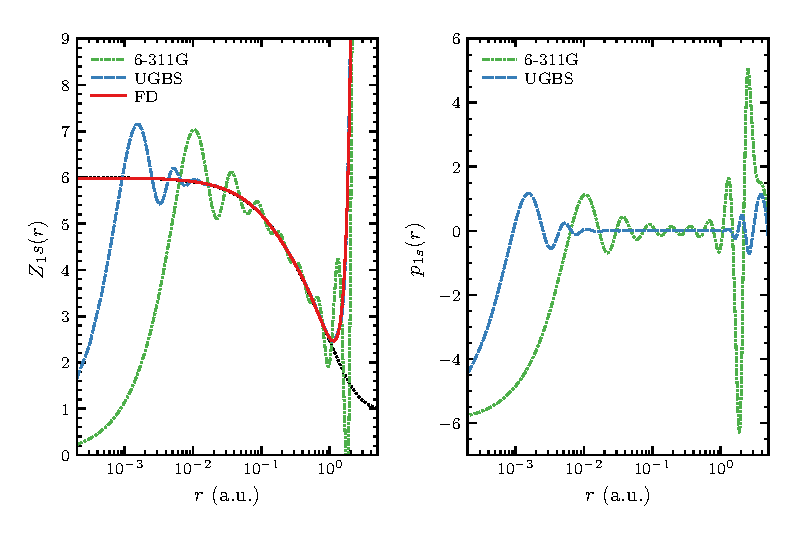
\includegraphics[width=0.9\textwidth]{dim/carbon_prof.eps}
\caption[Inversión de orbitales descritos con conjuntos de base finitos.]
{(a) Cargas efectivas invertidas del orbital $1s$ del átomo de carbón.
(b)~Perfiles de oscilación de los conjuntos de base.}
\label{fig:1sCarbon}
\end{figure}

Para ilustrar este procedimiento, se considera el orbital $1s$ del átomo 
de carbono. Primero, se resuelven las ecuaciones de Hartree--Fock usando 
el conjunto de bases \mbox{6-311G} con el código 
{\sc gamess}~\cite{Schmidt:93,Gordon:05}. Luego, aplicando la 
Ec.~(\ref{eq:Vinv}), se obtiene la carga invertida correspondiente. La 
carga resultante $Z_{1s}^{\mbox{\scriptsize 6-311G}}$ se muestra en la 
Fig.~\ref{fig:1sCarbon}(a) con una línea raya-punto. La carga tiene  
oscilaciones en toda su extensión radial, divergiendo para valores 
grandes de $r$. Se realiza el mismo cálculo con el conjunto de base 
universal gaussiano (\acs{ugbs}), que tiene un número significativamente 
mayor de funciones primitivas. La carga invertida correspondiente 
$Z_{1s}^{\mbox{\scriptsize UGBS}}$ se presenta en la figura con una línea 
discontinua. A pesar que la carga aún diverge cerca de 
$r\approx1\,$a.u., las oscilaciones ahora están circunscriptas cerca del 
núcleo. Finalmente, se resuelven las ecuaciones diferenciales de 
Hartree--Fock para el átomo de carbono usando el método de diferencias 
finitas (\acs{fd}). La carga invertida $Z_{1s}^{\mbox{\scriptsize FD}}$ 
correspondiente se exhibe con una línea sólida en la 
Fig.~\ref{fig:1sCarbon}(a). Como es de esperar, esta carga invertida no 
presenta oscilaciones, ya que no se utilizó una base para construir los 
orbitales. Sin embargo, como se vio en la Sección anterior, la carga 
diverge para $r>1\,$a.u. debido a las características 
de la teoría de Hartree--Fock. En el caso del carbono, los conjuntos de base considerados para 
calcular el orbital $1s$ fueron \mbox{6-311G} y UGBS. Los perfiles de 
oscilación correspondientes, usando la Ec.~(\ref{eq:oscillation-prof}), 
se muestran en la Fig.~\ref{fig:1sCarbon}(b). Dado que los perfiles de 
oscilación para cada conjunto de base atómico son característicos, una 
vez determinados, éstos se pueden implementar para remover las 
oscilaciones de los cálculos moleculares. 


\newpage
%%%%%%%%%%%%%%%%%%%%%%%%%%%%%%%%%%%%%%%%%%%%%%%%%%%%%%%%%%%%%%%%%%%%%%%%
\section{Resultados}
%%%%%%%%%%%%%%%%%%%%%%%%%%%%%%%%%%%%%%%%%%%%%%%%%%%%%%%%%%%%%%%%%%%%%%%%
\label{sec:dimresultados}

En esta Sección se presentan los resultados obtenidos mediante la  
implementación del método de inversión depurada para describir tres 
blancos atómicos (helio, nitrógeno y neón) y sistema molecular (metano). 
El DIM se combina con la primera aproximación de Born para describir la 
ionización por impacto de protones y fotones en estos blancos 
multielectrónicos. Las secciones eficaces de ionización predichas por el 
modelo DIM-FBA se examinan mediante comparación con los datos 
experimentales disponibles.

%%%%%%%%%%%%%%%%%%%%%%%%%%%%%%%%%%%%%%%%%%%%%%%%%%%%%%%%%%%%%%%%%%%%%%%%
\subsection{Estructura electrónica de blancos}
%%%%%%%%%%%%%%%%%%%%%%%%%%%%%%%%%%%%%%%%%%%%%%%%%%%%%%%%%%%%%%%%%%%%%%%%
\label{subsec:dimtarget}

Los orbitales $u_{nl}^{\mathrm{HF}}$ y energías 
$\varepsilon^{\mathrm{HF}}$ de Hartree--Fock que implementamos en la 
Ec.~(\ref{eq:Vinv}) se calculan usando los códigos {\sc hf} de C. F. 
Fischer~\cite{FroeseFischer:97}, y {\sc nrhf} de W. 
Johnson~\cite{Johnson:07}). 
Un aspecto importante en la optimización del potencial está dado por la 
autoconsistencia de los códigos numéricos implementados para el cálculo 
de las soluciones a ser invertidas. Para tal fin, se estudiaron los 
códigos de Hartree--Fock~\cite{FroeseFischer:97,Johnson:07} y se 
implementaron las grillas numéricas específicas de cada código, 
incluyendo los mismos métodos para el cálculo de derivadas. 


%%%%%%%%%%%%%%%%%%%%%%%%%%%%%%%%%%%%%%%%%%%%%%%%%%%%%%%%%%%%%%%%%%%%%%%%
\subsubsection*{Helio}
%%%%%%%%%%%%%%%%%%%%%%%%%%%%%%%%%%%%%%%%%%%%%%%%%%%%%%%%%%%%%%%%%%%%%%%%

En primer lugar, se muestran los resultados obtenidos de implementar
el método de inversión depurada en el átomo de helio en su estado
fundamental. Dado que el orbital $1s$ no tiene nodos y que éste 
decae exponencialmente con la energía del orbital HOMO, la inversión 
directa de este orbital no presenta ninguno de los defectos numéricos
presentados en la Sección~\ref{subsec:invHF}. Además, la simplicidad 
del átomo de helio nos permite ajustar la carga invertida con un número 
reducido de parámetros. La carga invertida $Z_{1s}^{\mathrm{HF}}$ y la
carga invertida depurada $Z_{1s}^{\mathrm{DIM}}$ se muestran en la 
Fig.~\ref{fig:Hepots}(a) con línea discontinua y sólida, 
respectivamente. La carga DIM descrita por la Ec.~(\ref{eq:atomzDIM}), 
se optimiza con sólo tres parámetros, los cuales se dan en la 
Tabla~\ref{tab:params-atoms}. 

\begin{figure}[t]
\centering
\includegraphics[width=0.9\textwidth]{figures/dim/Hepots.eps}
\caption[Cargas efectivas y potencial de intercambio DIM de He.]
{(a) Cargas efectivas $1s$ del He ($^1$S) obtenidas mediante inversión 
directa (línea discontinua) e inversión depurada (línea sólida). 
(b) Potencial de intercambio DIM (línea sólida) y OPM (línea punteada).}
\label{fig:Hepots}
\end{figure}

Para verificar la calidad de la estructura atómica dada por el potencial 
DIM, en la Tabla~\ref{tab:results-atoms} se presenta una comparación 
entre los valores de energías total, orbital y radios medios obtenidos 
utilizando el método de inversión depurada (fila superior) con sus 
correspondientes valores de Hartree--Fock (fila inferior). El potencial 
$V_{1s}^{\mathrm{ DIM}}$ es capaz de producir un valor de energía total, 
dada por la Ec.~\ref{eq:Etotal}, en un $0.003\%$. La energía orbital 
$1s$ coincide con la energía de HF en 6 cifras significativas, mientras 
que los valores medios de $u_{1s}^{\mathrm{DIM}}$ también muestran una 
excelente concordancia, tanto para la región cercana al origen, 
$\langle 1/r\rangle$, como en la región lejana, $\langle r\rangle$.

El potencial de intercambio DIM del átomo de helio, dado por la 
Ec.~\ref{eq:exchange-potential}, se muestra en la 
Fig.~\ref{fig:Hepots}(b). En la figura también se muestran los valores 
OPM, que se obtienen a partir del código \textsc{atomopm} de 
Talman~\cite{Talman:89}, coincide con $V_{1s}^{\mathrm{DIMx}$ en todo 
el rango de $r$. Las energías total y orbital de intercambio, dadas por 
la Ec.~\ref{eq:exchange-energy}, del estado fundamental del helio se 
presentan en la Tabla~\ref{tab:exchange-atoms} y se comparan con el
valor de intercambio exacto de Hartree--Fock (EAHF, por sus siglas en 
inglés) dado por Becke~\cite{Becke:14}.

%%%%%%%%%%%%%%%%%%%%%%%%%%%%%%%%%%%%%%%%%%%%%%%%%%%%%%%%%%%%%%%%%%%%%%%%
\subsubsection*{Nitrógeno}
%%%%%%%%%%%%%%%%%%%%%%%%%%%%%%%%%%%%%%%%%%%%%%%%%%%%%%%%%%%%%%%%%%%%%%%%

Los excelentes resultados obtenidos a partir de la implementación de DIM 
en el átomo de helio pueden atribuirse a la simplicidad del orbital y su 
simetría esférica. Para evaluar la destreza del método de inversión 
depurada para describir blancos con más electrones y de capa abierta, 
se considera ahora el átomo de nitrógeno. 

\begin{figure}[t]
\centering
\includegraphics[width=0.9\textwidth]{figures/dim/N4S_DIM.eps}
\caption[Cargas efectivas DIM de N.]
{Cargas efectivas $1s$, $2s$ y $2p$ del término $^4$S de N obtenidas 
mediante inversión directa (líneas discontinuas) e inversión depurada 
(líneas sólidas).}
\label{fig:Nzeff}
\end{figure}

\begin{figure}[t]
\centering
\includegraphics[width=0.9\textwidth]{figures/dim/N_Vx.eps}
\caption[Potenciales de intercambio DIM de N.]
{Potenciales de intercambio DIM de los términos $^4$S (línea sólida), 
$^2$D (línea discontinua) y $^2$P (línea punto-raya), y valores OPM 
(línea punteada) de N.}
\label{fig:NVx}
\end{figure}

La configuración más baja del nitrógeno $2p^3$ da lugar a tres términos 
diferentes: $^4$S, $^2$D, $^2$P. Cada uno de estos términos está 
descrito por una densidad electrónica diferente. 
En la Fig.~\ref{fig:Nzeff} se muestran las cargas de los orbitales $1s$, 
$2s$ y $2p$ obtenidas a partir de la inversión directa (líneas 
discontinuas) y el método de inversión depurada (líneas continuas) del 
término de energía más bajo de N. Como se vió en la  
Sección~\ref{subsec:invHF}, la inversión del orbital 
$u_{1s}^{\mathrm{HF}}$ diverge en la región asintótica debido a la 
Ec.~\ref{eq:asintoticoVHF}, mientras que el nodo genuino del orbital 
$2s$, en $r\approx 0.32$~a.u., es traducido por la inversión directa 
como un polo a la carga. 

La implementación del método de inversión depurada permite ajustar 
analíticamente la carga invertida en el mayor rango posible. Luego de 
una optimización cuidadosa del blanco, se obtienen los parámetros de las 
cargas DIM correspondientes a los términos $^4$S, $^2$D y $^2$P, que se 
dan en la Tabla~\ref{tab:params-atoms}. Las soluciones que se obtienen 
de la implementación de los potenciales DIM de N se presentan en la 
Tabla~\ref{tab:results-atoms}. Las energías totales, orbitales y valores 
radiales medios se reproducen hasta en un $0.05\%$, $1\times 10^{-4}$ y 
$0.3$ de los valores HF, respectivamente. 

En la Fig.~\ref{fig:NVx} se muestran los potenciales de intercambio 
$1s$, $2s$ y $2p$ de los términos $^4$S (línea sólida), $^2$D (línea 
discontinua) y $^2$P (línea raya-punto) de N. Los potenciales 
$V_{nl}^{\mathrm{DIMx}$ se comparan con el potencial de intercambio OPM
de Talman (línea punteada). Los potenciales de intercambio del orbital 
$1s$ de los términos se comportan de manera similar. El potencial OPM
sigue el comportamiento de estos valores cerca del origen y 
asintóticamente. En el caso del orbital $2s$, los potenciales de 
intercambio correspondientes a cada término se comportan de manera 
diferente en el origen. Para valores $r>0.5$~a.u., los potenciales DIM
y OPM convergen. Nótese que el potencial OPM se comporta como el 
potencial $V_{2s}^{\mathrm{DIMx}$ del término $^2$D concuerda muy bien.
Los potenciales de intercambio DIM $2p$ también se comportan de manera
similar. Sin embargo, los potenciales DIM y OPM convergen sólo en la 
región asintótica. Es notable como el potencial, que no es orbital, 
tiende a seguir el comportamiento de los potenciales orbitales DIM a lo 
largo de $r$. 

Los valores de energía de intercambio orbitales y total de los términos 
$^4$S, $^2$D y $^2$P de N se muestran en la 
Tabla~\ref{tab:exchange-atoms}. La energía de intercambio orbital $1s$ 
de todos los términos son iguales, como se esperaría para un orbital de 
capa cerrada. De manera similar, las energías correspondientes al 
orbital $2s$ varían ligeramente, con una dispersión del $0.08\%$. Sin 
embargo, dado que la capa $2p$ está abierta, la energía de intercambio 
del orbital $2p$ varía significativamente en los diferentes términos, 
con una dispersión de hasta 18\%. Por otro lado, las energías de 
intercambio total, que se obtiene a partir de la 
Ec.~(\ref{eq:exchange-energy}), se comparan con los valores EAHF y 
presentan un acuerdo cercano al $0.1\%$.

%%%%%%%%%%%%%%%%%%%%%%%%%%%%%%%%%%%%%%%%%%%%%%%%%%%%%%%%%%%%%%%%%%%%%%%%
\subsubsection*{Neón}
%%%%%%%%%%%%%%%%%%%%%%%%%%%%%%%%%%%%%%%%%%%%%%%%%%%%%%%%%%%%%%%%%%%%%%%%

La implementación del DIM en neón es análoga al caso de nitrógeno. Esta
vez, la capa de valencia del átomo está llena. Los resultados de la 
optimización de los parámetros que definen las cargas efectivas, dadas 
por la Ec.~(\ref{eq:atomzDIM}), del átomo de neón se muestran en la 
Tabla~\ref{tab:params-atoms}. La comparación entre las soluciones de los 
potenciales DIM y el método de Hartree--Fock se dan en la 
Tabla~\ref{tab:results-atoms}. El acuerdo en energías orbitales es 
excelente, del orden de $1\times 10^{-5}$, mientras que DIM reproduce 
los valores medios de los orbitales HF en aproximadamente $0.1\%$. Por 
otro lado, la energía total tiene una dispersión del $0.04\%$ respecto 
a HF. Las energías de intercambio total y orbitales que se obtienen a 
partir del DIM se presentan en la Tabla~\ref{tab:exchange-atoms}. Las 
energías $E^{\mathrm{x}$ y los valores EAHF acuerdan en $0.04\%$.

%%%%%%%%%%%%%% RESULTADOS %%%%%%%%%%%%%%
\begin{table}
\begin{center}
\begin{tabularx}{\textwidth}{
>{\centering\arraybackslash}p{0.12\textwidth}
>{\centering\arraybackslash}p{0.05\textwidth}
>{\centering\arraybackslash}p{0.22\textwidth}
>{\centering\arraybackslash}p{0.22\textwidth}
>{\centering\arraybackslash}p{0.22\textwidth}}
\rowcolor{mydarkgray} 
   &       & $nl$ & $z_j$        & $\alpha_j$   \\
%%%%%%%%%%%%%%%%%%%% Helio %%%%%%%%%%%%%%%%%%%%
He & $^1$S & $1s$ &  $1.3175$ & $2.5003$  \\\rowcolor{mygray} 
   &       &      & $-0.3175$ & $5.0437$  \\ 
%%%%%%%%%%%%%%%%%% Nitrogeno %%%%%%%%%%%%%%%%%%
N  & $^4$S & $1s$ & $5.2563$ & $1.2621$  \\\rowcolor{mygray} 
   &       &      & $0.7437$ & $8.0284$  \\ 
   &       & $2s$ & $2.7136$ & $0.8947$ \\\rowcolor{mygray} 
   &       &      & $2.4528$ & $3.5127$  \\
   &       &      & $0.8336$ & $3.3865$  \\ \rowcolor{mygray} 
   &       & $2p$ & $3.6435$ & $1.2407$  \\ 
   &       &      & $2.0550$ & $5.3514$  \\\rowcolor{mygray} 
   &       &      & $0.3015$ & $0.2866$ \\
   & $^2$D & $1s$ & $5.1664$ & $1.2241$  \\\rowcolor{mygray} 
   &       &      & $0.8137$ & $7.5680$  \\ 
   &       & $2s$ & $3.7478$ & $2.8531$  \\\rowcolor{mygray} 
   &       &      & $1.8541$ & $1.0311$  \\ 
   &       &      & $0.3981$ & $0.2397$ \\\rowcolor{mygray} 
   &       & $2p$ & $4.0105$ & $1.2874$  \\ 
   &       &      & $1.8552$ & $5.7086$  \\\rowcolor{mygray} 
   &       &      & $0.1343$ & $0.2680$ \\
   & $^2$P & $1s$ & $5.1864$ & $1.2178$  \\\rowcolor{mygray} 
   &       &      & $0.8137$ & $7.5674$  \\ 
   &       & $2s$ & $3.6700$ & $3.1495$  \\\rowcolor{mygray} 
   &       &      & $1.4394$ & $0.7404$  \\ 
   &       &      & $0.8907$ & $0.8306$ \\\rowcolor{mygray} 
   &       & $2p$ & $2.3280$ & $1.4093$  \\ 
   &       &      & $1.8977$ & $1.1656$  \\\rowcolor{mygray} 
   &       &      & $1.7743$ & $5.6878$ \\
%%%%%%%%%%%%%%%%%%%%%%%%%%%%%%%%%%%%%%%%%%%%%%%
Ne & $^1$S & $1s$ & $7.3677$ & $2.4173$ \\\rowcolor{mygray} 
   &       &      & $1.3004$ & $0.1264$ \\
   &       &      & $0.3320$ & $13.1582$ \\\rowcolor{mygray} 
   &       & $2s$ & $0.2977$ & $17.9939$ \\
   &       &      & $0.6681$ & $0.0673$ \\\rowcolor{mygray} 
   &       &      & $8.0342$ & $2.4722$ \\
   &       & $2p$ & $1.3531$ & $8.5695$ \\\rowcolor{mygray} 
   &       &      & $0.3359$ & $0.4649$ \\
   &       &      & $7.3111$ & $2.0906$ \\
\end{tabularx}
\caption[Parámetros de la carga efectiva de He, N y Ne.]
{Parámetros de la carga efectiva $Z_{1s}^{\mathrm{ DIM}}$ de He ($^1$S), 
N ($^4$S, $^2$D, $^2$P) y Ne ($^1$S).}
\label{tab:params-atoms}
\end{center}
\end{table}

\begin{table}
\begin{center}
\begin{tabularx}{\textwidth}{
>{\centering\arraybackslash}p{0.07\textwidth}
>{\centering\arraybackslash}p{0.03\textwidth}
>{\centering\arraybackslash}p{0.15\textwidth}
>{\centering\arraybackslash}p{0.10\textwidth}
>{\centering\arraybackslash}p{0.15\textwidth}
>{\centering\arraybackslash}p{0.15\textwidth}
>{\centering\arraybackslash}p{0.15\textwidth}}
\rowcolor{mydarkgray} 
   & & $E$ & $nl$ & $\varepsilon_{nl}$ & $\left<r\right>_{nl}$ & $\left<1/r\right>_{nl}$ \\
He & $^1$S & $-2.8616$   & $1s$ & $-0.9180$  & $0.9273$ & $1.6873$ \\\rowcolor{mygray} 
   &       & $-2.8617$   &      & $-0.9180$  & $0.9273$ & $1.6873$ \\
N  & $^4$S & $-54.3762$  & $1s$ & $-15.6291$ & $0.2283$ & $6.6487$ \\\rowcolor{mygray} 
   &       & $-54.4009$  &      & $-15.6291$ & $0.2283$ & $6.6532$ \\
   &       &             & $2s$ & $-0.9453$  & $1.3345$ & $1.0804$ \\\rowcolor{mygray} 
   &       &             &      & $-0.9453$  & $1.3323$ & $1.0782$ \\
   &       &             & $2p$ & $-0.5676$  & $1.4127$ & $0.9550$ \\\rowcolor{mygray} 
   &       &             &      & $-0.5676$  & $1.4096$ & $0.9577$ \\
   & $^2$D & $-54.2756$  & $1s$ & $-15.6664$ & $0.2283$ & $6.6493$ \\\rowcolor{mygray} 
   &       & $-54.2962$  &      & $-15.6664$ & $0.2283$ & $6.6539$ \\
   &       &             & $2s$ & $-0.9637$  & $1.3292$ & $1.0874$ \\\rowcolor{mygray} 
   &       &             &      & $-0.9637$  & $1.3263$ & $1.0832$ \\
   &       &             & $2p$ & $-0.5087$  & $1.4488$ & $0.9388$ \\\rowcolor{mygray} 
   &       &             &      & $-0.5087$  & $1.4466$ & $0.9421$ \\
   & $^2$P & $-54.2086$  & $1s$ & $-15.6916$ & $0.2282$ & $6.6504$ \\\rowcolor{mygray} 
   &       & $-54.2281$  &      & $-15.6916$ & $0.2282$ & $6.6543$ \\
   &       &             & $2s$ & $-0.9763$  & $1.3256$ & $1.0871$ \\\rowcolor{mygray} 
   &       &             &      & $-0.9763$  & $1.3223$ & $1.0866$ \\
   &       &             & $2p$ & $-0.4713$  & $1.4718$ & $0.9298$ \\\rowcolor{mygray} 
   &       &             &      & $-0.4713$  & $1.4730$ & $0.9316$ \\
Ne & $^1$S & $-128.4978$ & $1s$ & $-32.7725$ & $0.1575$ & $9.6215$ \\\rowcolor{mygray} 
   &       & $-128.5475$ &      & $-32.7724$ & $0.1576$ & $9.6181$ \\
   &       &             & $2s$ & $-1.9304$  & $0.8913$ & $1.6408$ \\\rowcolor{mygray} 
   &       &             &      & $-1.9304$  & $0.8921$ & $1.6326$ \\  
   &       &             & $2p$ & $-0.8504$  & $0.9678$ & $1.4303$ \\\rowcolor{mygray} 
   &       &             &      & $-0.8504$  & $0.9653$ & $1.4354$ \\
\end{tabularx}
\caption[Energías y radios medios de He, N y Ne.]
{Energías totales, energías orbitales y radios medios de He ($^1$S), 
N ($^4$S, $^2$D, $^2$P) y Ne ($^1$S) obtenidos con el método de 
inversión depurada (filas superiores) y con el método de HF (filas 
inferiores).}
\label{tab:results-atoms}
\end{center}
\end{table}

\begin{table}
\begin{center}
\begin{tabularx}{\textwidth}{
>{\centering\arraybackslash}p{0.07\textwidth}
>{\centering\arraybackslash}p{0.03\textwidth}
>{\centering\arraybackslash}p{0.14\textwidth}
>{\centering\arraybackslash}p{0.14\textwidth}
>{\centering\arraybackslash}p{0.14\textwidth}
>{\centering\arraybackslash}p{0.14\textwidth}
>{\centering\arraybackslash}p{0.14\textwidth}}
\rowcolor{mydarkgray} 
   &      & $1s$     & $2s$     & $3s$     & Total    & EAHF~\cite{Becke:14} \\
He & $^1$S & $-0.5129$ &           &           & $-1.0258$ & $-1.026$ \\\rowcolor{mygray} 
N  & $^4$S & $-2.1175$ & $-0.4776$ & $-0.4711$ & $-6.6034$ & $-6.596$ \\
   & $^2$D & $-2.1175$ & $-0.4777$ & $-0.4262$ & $-6.4688$ & \\\rowcolor{mygray} 
   & $^2$P & $-2.1175$ & $-0.4780$ & $-0.3973$ & $-6.3827$ & \\
Ne & $^1$S & $-3.1106$ & $-0.8620$ & $-0.6938$ & $-12.1080$ & $-12.105$ \\\rowcolor{mygray} 
\end{tabularx}
\caption[Energías de intercambio total y orbitales de He, N y Ne.]
{Energías de intercambio total y orbitales DIM de He ($^1$S), N ($^4$S, 
$^2$D, $^2$P) y Ne ($^1$S).}
\label{tab:exchange-atoms}
\end{center}
\end{table}

\newpage
%%%%%%%%%%%%%%%%%%%%%%%%%%%%%%%%%%%%%%%%%%%%%%%%%%%%%%%%%%%%%%%%%%%%%%%%
\subsubsection*{Metano}
%%%%%%%%%%%%%%%%%%%%%%%%%%%%%%%%%%%%%%%%%%%%%%%%%%%%%%%%%%%%%%%%%%%%%%%%

El método de inversión depurada para sistemas moleculares se aplica a 
la molécula de metano. Este hidruro es altamente simétrico y, por lo 
tanto, puede ser descrito por un potencial angular 
promediado~\cite{Granados:16}. 

\begin{figure}[t]
\centering
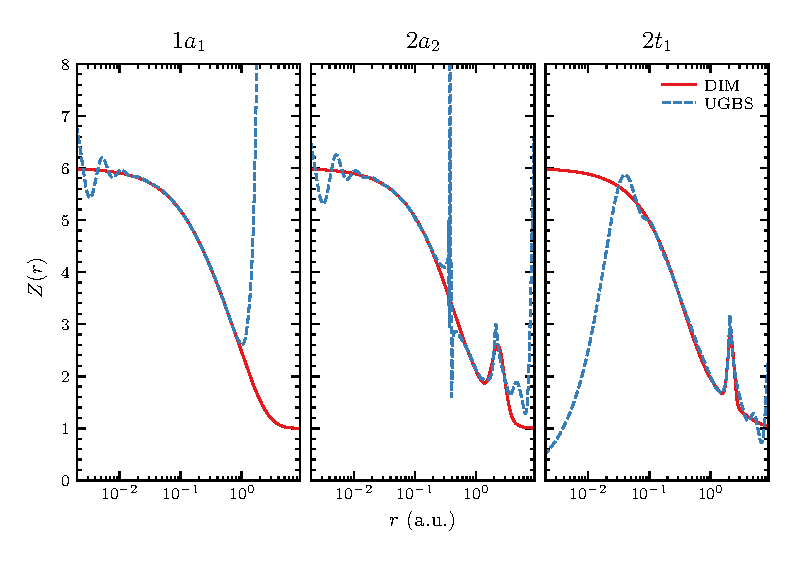
\includegraphics[width=0.9\textwidth]{figures/dim/ch4_dim.eps}
\caption[Cargas invertidas y depuradas de metano.]
{Cargas efectivas de CH$_4$ de los orbitales moleculares $1a_1$, $2a_2$ 
y $2t_1$ obtenidas a partir del conjunto de base UGBS; inversión directa 
(líneas discontinuas) e inversión depurada (líneas sólidas).}
\label{fig:ch4zeff}
\end{figure}

% ver si incluir una frase sobre la expansión de un centro de los orbitales moleculares multicentricos
Los orbitales moleculares HF de CH$_4$ se calculan usando los conjuntos 
de bases UGBS del carbono y el hidrógeno. Estas bases sólo consideran 
momentos angulares hasta $L=1$. El cálculo de estructura electrónica de 
metano con estos conjuntos de base deberían incluir funciones de 
polarización (por lo menos hasta las funciones $d$), con el fin de 
incrementar la precisión de las energías moleculares~\cite{Rothenberg:71,
Hariharan:72}. Sin embargo, para aislar los efectos de la base, los 
cálculos de perfiles de oscilación descritos en la 
Sección~\ref{sec:dimmoleculas} y los orbitales moleculares se realizan 
en el mismo esquema. Las cargas obtenidas mediante la inversión directa 
de estos orbitales se muestran en la Fig.~\ref{fig:ch4zeff} con líneas 
discontinuas. Dado que los orbitales moleculares están escritos por 
combinaciones lineales de orbitales atómicos del carbono y el hidrógeno, 
las oscilaciones de las cargas invertidas se deben al número finito de 
funciones primitivas en el conjunto de base de cada átomo. Para remover 
estas oscilaciones, se deben determinar los perfiles de oscilación 
producidas por la base de los átomos constituyentes. Se emplea la 
Ec.~(\ref{eq:oscillation-prof}) para determinar los perfiles 
$p_{1s}^{\mbox{\scriptsize UGBS}}$, $p_{2s}^{\mbox{\scriptsize UGBS}}$ y 
$p_{2p}^{\mbox{\scriptsize UGBS}}$ del carbono. Así, se puden remover 
los perfiles $p_{nl}^{\mbox{\scriptsize UGBS}}$ de las correspondientes 
cargas invertidas $Z_{nl}^{\mbox{\scriptsize UGBS}}$ del metano. Las 
oscilaciones se remueven completamente para todos los orbitales excepto 
el $2a_2$, que presenta pequeñas fluctuaciones residuales debido a la 
base del hidrógeno. Ya que estas ondulaciones son mínimas y se ubican 
cerca del núcleo, éstas pueden ser despreciadas y se procede a 
implementar el método de depuración descrito en la 
Sección~\ref{sec:dimmoleculas}. 

Los parámetros optimizados de las cargas moleculares DIM, dadas por la 
Ec.~(\ref{eq:molzDIM}), se presentan en la Tabla~\ref{tab:ch4parameters}. 
Las cargas correspondientes se muestran en la Fig.~\ref{fig:ch4zeff} con 
líneas sólidas. En este caso, para la construcción de función de 
costo~(\ref{eq:fncosto-dim}) que se miniza considera los valores de 
energía y radios medios de los MOs dados por Moccia~\cite{Moccia:69}. 
las energías orbitales reproducen las originales hasta la cuarta cifra 
significativa y se dan en la Tabla~\ref{tab:ch4parameters}. Por otro 
lado, los radios medios $\langle r\rangle$ y $\langle 1/r\rangle$ 
obtenidos con los potenciales moleculares DIM están dentro del $1\%$ 
de los valores de Moccia.

\begin{table}[t]
\centering
\begin{tabular}{
>{\centering\arraybackslash}p{0.13\textwidth}
>{\centering\arraybackslash}p{0.13\textwidth}
>{\centering\arraybackslash}p{0.13\textwidth}
>{\centering\arraybackslash}p{0.13\textwidth}
>{\centering\arraybackslash}p{0.13\textwidth}
>{\centering\arraybackslash}p{0.13\textwidth}}
\rowcolor{mydarkgray} 
   $nl$ & $E$        & $z$        & $\alpha$   & $\beta$ & $\gamma$ \\
$1a_1$  & $-11.1949$ & $1.925280$ & $0.641982$ & & \\
\rowcolor{mygray} 
        &            & $0.953120$ & $5.571510$ & & \\
        &            & $2.121600$ & $1.500440$ & & \\
\rowcolor{mygray} 
$2a_2$  & $-0.9204$  & $2.912200$ & $3.149990$ & & \\
        &            & $2.087800$ & $0.771371$ & & \\
\rowcolor{mygray} 
        &            & $1.23640$  &            & $2.329570$ & $0.053420$ \\
$2t_1$  & $-0.5042$  & $0.901953$ & $2.895140$ & & \\
\rowcolor{mygray} 
        &            & $1.112030$ & $0.388649$ & & \\
        &            & $2.986017$ & $2.931210$ & & \\
\rowcolor{mygray} 
        &            & $1.301820$ &            & $2.169850$ & $0.012616$ \\ 
\end{tabular}
\caption[Energías y parámetros de ajuste de cargas efectivas de metano.]
{Energías orbitales moleculares y parámetros de ajuste de cargas 
efectivas de metano.}
\label{tab:ch4parameters}
\end{table}

%%%%%%%%%%%%%%%%%%%%%%%%%%%%%%%%%%%%%%%%%%%%%%%%%%%%%%%%%%%%%%%%%%%%%%%%
\subsection{Procesos colisionales simples}
%%%%%%%%%%%%%%%%%%%%%%%%%%%%%%%%%%%%%%%%%%%%%%%%%%%%%%%%%%%%%%%%%%%%%%%%
\label{subsec:procol}

En esta Sección se analiza la respuesta de los potenciales efectivos 
DIM obtenidos en la Sección~\ref{subsec:dimtarget} mediante el método 
de inversión depurada para helio, nitrógeno, neón y metano.
En los blancos moleculares, la orientación molecular es importante para 
determinar la sección eficaz en un proceso colisional. Sin embargo, en 
sistemas gasesosos, las moléculas tienen orientaciones aleatorias que no 
están predefinidas en el experimento. Por lo tanto, la descripción 
promediada esféricamente de los sistemas moleculares asumida por el 
potencial DIM está en concordancia con la configuración del blanco.
Los procesos colisionales que se examinan en esta Sección se describen a 
primer orden empleando la primera aproximación de Born (FBA). 
La combinación de la descripción del blanco mediante el potencial 
efectivo DIM y el modelado de la fotoionización a primer orden se 
denomina como ionización DIM-FBA. 

%%%%%%%%%%%%%%%%%%%%%%%%%%%%%%%%%%%%%%%%%%%%%%%%%%%%%%%%%%%%%%%%%%%%%%%%
\subsubsection{Fotoionización}
%%%%%%%%%%%%%%%%%%%%%%%%%%%%%%%%%%%%%%%%%%%%%%%%%%%%%%%%%%%%%%%%%%%%%%%%
\label{subsec:foto}

Las secciones eficaces de ionización simple por impacto de fotón según 
el modelo DIM-FBA para helio, nitrógeno, neón y metano se muestran en 
la Fig.~\ref{fig:photoDIM} con líneas sólidas. Los resultados teóricos 
DIM-FBA para helio y nitrógeno coinciden de manera excelente con los 
valores experimentales (símbolos)~\cite{Samson:90,Henke:93,Stolte:16} a 
bajas, medias y altas energías del fotón incidente. En el caso del átomo 
de neón, algunas discrepancias con las mediciones (símbolos) 
\cite{Henke:93,Samson:02} empiezan a surgir a energías bajas e 
intermedias del projectil. Este comportamiento sugiere la necesidad de 
incluir en la descripción de la fotoionización correcciones de mayor 
orden que incluyan efectos de múltiples cuerpos que puedan ser 
relevantes, tales como la relajación de los orbitales debido a la 
creación de un hueco electrónico, respuestas colectivas de electrones 
de capas internas~\cite{Ederer:64} y efectos de correlación.

\begin{figure}
\centering
\includegraphics[width=0.92\textwidth]{dim/fotoDIM-part1.eps} 

\vspace{-1.15cm}
\includegraphics[width=0.92\textwidth]{dim/fotoDIM-part2.eps}
\caption[Fotoionización de He, N, Ne y CH$_4$.]
{Sección eficaz total de fotoionización de un electrón de He~$^1$S, 
N~$^4$S, Ne~$^1$S y CH$_4$. Curvas: cálculos teóricos DIM-FBA. Símbolos: 
datos experimentales~\cite{Samson:90,Henke:93,Stolte:16,Samson:02,
Lukirskii:64,Henke:82,Samson:89}.}
\label{fig:photoDIM}
\end{figure}

La predicción del modelo DIM-FBA para la sección eficaz total de 
fotonización de CH$_4$ se encuentra en buen acuerdo con valores 
experimentales en el rango de altas energías y cerca del umbral. La 
curva entre aproximadamente 15 y 300 eV muestra la fotoionización de la 
capa eterna $n=2$, mientras que la discontinuidad en $0.3$~keV 
corresponde al umbral del orbital molecular $1a_1$. Para fotoenergías 
bajas e intermedias, el acuerdo entre las predicciones DIM-FBA y los 
datos experimentales~\cite{Lukirskii:64,Henke:82,Samson:89} no es bueno. 
Fenónemos tales como la relajación de los orbitales moleculares, 
posibles contribuciones colectivas y efectos de correlación deben ser  
considerados en futuros cálculos. Por otro lado, para la fotoionización 
de un electrón perteneciente al orbital interno $1a_1$, estos efectos no 
son tan signficativos, y se tiene buen acuerdo con los valores 
experimentales disponibles. 

%=======================================================================
\subsubsection{Ionización por impacto de iones}
\label{subsec:dimion}

\begin{figure}
\centering
\includegraphics[width=0.9\textwidth]{figures/dim/ionDIM.eps}
\caption[Ionización por impacto de protón de N y CH$_4$.]
{Sección eficaz total de ionización de un electrón por impacto de protón 
de N~$^4$S y CH$_4$. Línea sólida: cálculos teóricos DIM-FBA. 
Símbolos: datos experimentales de ionización por impacto de 
protón~\cite{Rudd:83,Rudd:85} y electrón~\cite{Brook:78} con conversión 
de equivelocidad.}
\label{fig:iondim}
\end{figure}

Los resultados de ionización por impacto de protón en N~$^4$S y CH$_4$, 
en el marco del modelo DIM-FBA, se muestra en la Fig.~\ref{fig:iondim}. 
El acuerdo entre las predicciones teóricas y las datos experimentales es 
muy bueno en la región de altas energías, donde tiene validez la primera 
aproximación de Born. En el caso de nitrógeno, incluimos también datos 
experimentales de ionización por impacto de electrón. Para valores de 
energía mayores a 400~keV, se espera que la sección eficaz de ambos 
proyectiles coincida. 

%=======================================================================
\section{Conclusiones}
\label{conclusion}

En este Capítulo se desarrolló el método de inversión depurada (DIM) 
para obtener potenciales efectivos que permitan describir la estructura 
electrónica de blancos atómicos y moleculares de manera precisa. La 
disponibilidad de estos potenciales permite conocer los estados 
iniciales y finales del blanco en una colisión de manera directa. 

Los potenciales DIM se obtienen a partir de la inversión de ecuaciones 
de un electrón con soluciones de Hartree--Fock. Los potenciales 
resultantes presentan defectos numéricos (polos y divergencias), los 
cuales son examinados en detalle. Se encuentra que los defectos están 
dados por características de la teoría de Hartree--Fock no compatibles
con la inversión. Los polos se deben a nodos genuinos de los orbitales 
HF que no son puntos de inflexión. Si bien esta característica de los 
orbitales no es explícita en la teoría, la obtención de potenciales sin 
polos así lo requiere. Las divergencias asintóticas del potencial se 
deben al coeficiente del decaimiento exponencial de los orbitales HF. 
La teoría de HF establece que éstos decaen con la energía del HOMO. Sin 
embargo, la obtención de potenciales con correcto comportamiento 
asintótico mediante el esquema de inversión requiere que cada orbital 
decaiga con la energía del dicho orbital. También se encontraron 
oscilaciones en los orbitales de las capas internas de átomos con carga 
nuclear $Z\ge 12$, que dan lugar a nodos espurios. Estas oscilaciones 
parecen surgir debido al término de intercambio a grandes distancias. 
Para tratar los defectos encontrados en la inversión, se desarrolló el 
método de depuración, que consiste en ajustar las cargas invertidas, en 
regiones sin polos ni divergencias, mediante una expresión analítica. 
Los parámetros que definen esta expresión son optimizados cuidadosamente 
hasta reproducir las soluciones iniciales.

El método de inversión depurada para átomos fue extendido para 
moléculas. Debido a que los orbitales moleculares se expresan a partir 
de conjuntos de base finitas, las soluciones presentan ondulaciones casi 
imperceptiles. La implementación de la inversión traduce estas pequeñas 
fluctuaciones como grandes oscilaciones en la carga molecular. Debido a 
esto, se requieren pasos adicionales en el método de depuración, los 
cuales incluyen la determinación de perfiles de oscilación de los 
conjuntos de base atómicas utilizadas en el cálculo molecular. 

Dado que la teoría de Hartree--Fock contiene el término de intercambio
de forma exacta, a partir de los potenciales DIM, se definió una 
expresión que permite determinar potenciales de intercambio orbitales 
``exactos'' de manera simple. A su vez, estos potenciales se emplean 
para definir energías de intercambio orbitales y totales.

Se implementó el método DIM para obtener potenciales efectivos y de 
intercambio que reproducen las soluciones de HF de forma precisa en tres 
blancos atómicos: helio, nitrógeno y neón. Además, se empleó el método 
DIM extendido a moléculas para describir la molécula de metano. Las 
soluciones que se obtienen de estos potenciales reproducen los valores
originales con gran precisión. 

La efectividad del DIM para describir la estructura de blancos en una 
colisión fue examinado a partir de la primera aproximación de Born. Los 
potenciales de He, N, Ne y CH$_4$ se implementaron para calcular, en 
conjunción con la FBA, secciones eficaces de ionización por el impacto 
de protones y fotones. En términos generales, ambos procesos se 
reproducen con buena concordancia los datos experimentales disponibles. 
Las discrepancias principales se atribuyen al hecho de que el modelo 
teórico sólo considera el primer orden perturbativo. Será necesario 
implementar métodos perturbativos con mayor orden de aproximación para 
examinar la validez del método DIM en la región de energías intermedias.


%%%%%%%%%%%%%%%%%%%%%%%%%%%%%%%%%%%%%%%%%%%%%%%%%%%%%%%%%%%%%%%%%%%%%%%%
\section{Discusión: DIM como instancia superadora de HF?}
%%%%%%%%%%%%%%%%%%%%%%%%%%%%%%%%%%%%%%%%%%%%%%%%%%%%%%%%%%%%%%%%%%%%%%%%
\label{sec:discusion}

%%% Fallas
%%% Nodos que no son puntos de inflexión  -> Derivada 2da
%%% Nodos que son espurio (no localidad) -> Fischer
%%% Divergencia a grandes r               -> Hartree

% Defectos: 
% Los defectos de las cargas invertidas surgen del propio método de Hartree--Fock; los nodos genuinos no son estrictamente puntos de  inflexión, el decaimiento exponencial de los orbitales sigue el comportamiento orbitales tipo Hartree, mientras que el método autoconsistente conduce a la aparición de nodos espurios.

En general, las cargas resultantes de la inversión de los orbitales HF 
tienen asociadas alguno de estos defectos. A partir de dos ejemplos, 
se examina cada uno de ellos y su transfondo téorico a través un 
experimento numérico. Sin embargo, el análisis se puede generalizar 
para los orbitales HF de cualquier átomo no relativista.

%%%%%%%%%%%%%%%%%%%%%%%%%%%%%%%%%%%%%%%%%%%%%%%%%%%%%%%%%%%%%%%%%%%%%%%%
\subsubsection*{Nodos genuinos}
%%%%%%%%%%%%%%%%%%%%%%%%%%%%%%%%%%%%%%%%%%%%%%%%%%%%%%%%%%%%%%%%%%%%%%%%

En la Fig.~\ref{fig:example2sMg} se muestra la función 
$u_{2s}^{\mathrm{HF}}$ del Mg y su derivada segunda numérica (escalada 
por un factor). Las dos raices de $u_{2s}^{\mathrm{HF}}''$ son puntos de 
inflexión de $u_{2s}^{\mathrm{HF}}$ y se corresponden a (1)~el nodo 
genuino y (2)~el punto de inflexión clásico. A primera vista, el nodo 
genuino y el primer punto de inflexión parecen coincidir. Sin embargo, 
una inspección más cercana (ver recuadro) muestra que ese no es el caso. 
Definiendo $\Delta r$ como la distancia entre el nodo del orbital y la 
primera raiz de su derivada segunda, se encuentra una pequeña distancia 
$\Delta r=1\times 10^{-3}$~a.u. entre las primeras raices de ambas 
funciones. Si bien no existe ninguna restricción en la teoría que fuerce 
a los nodos genuinos de HF a ser también puntos de inflexión, este 
fenómeno es sistemático en todos los orbitales HF con nodos de los 
átomos con $Z\ge 12$.

\begin{figure}
\vspace{-0.4cm}
\centering
\includegraphics[width=0.85\textwidth]{dim/example_2sMg.eps} 
\vspace{-0.45cm}
\caption[Orbital radial y su derivada segunda.]
{Orbital radial $u_{2s}^{\mathrm{HF}}$ del estado fundamental de Mg y su 
derivada segunda escalada.}
\label{fig:example2sMg}
%\end{figure}

\vspace{0.4cm}
%\begin{figure}
%\centering
\includegraphics[width=0.85\textwidth]{dim/dr_2sMg.eps} 
\vspace{-0.45cm}
\caption[Dependecia de $\Delta r$ del orden de aproximación numérica.]
{Dependecia de $\Delta r$ del orden de aproximación numérica en el 
orbital $2s$ del átomo de potasio. (a) Primer orden y 200 puntos, (b) 
400 puntos; (c) octavo orden y 1000 puntos.}
\label{fig:dr2sMg}
\end{figure}

Estos hallazgos permiten suponer que la cercanía entre los nodos 
genuinos de los orbitales y las correspondientes raices de su segunda 
derivada no es casual, y que los nodos genuinos en la teoría de 
Hartree--Fock deben ser puntos de inflexión. El experimento numérico 
que se diseña para indagar esta hipótesis consiste en realizar varias 
aproximaciones con mejoras sucesivas en su precisión, examinando el 
comportamiento del valor $\Delta r$ resultante. La calidad de los 
métodos numéricos usados para resolver las ecuaciones de HF se evalúan 
variando el orden de precisión de los algoritmos y la densidad de puntos 
de las grillas numéricas. En este experimento se utiliza el método 
lineal de pasos múltiples de Adams--Moulton para las ecuaciones 
diferenciales y el método de diferenciación Lagrangiana para las 
derivadas. La metodología propuesta se implementa modificando el código 
\textsc{nrhf} de Johnson~\cite{Johnson:07}, que usa aproximaciones de 
octavo orden por defecto. %No obstante, los mismos resultados y 
%conclusiones se obtienen con el código~\textsc{hf} de 
%Fischer~\cite{FroeseFischer:97}.

La Fig.~\ref{fig:dr2sMg} muestra $u_{2s}^{\mathrm{HF}}$ de Mg (línea 
sólida) y su segunda derivada numérica (línea discontinua) en las 
proximidades del nodo implementando tres grados de aproximación 
distintos en los métodos numéricos. Los cálculos menos precisos se 
muestran en la Fig.~\ref{fig:dr2sMg}(a), donde se implementa el primer 
orden de los algoritmos numéricos y una grilla numérica de 200 puntos 
(mínimo valor necesario para obtener convergencia), resultando en 
$\Delta r=8\times 10^{-3}$~a.u.. Aumentando el número de puntos a 400, 
este valor se reduce a $\Delta r=4\times 10^{-3}$~a.u., como se muestra 
en la Fig.~\ref{fig:dr2sMg}(b). Por último, se incrementa el número de 
puntos a 1000 y se usa el máximo orden de aproximación de los 
algoritmos. La Fig.~\ref{fig:dr2sMg}(c) muestra el mejor resultado 
posible, donde $\Delta r=1\times 10^{-3}$~a.u.. Aún considerando un 
número mayor de puntos en la grilla numérica, los resultados no varían. 
Se realizó un cálculo adicional usando el método del potencial efectivo 
optimizado (\acs{oep}) desarrollado por Talman~\cite{Sharp:53,Talman:76,
Talman:89}. La Fig.~\ref{fig:dr2sMg}(c) muestra el orbital 
$u_{2s}^{\mathrm{OEP}}$ de Mg cerca del nodo con una línea raya-punto. 
Debido al caracter local del potencial, su segunda derivada 
$u_{2s}^{\mathrm{OEP}}''$ (línea punto-raya-punto) es estrictamente cero 
en el nodo. 

Es posible que la no localidad del método de Hartree--Fock sea 
responsable de que los nodos genuinos en los orbitales no sean puntos de 
inflexión. Una exploración más en detalle, con mayores órdenes de 
aproximación en los métodos numéricos, será necesaria para descartar 
esta hipótesis. La excelente reproducción de los orbitales HF mediante 
el potencial local OEP parece sugerir que esta premisa es correcta. De 
ser el caso, se podría agregar una restricción adicional al 
procedimiento variacional autoconsistente de Hartree--Fock. En 
definitiva, el cumplimiento de esta restricción aseguraría un potencial 
local, en principio, sin polos.

%%%%%%%%%%%%%%%%%%%%%%%%%%%%%%%%%%%%%%%%%%%%%%%%%%%%%%%%%%%%%%%%%%%%%%%%
\subsubsection*{Decaimiento exponencial}
%%%%%%%%%%%%%%%%%%%%%%%%%%%%%%%%%%%%%%%%%%%%%%%%%%%%%%%%%%%%%%%%%%%%%%%%

Los orbitales de los electrones ligados decaen exponencialmente para 
distancias mayores al punto de retorno clásico. A grandes distancias 
$r$, el decaimiento asintótico de la parte radial de los orbitales HF 
está determinado por la energía del orbital molecular de mayor ocupación 
(\acs{homo}) $\varepsilon_{\mathrm{HOMO}}^{\mathrm{HF}}$ 
\cite{Handy:69,Handler:80,Ishida:92}},
\begin{equation}
\lim_{r \rightarrow \infty} u_{nl}^{\mathrm{HF}}(r) =  
\exp(- \sqrt{- 2 \varepsilon_{\mathrm{HOMO}}^{\mathrm{HF}} } r )  \, .
\label{eq:rHF}
\end{equation}
Por otro lado, los orbitales que corresponden a potenciales esféricos 
tienen un decaimiento asintótico de tipo Hartree~\cite{Casida:89},
\begin{equation}
\lim_{r \rightarrow \infty} u_{nl}^{\mathrm{DIM}}(r) =  
\exp(- \sqrt{- 2 \varepsilon_{nl}^{\mathrm{HF}} } r ) \,.
\label{eq:rHlike}
\end{equation}
El término ``tipo-Hartree'' puede resultar confuso ya que la energía 
del orbital $\varepsilon_{nl}^{\mathrm{HF}}$ se corresponde a valores 
donde se ha considerado el término de intercambio. El comportamiento 
asintótico de los orbitales HF se puede examinar en detalle a través de 
la derivada logaritmica de los orbitales radiales, 
\begin{equation}
L_{nl}(r) \equiv r \frac{d \log{u_{nl}}}{d r}\,,
\label{eq:Lnl}
\end{equation}
que se comporta de forma lineal para funciones $u_{nl}$ que decaen 
exponencialmente. 

\begin{figure}[t]
\centering
\includegraphics[width=0.9\textwidth]{dim/Lns_K.eps} 
\caption[Comportamiento asintótico de los orbitales HF.]
{Comportamiento asintótico de los orbitales HF según $L_{nl}$, dada por 
la Ec.~\ref{eq:Lnl}, de los orbitales $s$ del átomo de K.}
\label{fig:LnsK}
\end{figure}

La Fig.~\ref{fig:LnsK} muestra la derivada logarítmica de los orbitales 
HF $ns$ del átomo de potasio. Los orbitales HF se presentan con líneas 
discontinuas (capas internas) y sólidas (capa de valencia). A grandes 
distancias, los orbitales presentan el comportamiento de Hartree--Fock 
dado por la Ec.~\ref{eq:rHF}: los orbitales de las capas internas siguen 
el decaimiento asintótico del \acs{homo}. Además, se incluye el 
comportamiento de tipo Hartree correspondiente a cada orbital (líneas 
punteadas). Se observa que las funciones $u_{nl}^{\mathrm{HF}}$ tienen 
este decaimiento exponencial a partir del punto de retorno clásico de 
cada orbital y hasta $0.4$~a.u., $1.5$~a.u. y 5~a.u. en los orbitales 
$1s$, $2s$ y $3s$, respectivamente. 
En este caso, el comportamiento asintótico del potencial 
invertido~(\ref{eq:VHF}) correspondiente a los orbitales está dado por
\begin{equation}
\lim_{r \rightarrow \infty} V_{ns}^{\mathrm{HF}}(r)=
-\left(\varepsilon_{\mathrm{HOMO}}^{\mathrm{HF}}
-\varepsilon_{ns}^{\mathrm{HF}}\right) \,,
\label{eq:asintoticoVHF}
\end{equation}
que es siempre distinto de cero, excepto para el \acs{homo}. Así, como 
se había anticipado, las divergencias en las cargas invertidas se deben 
al coeficiente del término exponencial de $u_{nl}(r)$ a grandes 
distancias. 

%%%%%%%%%%%%%%%%%%%%%%%%%%%%%%%%%%%%%%%%%%%%%%%%%%%%%%%%%%%%%%%%%%%%%%%%
\subsubsection*{Nodos espurios}
%%%%%%%%%%%%%%%%%%%%%%%%%%%%%%%%%%%%%%%%%%%%%%%%%%%%%%%%%%%%%%%%%%%%%%%%

La teoría de Hartree--Fock establece que los orbitales pueden tener 
oscilaciones y, por lo tanto, nodos espurios a causa del término de 
intercambio a grandes distancias~\cite{FroeseFischer:97}. Estas 
oscilaciones pueden encontrarse en al menos un orbital de los elementos 
de la tabla periódica, desde el Mg en adelante. Los nodos espurios 
aparecen en regiones donde la amplitud del orbital es muy pequeña y su 
existencia, por lo general, puede ser ignorada. 

Los polos de $L_{nl}(r)$ de la Fig.~\ref{fig:LnsK} corrresponden a los 
nodos de $u_{nl}^{\mathrm{HF}}$. Los nodos de dos orbitales con el mismo 
momento angular que no coinciden no surgen de la imposición de 
ortogonalidad y son espurios. Así, se establece que el orbital $1s$ del 
K tiene dos nodos espurios en $0.99$~a.u. y $5.68$~a.u., mientras que el 
orbital $2s$ tiene un nodo espurio en $5.78$~a.u.. Nótese que los nodos 
espurios aparecen, en principio, como resultado del cambio en el 
decaimiento asintótico de tipo Hartree~(\ref{eq:rHlike}) al de 
Hartree--Fock~(\ref{eq:rHF}), que incluye formalmente el intercambio.





\chapter{Ionización de moléculas biológicas}

\section{Introducción}

El interés sobre el estudio de la ionización de moléculas biológicas por 
el impacto de iones de carga múltiple ha crecido en el último tiempo 
debido a sus aplicaciones~\cite{Liamsuwan:13}, que incluyen tratamientos 
médicos~\cite{Mohamad:17,Baskar:12,Denifl:11,Solov:09} y reconocimiento 
de contaminantes en materiales biológicos~\cite{Gafur:18,FerrazDias:13}. 
Particularmente, el estudio del daño causado por projectiles pesados 
cargados en blancos biológicos es relevante debido a su aplicación en la 
terapia contra el cáncer, que implementa haces de iones~\cite{Baskar:12}. 
La ionización de moléculas biológicas por iones cargados constituye el 
principal mecanismo de daño celular. Así, la efectividad de la radiación 
depende de la elección de los iones a implementar. En particular, 
estudios teóricos y experimentales con diferentes projectiles han 
concluido que los iones cargados de carbón podrían ser los iones más 
apropiados para dicha implementación~\cite{Mohamad:17}. Sin embargo, el 
estudio de tales sistemas representa un gran desafío desde el punto de 
vista teórico. 

A lo largo de las últimas décadas se ha propuesto una amplia variedad de 
métodos teóricos con el fin de predecir la ionización de estos sistemas 
colisionales. Por ejemplo, se ha estudiado la ionización de agua, bases 
del ADN y ARN debido al impacto de protones y partículas $\alpha$ 
implementando el método de trayectorias clásicas Monte Carlo~(\acs{ctmc}) 
en combinación con el criterio de sobrebarrera clásica~(\acs{cob}) 
\cite{Abbas:08,Lekadir:09}. Los primeros cálculos mecanico-cuánticos de 
este proceso en moléculas biológicas fueron realizados bajo el formalismo 
de la primera aproximación de Born~(\acs{fba})~\cite{DalCappello:08,
Champion:10}. A altas energías, este método perturbativo garantiza las 
leyes de $Z^2$, donde $Z$ es la carga del projectil incidente. Sin 
embargo, el daño causado por la ionización está concentrado en los 
alrededores del pico de Bragg, esto es, a energías de unos cientos de 
keV/amu. Sin embargo, es precisamente en esta región donde la FBA empieza 
a fallar. 

Una de las grandes dificultades del modelado de la ionización de estos 
sistemas está dada por está la descripción de la estructura del blanco
mediante métodos de primeros principios. Los primeros cálculos de las 
funciones de onda moleculares implementaron el método de Hartree--Fock
(\acs{hf}) con geometría optimizada, mediante la expansión de un centro 
(\acs{sce})~\cite{DalCappello:08} y el método de omisión completa de 
superposición diferencial (\acs{cndo})~\cite{Champion:10}. En este último 
trabajo, la hipótesis principal se basa en el modelo de átomo 
independiente~(\acs{iam}); así, las secciones eficaces moleculares de 
ionización se obtienen a partir de la combinación lineal de secciones 
eficaces atómicas pesadas, donde los factores de peso son obtenidos 
mediante el análisis de la población de los orbitales moleculares. 

Las limitaciones de los métodos perturbativos de primer orden son 
superadas implementando aproximaciones con correcciones de mayor orden. 
Por ejemplo, el trabajo de Galassi \textit{et al.} \cite{Galassi:00} 
predice con éxito la ionización de moléculas simples por impacto de 
protones mediante el método de onda continua distorsionada con estado 
inicial de Eikonal (\acs{cdw-eis}) \cite{Fainstein:88,Miraglia:08,
Miraglia:09}. Esta metodología también ha sido utilizada para modelar la 
ionización de nucleobases debido al impacto de protones~\cite{Galassi:12}.
%%%% Acá va la descripción de trabajo de Ludde et al. %%%%
Más recientemente, y también siguiendo la línea del \acs{iam}, Lu\"udde 
y colaboradores~\cite{Ludde:16,Ludde:18,Ludde:19,Ludde:20} han propuesto 
la combinación de secciones eficaces atómicas con correcciones 
geométricas de apantallamiento. En este caso, los autores obtienen las 
secciones eficaces atómicas a partir de la teoría del functional densidad 
dependiente del tiempo~(\acs{tddft}). 

En este capítulo trataremos los dos aspectos principales de la ionización 
de moléculas biológicas debido a iones de carga múltiple: el orden de 
aproximación del proceso colisional ion--molécula y el método usado para 
describir el blanco. El modelo propuesto aquí para tratar la ionización 
de blancos moleculares por iones cargados implementa el IAM, que se 
desprende de la regla aditiva de Bragg~(\acs{bar}). De manera que, 
primeramente, se implementará el método CDW-EIS para obtener una 
descripción apropiada del mecanismo de daño principal causado por los 
átomos que constituyen las moléculas a estudiar. Por simplicidad, de aquí 
en adelante la aproximación CDW-EIS será referida como CDW. Detalles 
sobre el método y los cálculos realizados se presentan en la 
Sección~\ref{sec:atoms}. Nuestro trabajo se desarrolla bajo la premisa de 
que el proceso de ionización es el mecanismo que deposita la mayor 
cantidad de energía primaria en el sistema. Sin embargo, se conoce que 
los electrones residuales de la ionización son una fuente significativa 
de daño biológico local~\cite{Denifl:11}. En efecto, los electrones 
secundarios son incluidos en simulaciones de Monte 
Carlo~\cite{Champion:16,Quinto:17,Acocer-Avila:19}, y por lo tanto su 
comportamiento requiere especial atención. En las 
Secciones~\ref{subsec:meanener} y \ref{subsec:meanang}, estudiamos las 
distribuciones energéticas y angulares medias de los electrones ejectados 
de los blancos atómicos según el método CDW. Contrariamente a lo predicho 
por la FBA, encontramos una dependencia sustancial de estos valores con 
la carga del projectil. En la Sección~\ref{sec:SSM}, tratamos la 
complejidad de la ionización molecular implementando el modelo 
estequiométrico simple (\acs{ssm}), el cual consiste en asumir que las 
moleculas están compuestas por átomos aislados e independientes, y que la 
sección eficaz total se expresa como una combinación lineal de cálculos 
atómicos pesados según la estequiometría de la molécula. Así, 
implementando en conjunto el método CDW y SSM, obtenemos secciones 
eficaces de ionización de diversas moléculas de interés biológico, 
incluyendo las cinco nucleobases --adenina, citosina, guanina, timina, 
uracilo--, tetrahidrofurano (\acs{thf}), pirimidina y agua, debido al 
impacto de antiprotones, H$^{+}$, He$^{2+}$, Be$^{4+}$, C$^{6+}$, y 
O$^{8+}$. 

En la Sección~\ref{sec:scaling}, estudiamos diversas reglas de escala. 
Por ejemplo, examinamos la regla de escala de Toburen~\cite{Toburen:75,
Toburen:76}, que establece que la razón entre la sección eficaz de 
ionización y el número de electrones débilmente ligados se puede ubicar 
sobre una delgada banda universal en términos de la velocidad del 
projectil. Aplicamos esta regla a un número significativo de sistemas 
colisionales, incluyendo --además de los blancos ya mencionados-- 
hidrocarburos y moléculas CHNO. Encontramos que la implementación de la 
ley de escala no es satisfactoria en los resultados SSM--CDW. Sin 
embargo, a partir del estudio de las secciones eficaces atómicas CDW, el 
ancho de las bandas resultantes, correspondientes a cada ion, puede ser 
reducido significativamente optimizando los números de electrones activos 
de cada átomo constituyente. Así, se proponen un nuevo conjunto de 
electrones débilmente ligados en diversos sistemas moleculares. La regla 
de escala resultante es implementada a nuestros valores teóricos y 
comparada con datos experimentales disponibles. Por otro lado, siguiendo 
la escala propuesta por Montenegro y colaboradores~\cite{Dubois:13,
Montenegro:13}, la ley de escala $Z^2$ se reescribe en términos de un 
parámetro $\alpha$. Combinando el escaleo de las secciones eficaces 
totales con el número de electrones activos de los blancos y la carga del 
ion incidente, obtenemos una regla de escala única e independiente del 
sistema colisional. La generalidad de nuestra regla es puesta a prueba 
con datos experimentales de otros sistemas colisionales, no considerados 
previamente en esta investigación.

Por último, la aproximación SSM propuesta considera los átomos en la 
molécula como si fueran neutrales, lo cual no es correcto. En la 
Sección~\ref{sec:molcalculations}, consideramos los cálculos de 
estructura molecular realizados con el código {\sc gamess}~\cite{gamess} 
para computar el exceso o defecto de densidad electrónica en los átomos 
que componen las moléculas. Así, proponemos una fórmula estequimétrica 
modificada para tener en cuenta el alejamiento de la neutralidad de los 
átomos. Encontramos que modificación a la aproximación SSM para las 
moléculas de ADN no introduce cambios sustanciales en las secciones 
eficaces totales de ionización.

%%%%%%%%%%%%%%%%%%%%%%%%%%%%%%%%%%%%%%%%%%%%%%%%%%%%%%%%%%%%%%%%%%%%%%%%
\section{Ionización de átomos constituyentes}
\label{sec:atoms}
%%%%%%%%%%%%%%%%%%%%%%%%%%%%%%%%%%%%%%%%%%%%%%%%%%%%%%%%%%%%%%%%%%%%%%%%

La sección de ionización total $\sigma_{\alpha}$ del átomo $\alpha$, que 
será luego implementada en el modelo molecular, se obtiene a partir de la 
aproximación del método CDW (ver Apéndice~\ref{app:CDW}). Las 
funciones de onda radiales de los estados inicial ligado y final continuo 
se calculan usando el código~\textsc{radialf}, desarrollado por Salvat y 
colaboradores~\cite{salvat1995}, e implementando potenciales efectivos. 
Los potenciales utilizados se obtuvieron a partir de la implementación 
del método de Inversión Depurada (\acs{dim})~\cite{Mendez:16,Mendez:18} 
desarrollado en el capítulo anterior. Usamos un par de miles de puntos 
como pivotes para resolver la ecuación de Schr\"{o}dinger, dependiendo 
del número de oscilaciones del estado del contínuo. La integración radial 
fue realizada usando la técnica de interpolación cúbica. Las funciones de 
onda del estado final en el continuo fueron expandidas como
\begin{equation}
\psi_{\mbox{\scriptsize$\mathbf{k}$}}^-(\mathbf{r})=\sum_{l=0}^{l_{\max
}}\sum_{m=-l}^l R_{kl}^-(r)\,Y_l^m(\hat{r})\,Y_l^{m^*}
(\hat{k})\,.
\label{eq:contwave}
\end{equation}
El número de momentos angulares $l$ considerados variaron desde 8, para 
electrones expulsados a muy bajas energías, hasta $l_{\max}\sim 30$, para 
las energías más altas consideradas. Se requirieron el mismo número de 
ángulos azimutales para obtener las secciones eficaces diferenciales 
cuádruples. 
%El cálculo realizado no muestra discrepancias en las versiones 
%posteriores y previas del método. 
Cada sección eficaz atómica total fue calculada usando entre 35 y 100 
valores de transferencia de momento, 28 ángulos electrónicos fijos, y 
alrededor de 45 valores de energía electrónica, dependiendo de la energía 
de impacto del proyectil. Para más detalle sobre la metodología, se puede 
consultar el trabajo de la Ref.~\cite{Montanari:17-iongasesnobles}. 

\begin{figure}
\centering
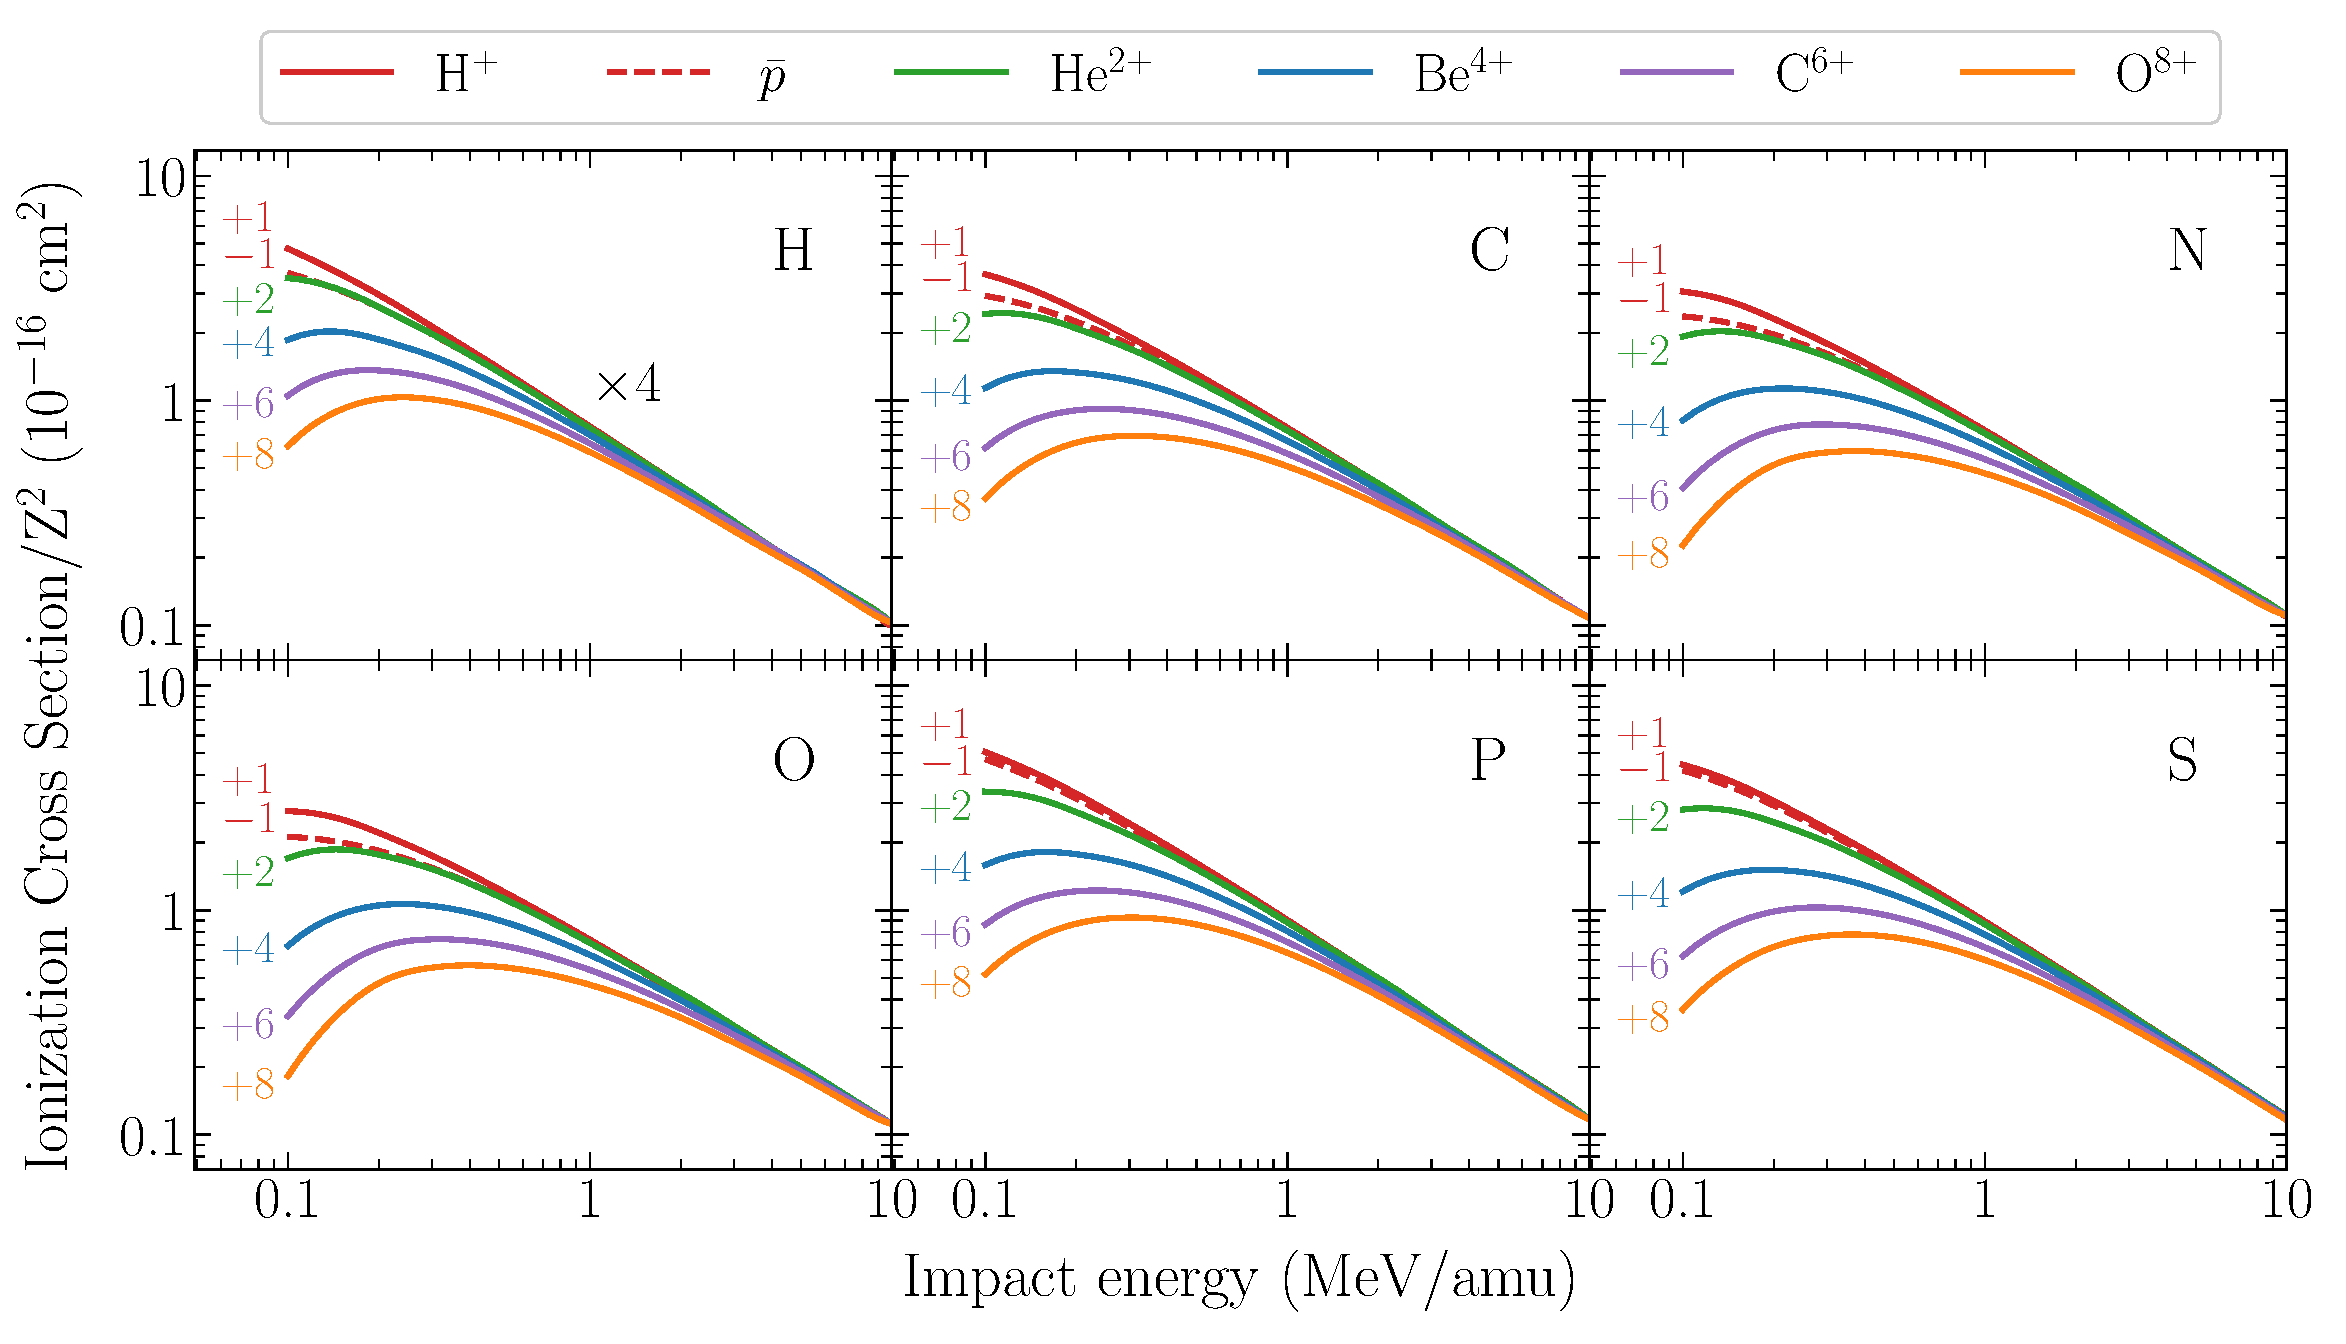
\includegraphics[width=0.9\textwidth]{ionmol/atomicscaling.eps}
\caption[Sección eficaz total de ionización atómica CDW reducida.]
{Sección eficaz total de ionización CDW reducida $\sigma_{\alpha}/Z^2$ 
de cuatro blancos atómicos relevantes. Curvas: cálculos teóricos CDW. 
Símbolos: ionización de H por impacto de H$^+$~\cite{Shah:81}; ionización 
por impacto de $e^-$ en H~\cite{Shah:87}, C~\cite{Brook:78}, 
N~\cite{Brook:78} y O~\cite{Thompson:95}.}
\label{fig:atomscaling}
\end{figure} 

La mayor parte de las moléculas orgánicas contienen átomos de hidrógeno, 
carbono, nitrógeno, oxígeno, fósforo y azufre. Los sistemas colisionales
que estudiamos a continuación están compuestos por cuatro blancos 
atómicos, $\alpha=$ H, C, N, O, y sies proyectiles incidentes: 
antiprotones $\bar{p}$, H$^{+}$, He$^{2+}$, Be$^{4+}$, C$^{6+}$, y 
O$^{8+}$. En la Fig.~\ref{fig:atomscaling} se muestran las secciones 
eficaces totales de ionización de los 24 sistemas blanco--proyectil 
resultantes usando el método CDW. Para comparar los resultados 
correspondiente a cada sistema colisional en una única figura, 
consideramos el hecho que en la primera aproximación de Born, la sección 
eficaz de ionización escala con el cuadrado de la carga del ion 
incidente, es decir $Z^{2}$. Las energías de impacto consideradas van de 
$0.1$ a 10 MeV/amu, donde el método CDW tiene validez. Particularmente, 
para los proyectiles de carga más altas, el valor de energía mínimo donde 
se espera que la CDW tenga validez aumenta hasta aproximadamente 400~keV. 
Nuestros resultados se comparan con secciones eficaces experimentales 
para el caso de ionización de H por impacto de H$^+$~\cite{Shah:81}. Se 
incluyen mediciones de ionización por impacto de electrones en 
H~\cite{Shah:87}, C~\cite{Brook:78}, N~\cite{Brook:78} y 
O~\cite{Thompson:95}, con la correspondiente conversión de equivelocidad, 
para energías incidentes superiores a 300~eV. Es esperable que en esta 
región de energía la ionización por impacto de H$^+$ y $e^-$ convergen. 
También realizamos cálculos similares con la FBA (no se muestran aquí), 
y corroboramos que ésta provee resultados confiables para valores de 
energía mayores a unos cuantos MeV/amu. Para nuestros resultados teóricos,
usamos el mismo color de línea para indicar la carga del proyectil en 
todas las figuras que se muestran a lo largo de este Capítulo: 
discontinua--roja, sólida--roja, azul, magenta, oliva y naranja para 
antiprotones, H$^{+}$, He$^{2+}$, Be$^{4+}$, C$^{6+}$, y O$^{8+}$, 
respectivamente. En el caso de los datos experimentales, se usan símbolos 
de los mismos colores para denotar la carga del ion incidente 
correspondiente. Los resultados de ionización de cada capa se pueden 
hallar en la Ref.~\cite{Miraglia:19}.

%%%%%%%%%%%%%%%%%%%%%%%%%%%%%%%%%%%%%%%%%%%%%%%%%%%%%%%%%%%%%%%%%%%%%%%%
\subsection{Distribución energética de electrones}
\label{subsec:meanener}
%%%%%%%%%%%%%%%%%%%%%%%%%%%%%%%%%%%%%%%%%%%%%%%%%%%%%%%%%%%%%%%%%%%%%%%%

En un medio biológico dado, la ionización directa debido al impacto de un 
ion representa solo una fracción del daño total. Los electrones 
secundarios, así como el retroceso de los iones del blanco, también 
contribuyen sustancialmente al daño total~\cite{Denifl:11}. Podemos 
considerar que la sección eficaz de ionización diferencial en función de 
la energía del electrón eyectado $E$ de la capa $nl$ del átomo $\alpha$,
$d\sigma_{\alpha nl}/dE$, es una función de distribución simple~\cite{Surdutovic:18}. Así, siguiente a Abril y 
coloboradores~\cite{Abril:15}, definimos un valor medio 
$\overline{E}_{\alpha}$, 
\begin{eqnarray}
\overline{E}_{\alpha} &=&\frac{\langle E_{\alpha}\rangle}{\langle
1\rangle}=\frac{1}{\sigma_{\alpha}}\sum\limits_{nl}\int dE\,E
\frac{d\sigma_{\alpha,nl}}{dE}\,,  
\label{eq:meanener} \\
\langle 1\rangle &=&\sigma_{\alpha}=\sum\limits_{nl}\int dE\,
\frac{d\sigma_{\alpha,nl}}{dE}\,. 
\label{eq:normener}
\end{eqnarray}
donde $\Sigma_{nl}$ tiene en cuenta la suma de las diferentes 
contribuciones de cada capa del elemento $\alpha$.

\begin{figure}
\centering
\includegraphics[width=0.9\textwidth]{ionmol/ener_mean.eps}
\caption[Distribución energética media de electrones emitidos.]
{Distribución energética media de electrones emitidos por la ionización 
debido al impacto de iones cargados dada por la Ec.~(\ref{eq:meanener}). 
Curvas: cálculos teóricos FBA con $Z=1$ (punteada) y CDW (sólidas y 
discontinua).}
\label{fig:emittedener}
\end{figure} 

Las energías medias de los electrones emitidos $\overline{E}_{\alpha}$ 
por H, C, N y O se muestran en la Fig.~\ref{fig:emittedener}. El rango 
de velocidad de impacto fue reducido a $v=10$~a.u. debido a las 
limitaciones numéricas en la expansión de esféricos armónicos dados por 
la Ec.~(\ref{eq:contwave}). A medida que la velocidad de impacto $v$ 
aumenta, también aumenta $\langle E_{\alpha}\rangle$ y $l_{\max}$, lo que 
resulta en la inclusión de funciones con muchas oscilaciones en el 
integrando. Más aún, el integrando de $\langle E_{\alpha}\rangle$ incluye 
la energía cinética $E$, que reduce su valor en la región de energías 
pequeñas y lo incrementa para valores grandes, haciendo que el resultado 
sea más sensible a los momentos angulares mayores. Independientemente, 
para $v>10$ a.u., la primera aproximación de Born es válida. 

En la Fig.~\ref{fig:emittedener} estimamos el valor de 
$\overline{E}_{\alpha}$ de los electrones emitidos en el rango de energía 
de 10 a 70 eV, para todos los blancos atómicos. Nuestros resultados 
concuerdan con los hallazgos experimentales~\cite{Surdutovic:18}. Como se 
puede observar en la figura, el valor de energía media es 
sorprendentemente sensible a la carga del proyectil $Z$, que puede 
duplicar los resultados de protón en la región intermedia, i.e., 
100--400 keV/amu. El efecto observado puede atribuirse al repulsión 
electrónica causada por los iones de carga múltiple en los electrones de 
baja energía. Este comportamiento no se puede encontrar en la primera 
aproximación de Born, donde la ley de escala $Z^2$ cancela la dependencia 
con $Z$ de la Ec.~(\ref{eq:meanener}). A altas energías, 
$\overline{E}_{\alpha}$ tiende a un valor universal para todos los iones, 
como puede verse en la Fig.~\ref{fig:emittedener}.

%%%%%%%%%%%%%%%%%%%%%%%%%%%%%%%%%%%%%%%%%%%%%%%%%%%%%%%%%%%%%%%%%%%%%%%%
\subsection{Distribución angular de electrones}
\label{subsec:meanang}
%%%%%%%%%%%%%%%%%%%%%%%%%%%%%%%%%%%%%%%%%%%%%%%%%%%%%%%%%%%%%%%%%%%%%%%%

\begin{figure}
\centering
\includegraphics[width=0.9\textwidth]{ionmol/ang_mean.eps}
\caption[Distribución angular media de electrones emitidos.]
{Distribución angular media de electrones emitidos por la ionización 
debido al impacto de iones cargados dada por Ec.~(\ref{eq:meanang}). 
Curvas: cálculos teóricos FBA con $Z=1$ (punteada) y CDW (sólidas y 
discontinua).}
\label{fig:emittedang}
\end{figure} 

Como mencionamos anteriormente, la emisión de electrones secundarios 
contribuye al daño total. Entonces, no sólo es esencial conocer la 
distribución de energía de los electrones eyectados, sino también la 
dirección a la que éstos son emitidos. Una vez más, podemos considerar 
que la sección eficaz diferencial de ionización es función del ángulo 
sólido de eyección del electrón $\Omega$, $d\sigma_{\alpha,nl}/d\Omega$, 
y puede expresarse como una función de distribución. Así, el ángulo medio 
de emisión $\overline{\theta}_{\alpha}$ se define como
\begin{eqnarray}
\overline{\theta}_{\alpha}&=&\frac{\langle\theta_{\alpha}\rangle}
{\langle 1\rangle}=\frac{1}{\sigma_{\alpha}}\sum\limits_{nl}
\int d\Omega\,\theta\,\frac{d\sigma_{\alpha,nl}}{d\Omega} 
\label{eq:meanang} \\
\langle 1\rangle &=&\sigma_{\alpha}=\sum\limits_{nl}\int d\Omega\,
\frac{d\sigma_{\alpha,nl}}{d\Omega}\,.
\end{eqnarray}

Los ángulos medios de emisión electrónica $\overline{\theta}_{\alpha}$ 
de los cuatro átomos y seis iones estudiados en esta sección se muestran 
en la Fig.~\ref{fig:emittedang}. Se puede observar una dependencia 
significativa de $\overline{\theta}_{\alpha}$ con $Z$ para todos los 
sistemas colisionales. Una vez más, este efecto no puede ser observado en 
la implementación del FBA (línea punteada).

En la emisión de electrones de baja energía, la dispersión angular es 
casi isotrópica~\cite{Rudd:92}. Un valor típico para el ángulo de 
eyección considerado en la literatura es 
$\overline{\theta}_{\alpha}\sim$~70\textdegree~\cite{Surdutovic:18}, el 
cual resulta bastante certero en el rango de validez de la FBA para 
cualquier blanco. Sin embargo, cuando se usa la aproximación de onda 
distorsionada, $\overline{\theta}_{\alpha}$ disminuye sustancialmente con 
$Z$ en la región de energía intermedia, como se observa en la 
Fig.~\ref{fig:emittedang}. Cuanto mayor sea la carga $Z$, menor será 
$\overline{\theta}$. Por supuesto, este efecto solo es válido en energías 
intermedias y no en el rango de altas energías.

Para ilustrar esta característica, consideramos el impacto de C$^{6+}$ 
con una energía de 500~keV sobre oxígeno. La primera aproximación de Born 
predice electrones emitidos con energías medias de $46.7$ eV y ángulos 
medios de 78\textdegree, mientras que la aproximación CDW establece 
energías medias de $62.5$~eV y un ángulo de emisión igual a 60\textdegree. 
Nuestros resultados sugieren una penetración más profunda de los 
electrones secundarios con una orientación más cercana a la dirección del 
ion. Podemos atribuir esta corrección de la dirección de avance al efecto 
de captura del continuo.

Además, la Fig.~\ref{fig:emittedang} proporciona una descripción 
ilustrativa del comportamiento de los antiprotones: el proyectil repele 
los electrones, siendo $\overline{\theta}_{\alpha}\sim$~90\textdegree. 
Nótese el descripción opuesta de protones y antiprotones dada por la CDW 
con respecto a la primera aproximación de Born; este fenómeno constituye 
un efecto Barkas angular.

%%%%%%%%%%%%%%%%%%%%%%%%%%%%%%%%%%%%%%%%%%%%%%%%%%%%%%%%%%%%%%%%%%%%%%%%
\section{El modelo estequiométrico}
\label{sec:SSM}
%%%%%%%%%%%%%%%%%%%%%%%%%%%%%%%%%%%%%%%%%%%%%%%%%%%%%%%%%%%%%%%%%%%%%%%%

El modelo estequiométrico simple (\acs{ssm}) que proponemos aquí para 
predecir secciones eficaces moleculares totales de ionización está basado 
en la aproximación de átomo independiente, también llamada regla aditiva 
de Bragg. Este modelo supone que los átomos que componen una molécula $M$ 
interactúan con el proyectil incidente pero no entre sí. Así, si 
suponemos que la molécula $M$ está compuesta por $n_{\alpha}$ átomos del 
elemento $\alpha$, el modelo estequiométrico aproxima la sección eficaz 
total de ionización de la molécula $\sigma_M$ como la suma de secciones 
eficaces totales de ionización de los átomos aislados $\sigma_{\alpha}$ 
ponderada por $n_{\alpha}$, 
\begin{equation}
\sigma_{M}=\sum\limits_{\alpha}n_{\alpha}\sigma_{\alpha}\,.  
\label{eq:sumion}
\end{equation}
Los blancos moleculares examinados a lo largo de este capítulo se 
clasifican en tres familias: CH, CHNO, y ADN, como se muestra en la 
Tabla~\ref{tab:families}.

\begin{table}
\begin{center}
\begin{tabular}{|p{0.08\textwidth}|p{0.8\textwidth}|}
\hline
\multirow{2}{*}{CH} & CH$_4$ (metano), C$_2$H$_2$ (acetileno), 
C$_2$H$_4$ (eteno), C$_2$H$_6$ (etano), \\ & C$_6$H$_6$ (benceno) \\
\hline
\multirow{2}{*}{CHNO} & C$_5$H$_5$N (piridina), C$_4$H$_4$N$_2$ (pirimidina), 
C$_2$H$_7$N (dimetilamina), \\ & CH$_5$N (monometilamina), 
C$_4$H$_8$O (THF) \\[0.2em]
\hline
\multirow{2}{*}{DNA} & C$_5$H$_5$N$_5$ (adenina), C$_4$H$_5$N$_3$O (citosina), 
C$_5$H$_5$N$_5$O (guanina), \\ & C$_5$H$_6$N$_2$O$_2$ (timina),
C$_4$H$_4$N$_2$O$_2$ (uracilo), H$_2$O (agua) \\
\hline
\end{tabular}
\caption[Blancos moleculares examinados y clasificados en tres familias.]
{Blancos moleculares de interés examinados en el presente trabajo y 
clasificados en tres familias.}
\label{tab:families}
\end{center}
\end{table}

En la Fig.~\ref{fig:crossDNA_1} reportamos las secciones eficaces de 
ionización totales reducidas con la carga del ión incidente, 
$\sigma_M/Z^2$, de las nucleobases del ADN --adenina, citosina, guanina y 
timina-- debido al impacto de iones de carga múltiple, que se obtienen a 
partir de la aproximación SSM y el método CDW. Para adenina, los datos 
experimentales disponibles para el impacto de protones~\cite{Iriki:11} 
tienen un excelente acuerdo con nuestras 
predicciones. La medición de C$^{4+}$~\cite{Sens:20} sobre adenina 
coincide con el modelo SSM--CDW dentro del margen de error. Si bien esta
data es preliminar, la comparación es alentadora en cuanto a la respuesta 
de nuestro modelo para la ionización de projectiles de carga múltiple. 
Por otro lado, los resultados teóricos de ionización de adenina debido a 
C$^{6+}$ discrepan con el valor experimental 
disponible~\cite{Bhattacharjee:19} en un factor dos. Esta discrepancia es 
intrigante ya que la medición se encuentra en el rango de altas energías, 
donde generalmente la teoría predice muy bien los experimentos.

No hemos encontrado en la bibliografía datos experimentales de ionización 
por impacto de iones cargados para el resto de las nucleobases de ADN.
Incluimos en la Fig.~\ref{fig:crossDNA_1} mediciones de ionización por 
impacto de electrones~\cite{Rahman:16}, con la correspondiente 
conversión de equivelocidad, para energías incidentes superiores a 
300~eV. En esta región, la sección eficaz de ionización por impacto de 
protones y electrones debería coincidir. Aunque las mediciones de impacto 
de electrones están por encima de nuestros hallazgos para todos los 
objetivos moleculares, vale la pena señalar que los resultados SSM--CDW
concuerdan muy bien con otras predicciones teóricas de ionización por 
impacto de electrones~\cite{mozejko2003,tan2018}.

\begin{figure}
\centering
\includegraphics[width=0.9\textwidth]{ionmol/adn1.eps}
\caption[Sección eficaz total de ionización reducida por $Z$ (Parte I).]
{Sección eficaz total de ionización CDW reducida $\sigma_{M}/Z^2$ como 
una función de la energía de impacto del ion. Símbolos: datos 
experimentales de impacto de protón~\cite{Iriki:11}, 
C$^{4+}$~\cite{Sens:20}, C$^{6+}$~\cite{Bhattacharjee:19}, y 
e$^-$~\cite{Rahman:16} con conversión de equivelocidad.}
\label{fig:crossDNA_1}
\end{figure} 

\begin{figure}
\centering
\includegraphics[width=0.9\textwidth]{ionmol/adn2.eps}
\caption[Sección eficaz total de ionización reducida por $Z$ (Parte II).]
{Sección eficaz total de ionización CDW reducida $\sigma_{M}/Z^2$ como 
una función de la energía de impacto del ion. Símbolos: datos 
experimentales de impacto de protón en uracilo~\cite{itoh2013}, 
pirimidina~\cite{wolff2014}, THF~\cite{wang2016} y agua~\cite{Luna2007,
Bolorizadeh86,H_Rudd85,toburen80}. Impacto de C$^{4+}$~\cite{Sens:20} y 
C$^{4+}$, C$^{6+}$, O$^{6+}$, F$^{6+}$, O$^{8+}$, y F$^{8+}$ en 
uracilo~\cite{agnihotri2012,agnihotri2013}. Ionización de agua por 
impacto de He$^{2+}$~\cite{Ohsawa05,He_Rudd85,toburen80}, 
C$^{6+}$~\cite{DalCappello2009,Bhattacharjee:17} y 
O$^{8+}$~\cite{Bhattacharjee:16}. 
Impacto de e$^-$~\cite{bug2017,wolf2019,fuss2009} con conversión de 
equivelocidad.}
\label{fig:crossDNA_2}
\end{figure} 

Las secciones eficaces de ionización total reducidas $\sigma_M/Z^2$ 
para uracilo, pirimidina, THF y agua se muestran en la 
Fig.~\ref{fig:crossDNA_2}. En uracilo, las mediciones experimentales de 
ionización por impacto de protones de Itoh~\textit{et al.}~\cite{itoh2013} 
tienen un buen acuerdo con nuestras predicciones. Sin embargo, para el 
mismo blanco, nuestra teoría predice secciones eficaces con un factor 
dos por encima de las mediciones experimentales de Agnihotri 
\textit{et al.}~\cite{agnihotri2012,agnihotri2013} para el impacto de 
iones de carga múltiple. No obstante, cabe señalar que nuestros 
resultados teóricos coinciden con los cálculos de Champion, Rivarola y 
colaboradores~\cite{agnihotri2012,champion2012}. Los cálculos recientes 
de Sarkadi~\cite{sarkadi2016} empleando el método CTMC también se 
encuentran por arriba de los valores experimentales de Tribedi y 
colaboradores~\cite{agnihotri2012,agnihotri2013}. Además, hemos incluimos 
una reciente medición experimental preliminar de Sens y 
colaboradores~\cite{Sens:20} para la ionización en uracilo debido al 
impacto de C$^{4+}$ que coincide con la teoría, lo que podría indicar 
algún problema con los valores experimentales de Agnihotri y 
colaboradores. 

Para pirimidina, mostramos una comparación de nuestros resultados con los 
datos experimentales de ionización por impacto de protones de Wolff
\textit{et al.}~\cite{wolff2014} y también para la ionización por impacto 
de electrones~\cite{bug2017} a altas energías. Las mediciones de impacto 
de electrones concuerdan con las predicciones SSM--CDW para energías 
superiores a 500~keV. Inesperadamente, las secciones eficaces de 
ionización por impacto de protones son significativamente más bajas que 
nuestros resultados. Una mayor cantidad de experimentos se encuentran 
disponibles para la ionización de la molécula de THF por impacto de 
H$^+$~\cite{wang2016} y de e$^-$~\cite{bug2017,wolf2019,fuss2009}. Los 
resultados que obtenemos de la combinación del SSM y las secciones 
eficaces atómicas CDW muestran un buen acuerdo general con esta data.

En el caso de la molécula de agua, los resultados experimentales son más 
abundantes que para el resto de los blancos. Los resultados 
experimentales~\cite{Luna2007,Bolorizadeh86,H_Rudd85,Ohsawa05,He_Rudd85,
toburen80,Bhattacharjee:16} coinciden con nuestras predicciones para 
todos los iones de carga múltiple examinados aquí, excepto para 
C$^{6+}$~\cite{DalCappello:09,Bhattacharjee:17}, donde la teoría 
sobrestima la ionización en un factor dos en el rango de altas energías. 
A diferencia de las nucleobases, pirimidina y THF, la estequiometría del 
agua es más simple; sin embargo, observamos que nuestro modelo responde 
bien incluso para predecir la ionización de moléculas pequeñas debido a 
la incidencia de iones pesados, tal como es el caso de O$^{6+}$.

%%%%%%%%%%%%%%%%%%%%%%%%%%%%%%%%%%%%%%%%%%%%%%%%%%%%%%%%%%%%%%%%%%%%%%%%
\section{Reglas de escala}
\label{sec:scaling}

%%%%%%%%%%%%%%%%%%%%%%%%%%%%%%%%%%%%%%%%%%%%%%%%%%%%%%%%%%%%%%%%%%%%%%%%
\subsection{Escala con electrones activos del blanco}
\label{subsec:ne_scaling}

%%%%%%%%%%%%%%%%%%%%%%%%%%%%%%%%%%%%%%%%%%%%%%%%%%%%%%%%%%%%%%%%%%%%%%%%
\subsubsection{Regla de Toburen}
\label{subsec:toburen}
%%%%%%%%%%%%%%%%%%%%%%%%%%%%%%%%%%%%%%%%%%%%%%%%%%%%%%%%%%%%%%%%%%%%%%%%

Toburen y colaboradores~\cite{Toburen:75,Toburen:76} propusieron el 
primer modelo fenomenológico completo y simple para la eyección de 
electrones de moléculas complejas. Los autores encontraron conveniente 
escalar la sección eficaz de ionización experimental en términos del 
número de electrones ligados débilmente, o activos, $n_e$. En general, 
este número está dado por la cantidad de electrones en la capa de 
valencia. Así, por ejemplo, para C, N y O, este número es igual al número 
total de electrones del átomo menos la capa K. 

Siguiendo a Toburen \textit{et al.}, definimos la sección eficaz de 
ionización escalada por el número de electrones débilmente ligado 
$\sigma_e$ para la molécula $M$ como
\begin{equation}
\sigma_e=\frac{\sigma_M}{n_e}\,, 
\label{eq:cross-ne} 
\end{equation}
donde $n_e=\sum_{\alpha}n_{\alpha}\nu_{\alpha}$ es el número total de 
electrones activos en el proceso colisional, y $\nu_{\alpha}$ es el 
número de electrones débilmente ligado en cada átomo $\alpha$. Para los 
blancos atómicos considerados aquí, los números de Toburen están dados 
por 
\begin{equation}
\nu_{\alpha}^T=\left\{ 
\begin{array}{ll}
1, & \text{para H,} \\
4, & \text{para C,} \\ 
5, & \text{para N,} \\ 
6, & \text{para O}\,.
\end{array}\right.
\label{eq:neToburen} 
\end{equation} 

La regla de Toburen se puede enunciar diciendo que $\sigma_{e}$ es un 
parámetro universal, que depende únicamente de la velocidad y naturaleza
del ion incidinte, aplicable en la región de $0.25$ a 5~MeV/amu. A 
muy altas energías, la probabilidad de ionizar electrones de la capa K 
es mayor. Así, en esta región, el número total de electrones activos 
será diferente. Una dependencia similar con el número de electrones 
ligados débilmente fue hallada por Itoh y coloboradores~\cite{itoh2013} 
para el impacto de protones sobre uracilo y adenina.

Siguiendo la ley de escala de Toburen, calculamos las secciones eficaces 
CDW escaladas con el número de electrones activos de Toburen, 
$\sigma_{e}^T$, para los blancos moleculares dados en la 
Tabla~\ref{tab:families}. Nuestros resultados se muestran en la 
Fig.~\ref{fig:newscaling}(a) en función de la energía de impacto para 
diferentes proyectiles de carga múltiple. Aunque la escala de Toburen se 
mantiene para altas energías, su desempeño no es muy satisfactorio: como 
se puede observar en la figura, la banda universal es bastante ancha.

\begin{figure}[t]
\centering
\includegraphics[width=0.9\textwidth]{ionmol/CDWscaling.eps}
\caption[Sección eficaz de ionización molecular escalada por $n_e$.]
{Sección eficaz de ionización molecular escalada por número de electrones 
débilmente ligados usando (a)~los números de Toburen $\nu_{\alpha}^T$, y 
(b) los números CDW $\nu_{\alpha}^{\text{CDW}}$ propuestos para las 
moléculas enlistadas en la tabla~\ref{tab:families}. Símbolos: 
datos experimentales de las Figs.~\ref{fig:crossDNA_1} y 
\ref{fig:crossDNA_2}.}
\label{fig:newscaling}
\end{figure}

%%%%%%%%%%%%%%%%%%%%%%%%%%%%%%%%%%%%%%%%%%%%%%%%%%%%%%%%%%%%%%%%%%%%%%%%
\subsubsection{Números CDW}
\label{subsec:CDW}
%%%%%%%%%%%%%%%%%%%%%%%%%%%%%%%%%%%%%%%%%%%%%%%%%%%%%%%%%%%%%%%%%%%%%%%%

La respuesta de nuestros resultados teóricos a la regla de escala de 
Toburen se puede entender inspeccionando la Fig.~\ref{fig:neCDW}. La 
figura muestra las secciones eficaces de ionización CDW de los átomos H, 
C, N y O debido al impacto de H$^+$ escaladas por el número de electrones 
activos de cada átomo. La Fig.~\ref{fig:neCDW}(a) muestra los resultados
CDW escalados con los números de Toburen dados por la 
Ec.~\ref{eq:neToburen}. La regla de Toburen no es satisfecha de manera 
apropiada por los cálculos CDW: para un valor de energía dado, los 
valores teóricos de ionización CDW escalados 
$\sigma_{\alpha}/\nu_{\alpha}^T$ de cada blanco atómico no son 
constantes. Por otro lado, si observamos los valores teóricos de 
ionización de O dados en la Fig.~\ref{fig:atomscaling}, notamos que éstos 
son muy similares a las secciones eficaces de C; esto pareciera sugerir 
que elnúmero de electrones activos en el átomo de O es cuatro en lugar de 
seis. De la misma manera, el número de electrones activos para N, que se 
obtienen a partir de los resultados teóricos CDW, también son diferentes 
de los dados por la Ec.~(\ref{eq:neToburen}). La Fig.~\ref{fig:neCDW}(b) 
muestra la respuesta de nuestros cálculos teóricos atómicos a estos 
nuevos valores.

\begin{figure}[t]
\centering
\includegraphics[width=0.9\textwidth]{ionmol/neCDW.eps}
\caption[Sección eficaz de ionización atómica escalada por $n_e$.]
{Sección eficaz de ionización atómica por impacto de H$^+$ escalada por 
electrón débilmente ligado usando (a)~los números de Toburen 
$\nu_{\alpha}^T$, y (b) los números CDW $\nu_{\alpha}^{\text{CDW}}$ }
\label{fig:neCDW}
\end{figure}

A partir del estudio sistemático de nuestros resultados teóricos de 
ionización en átomos, proponemos una optimización a la regla de Toburen. 
Así, el número total de electrones activos de la molécula $M$ en la 
Ec.~(\ref{eq:cross-ne}) está ahora dado por 
\begin{equation}
n_e'=\sum_{\alpha}n_{\alpha}\nu_{\alpha}^{\text{CDW}}\,,
\end{equation}
donde $\nu_{\alpha}^{\text{CDW}}$ son los números de electrones activos 
por átomo, que han sido optimizados a partir de las secciones eficaces 
de ionización CDW atómicas. Los números CDW están dados por
\begin{equation}
\nu_{\alpha }^{\text{CDW}} \sim\left\{ 
\begin{array}{ll}
1, & \text{para H,} \\
4, & \text{para C, N, y O}\,. \\ 
%4.5, & \text{para P y S}\,.
\end{array}
\right. 
\label{eq:neCDW}
\end{equation}

A partir de la Ec.~(\ref{eq:neCDW}), definimos nuevos números de 
electrones activos $n_e'$ para las moléculas consideradas hasta ahora.  
En la Tabla~\ref{tab:ne_molecules} mostramos algunos valores optimizados 
$n_e'$ y los números de Toburen $n_e$. Nuestros resultados son diferentes  
a los propuestos por Toburen, los cuales son utilizados por otros 
autores~\cite{itoh2013}, principalmente debido a las diferencias en los 
números de electrones activos del oxígeno. Las secciones eficaces 
moleculares escaladas por $n_e'$ se muestran en la 
Fig.~\ref{fig:newscaling}(b). Los datos experimentales para la ionización 
de adenina~\cite{Iriki:11,Sens:20,Bhattacharjee:19}, 
uracilo~\cite{itoh2013,Sens:20}, pirimidina~\cite{wolff2014}, 
THF~\cite{wang2016} y agua~\cite{Luna2007,Bolorizadeh86,H_Rudd85,
toburen80,Ohsawa05,He_Rudd85,DalCappello:09,Bhattacharjee:17,
Bhattacharjee:16} por impacto de iones cargados que se muestran en la 
Fig.~\ref{fig:newscaling}(b) validan nuestra optimización a la regla de 
escala de Toburen. También incluimos mediciones de ionización por 
impacto de electrones con conversión de equivelocidad en 
pirimidina~\cite{bug2017} y THF~\cite{bug2017,wolf2019,fuss2009}. Será 
interesante verificar nuestras predicciones con experimentos futuros, 
principalmente para estados de carga de proyectiles más altos.

\begin{table}
\begin{center}
\begin{tabular}{|p{0.12\textwidth}p{0.15\textwidth}p{0.03\textwidth}
p{0.03\textwidth}|p{0.12\textwidth}p{0.15\textwidth}p{0.03\textwidth}
p{0.03\textwidth}|}
\hline
Molécula        & Nombre      & $n_e$ & $n_e'$ & 
Molécula        & Nombre      & $n_e$ & $n_e'$ \\
\hline
H$_2$           & Dihidrógeno & 2      & 2     & 
C$_4$H$_4$N$_2$ & Pirimidina  & 30     & 28    \\
H$_2$O          & Agua        & 8      & 6     & 
C$_6$H$_6$      & Etano       & 30     & 30    \\
NH$_3$          & Amoníaco    & 8      & 7     & 
C$_4$H$_4$N$_2$O$_2$ & Uracilo & 40    & 36    \\
CH$_4$          & Metano      & 8      & 8     & 
C$_4$H$_5$N$_3$O & Citosina   & 42     & 37    \\
CH$_5$N         & Metilamina  & 14     & 13    & 
C$_5$H$_6$N$_2$O$_2$ & Timina & 48     & 42    \\
C$_2$H$_7$N     & Etilamina   & 20     & 19    & 
C$_5$H$_5$N$_5$ & Adenina     & 50     & 45    \\
C$_4$H$_8$O     & THF         & 30     & 28    & 
C$_5$H$_5$N$_5$O & Guanina    & 56     & 49    \\
\hline
\end{tabular}
\caption[Números de electrones activos moleculares de Toburen y CDW.]
{Número de electrones débilmente ligados según Toburen $n_e$ y 
optimización CDW~$n_e'$ para algunos blancos moleculares de interés 
biológico.}
\label{tab:ne_molecules}
\end{center}
\end{table}

\begin{figure}[t]
\centering
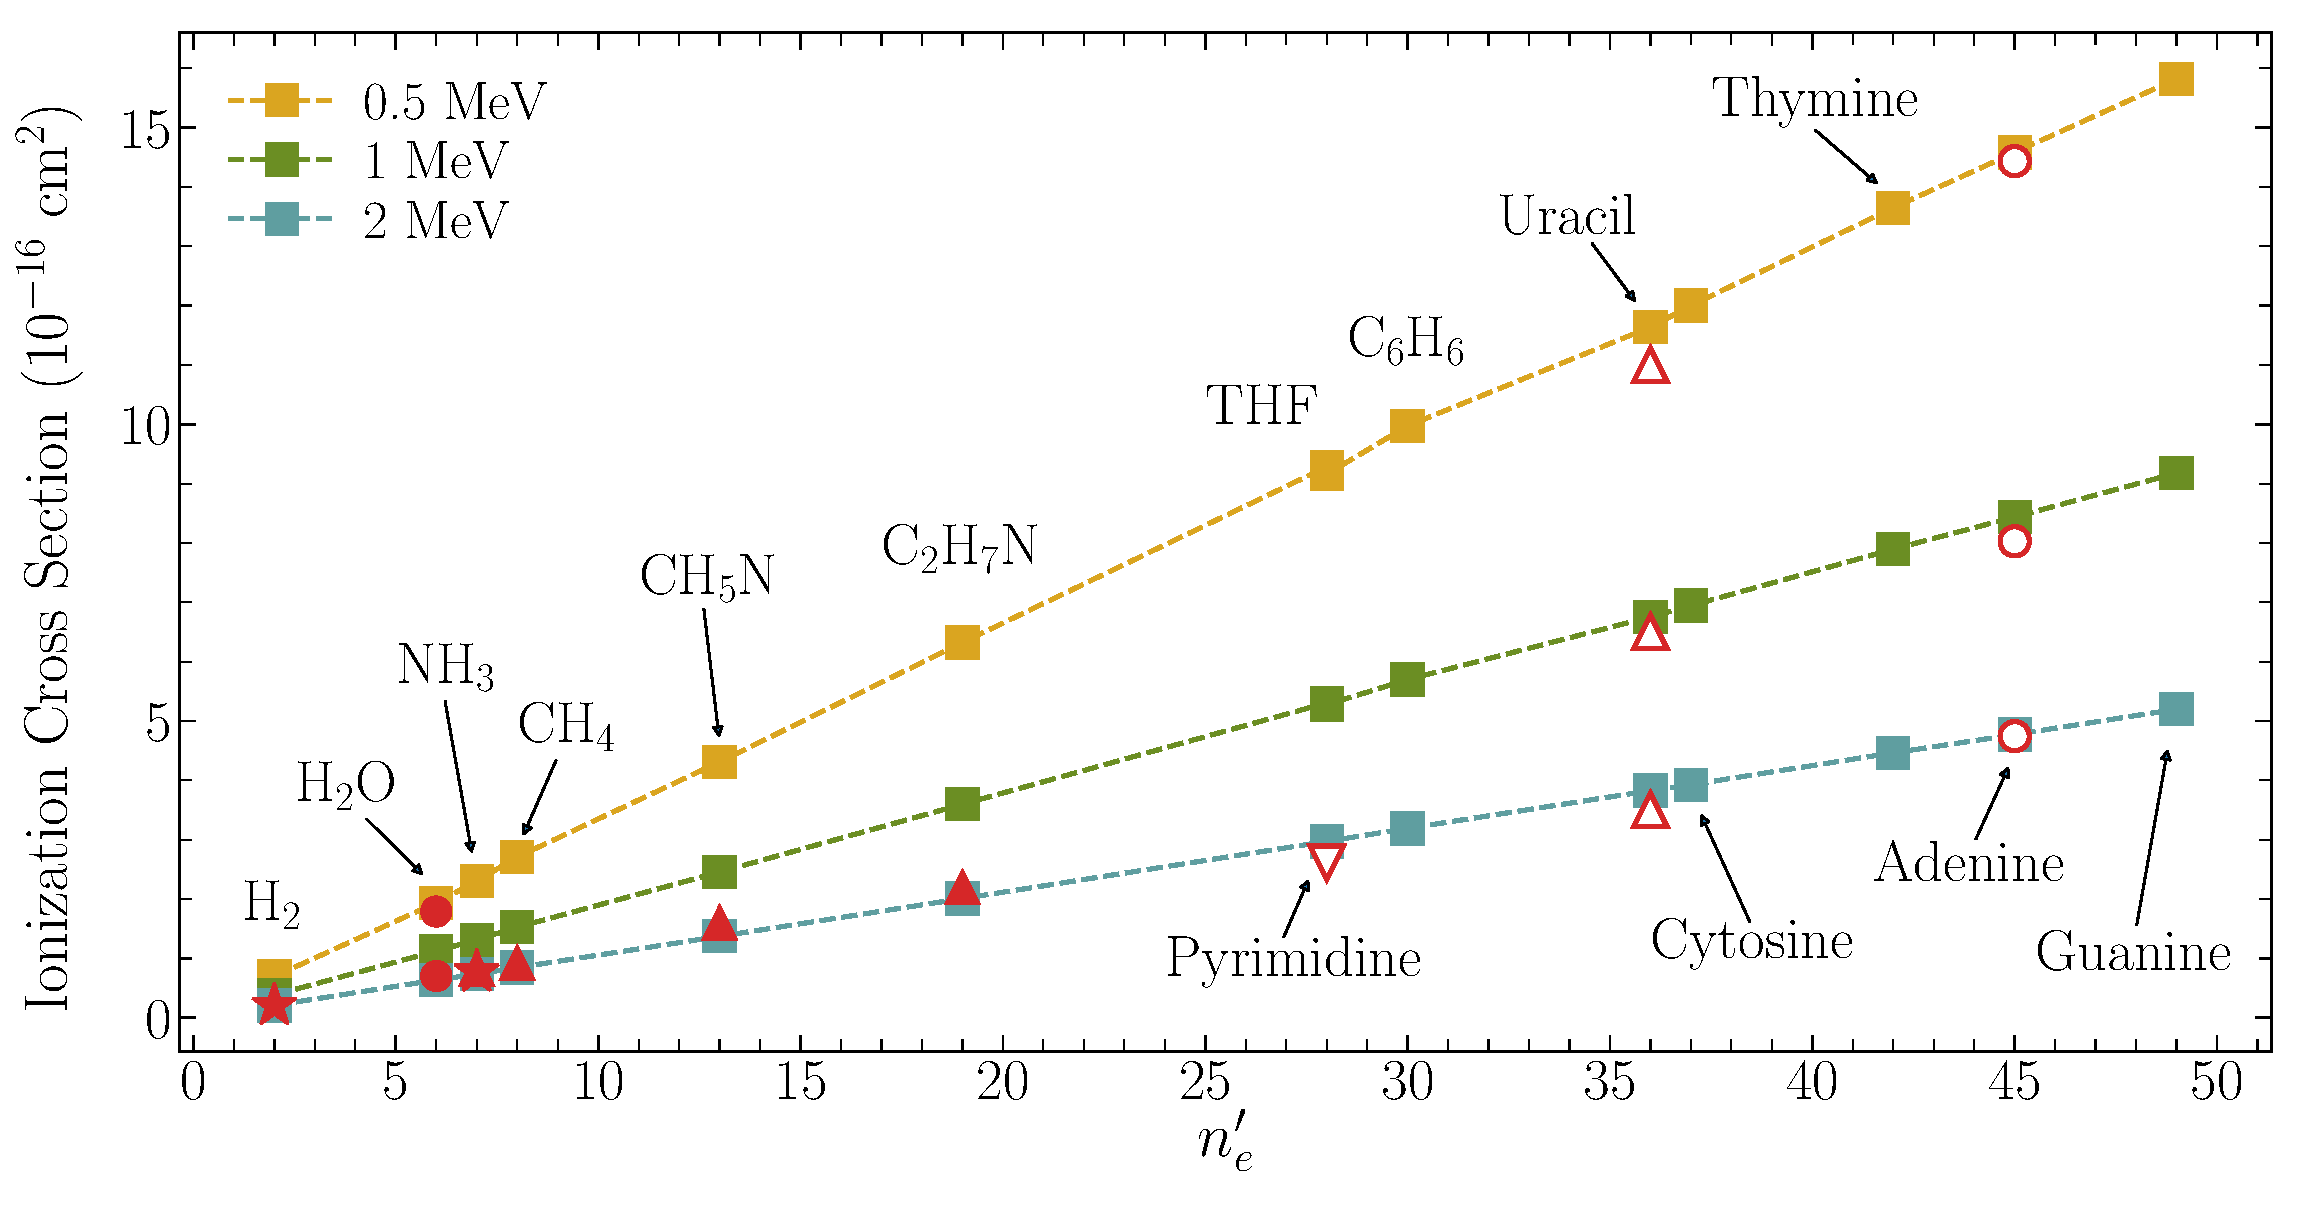
\includegraphics[width=0.9\textwidth]{ionmol/scale_ne.eps}
\caption[Ionización por impacto de protón en términos de $n_e'$.]
{Sección eficaz de ionización por impacto de protón a $0.5$, 1, y 2~MeV 
en términos del númbero de electrones activos dado por la 
Tabla~\ref{tab:ne_molecules}. Símbolos: 
\mbox{\Large$\circ$}~adenina~\cite{Iriki:11}, 
$\triangle$ uracilo~\cite{itoh2013}, 
$\bigtriangledown$ pirimidina~\cite{wolff2014}, 
$\blacktriangle$ C$_2$H$_7$N, CH$_5$N, metano y amoníaco~\cite{Lynch:76},
\mbox{\scriptsize$\bigstar$} amoníaco y H$_2$~\cite{Rudd:85}, y 
\mbox{\Large$\bullet$} agua~\cite{Luna2007}.}
\label{fig:recta}
\end{figure}

Podemos examinar de forma alternativa la escala definida por los números 
CDW dibujando las secciones eficaces de ionización de las moléculas en 
función de los valores dados para $n_e'$ según la 
Tabla~\ref{tab:ne_molecules} en ciertos valores de energía. Nuestros 
resultados se muestran en la Fig.~\ref{fig:recta} para energías de 
impacto de $0.5$, 1 y 2~MeV. Como puede observarse, las secciones 
eficaces de ionización CDW calculadas para todas las moléculas muestran 
una dependencia lineal con el número de electrones CDW $n_e'$ de la 
Tabla~\ref{tab:ne_molecules}. Obtenemos resultados similares, incluso 
para $E=10$~MeV. La comparación con los datos experimentales disponibles 
muestra una buena concordancia general, desde moléculas pequeñas, tales 
como H$_2$, CH$_4$ y NH$_3$, hasta las más complejas, como la adenina. 
Para los datos de ionización por impacto de electrón, los datos 
experimentales se interpolaron entre vecinos cercanos. 
%It is worth mentioning that an equivalent plot using the Toburen numbers 
%$n_e$ does not exhibit the straight lines obtained with the present scaling. 

%While finishing the present work, we became aware of an accepted 
%manuscript by L\"udde~\textit{et al.}~\cite{ludde2019} on total 
%ionization of biological molecules by proton impact, using the
%independent--atom--model pixel counting method~\cite{ludde2016,ludde2018}.
%The authors also raised a scaling  with $\nu_{\alpha}=4$ for C, N, and O. 
%The agreement with this independent method for proton impact reinforces 
%our multicharged--ion findings.

%%%%%%%%%%%%%%%%%%%%%%%%%%%%%%%%%%%%%%%%%%%%%%%%%%%%%%%%%%%%%%%%%%%%%%%%
\subsection{Escala con la carga del ion}
\label{sec:zscaling}
%%%%%%%%%%%%%%%%%%%%%%%%%%%%%%%%%%%%%%%%%%%%%%%%%%%%%%%%%%%%%%%%%%%%%%%%

A energías de impacto intermedias, la regla $Z^2$ no se cumple y se 
pueden considerar otras escalas en esta región. Encontramos en la 
literatura dos tipos de leyes de escala con la carga $Z$ del ion 
incidente aplicables en este rango de energías de impacto. La regla 
sugerida por Janev y Presnyakov~\cite{Janev:80} considera $\sigma/Z$ en 
función de $E/Z$ como la forma reducida \textit{natural} de la sección 
eficaz de ionización $\sigma$ y la energía de ion incidente $E$. Más 
recientemente, Montenegro y colaboradores~\cite{Dubois:13,Montenegro:13} 
sugirieron una expresión alternativa, la cual toma en cuenta que la 
sección eficaz es una función de $Z^2/E$ a altas energías. La escala 
propuesta, dada por
\begin{equation}
 \sigma/Z^{\alpha}=f(E/Z^{2-\alpha}),
\label{eq:Montenegro}
\end{equation}
mantiene la relación $Z^2/E$ para cualquier valor del parámetro $\alpha$. 
Los autores propusieron el valor $\alpha=4/3$ para la ionización de He y
H$_2$ debido al impacto de diversos iones cargados~\cite{Dubois:13}. 

Siguiendo el trabajo de Montenegro y colaboradores, optimizamos el 
parámetro~$\alpha$ de manera tal que los resultados obtenidos por la 
combinación del método CDW y SSM para los sistemas colisionales 
moleculares estudiados aquí convergan en el mayor rango de energías 
posible (de intermedias a altas). El resultado de dicha optimización es 
$\alpha=1.2$. La validez de este particular escaleo es evidente en la 
Fig.~\ref{fig:zreduced}, donde --para cada blanco-- las curvas SSM--CDW 
correspondientes a los diferentes iones se superponen. Es notable como 
los resultados teóricos son válidos para energías de impacto incluso por 
encima del máximo de las secciones eficaces, que corresponden a rangos de 
energías incidentes desde 50 keV para H$^+$ hasta 250 keV/amu para 
O$^{+8}$.

\begin{figure}
\centering
\includegraphics[width=0.9\textwidth]{ionmol/adn1_zscale.eps}
\caption[Sección eficaz de ionización reducida por $Z$ y $\alpha$ 
(Parte I).]
{Sección eficaz de ionización reducida $\sigma/Z^{\alpha}$ como función
de la energía incidente del ion $E/Z^{2-\alpha}$ con $\alpha=1.2$. 
Curvas: resultados teóricos CDW-SSM. 
Símbolos: datos experimentales de la Fig.~\ref{fig:crossDNA_1}.}
\label{fig:zreduced}
\end{figure} 

\begin{figure}
\centering
\includegraphics[width=0.9\textwidth]{ionmol/adn2_zscale.eps}
\caption[Sección eficaz de ionización reducida por $Z$ y $\alpha$ 
(Parte II).]
{Sección eficaz de ionización reducida $\sigma/Z^{\alpha}$ como función
de la energía incidente del ion $E/Z^{2-\alpha}$ con $\alpha=1.2$. 
Curvas: resultados teóricos CDW-SSM. 
Símbolos: datos experimentales de la Fig.~\ref{fig:crossDNA_2}.}
\label{fig:zreduced}
\end{figure} 

También examinamos los datos experimentales disponibles para los sistemas
ion-blanco bajo estudio~\cite{Iriki:11,Sens:20,Bhattacharjee:19,itoh2013,
wolff2014,wang2016,agnihotri2012,agnihotri2013,Luna2007,Bolorizadeh86,
H_Rudd85,He_Rudd85,toburen80,Ohsawa05,Bhattacharjee:17,DalCappello:09,
Bhattacharjee:16} con la regla de escala $Z^\alpha$. En el caso de los 
blancos con pocos o ningún dato experimental incluimos secciones eficaces 
experimentales de ionización por impacto de electrón~\cite{Rahman:16,
bug2017,wolf2019,fuss2009} a grandes velocidades con la conversión 
correspondiente. Como se observa, la mayor parte de los datos 
experimentales en la Fig.~\ref{fig:zreduced} confirma el escaleo sugerido 
aquí, incluso para O$^{+8}$ en agua~\cite{Bhattacharjee:16}. 

%%%%%%%%%%%%%%%%%%%%%%%%%%%%%%%%%%%%%%%%%%%%%%%%%%%%%%%%%%%%%%%%%%%%%%%%
\subsection{Escala con electrones activos y carga del ion}
\label{sec:nez_scaling}
%%%%%%%%%%%%%%%%%%%%%%%%%%%%%%%%%%%%%%%%%%%%%%%%%%%%%%%%%%%%%%%%%%%%%%%%

Considerando la reducción con la carga del ión incidente $Z^\alpha$ y el 
escaleo con el número de electrones activos del blanco, introducimos 
la sección eficaz de ionización molecular independiente $\tilde{\sigma}$, 
que se expresa como función de $\tilde{E}=E/Z^{2-\alpha}$, y está dada por
\begin{equation}
 \tilde{\sigma}\left(\tilde{E}\right)=\frac{\sigma_e}{Z^{\alpha}}
 =\frac{\sigma_M}{n_e'\,Z^{\alpha}}\,,
\label{eq:u-scaling}
\end{equation}
donde $\sigma_M$ es la sección eficaz de ionización de un blanco 
molecular, $n_e'$ es el número de electrones activos por molécula dado
en la Tabla~\ref{tab:ne_molecules}, y el parámetro es $\alpha=1.2$. La 
Fig.~\ref{fig:zalpha} muestra los valores teóricos y experimentales de 
$\tilde{\sigma}$ para todos los sistemas moleculares de la 
Tabla~\ref{tab:families}. Como se observa, la regla de escala combinada 
funciona muy bien y es independiente tanto de la naturaleza del ion 
incidente como de la complejidad del blanco molecular. Nuestros 
resultados teóricos SSM--CDW se ubican en una banda estrecha válida para 
cualquier ion incidente (reducida con $Z^\alpha$) en cualquier molécula
(escalada con el número de electrones activos $n_e'$) con una dispersión 
de aproximadamente $\pm 20\%$. Si consideramos los valores experimentales
disponibles, la incertidumbre de nuestra escala independiente crece a 
$\pm 30\%$, esquematizada en la Fig.~\ref{fig:zreduced} con un área gris. 
Notar que no hemos incluido en esta figura los resultados para uracilo de 
las Refs.~\cite{agnihotri2012,agnihotri2013}. 

\begin{figure}[t]
\centering
\includegraphics[width=0.9\textwidth]{ionmol/Zne_scaling.eps}
\caption[Sección eficaz de ionización reducida por $Z$ y $n_e$.]
{Sección eficaz de ionización reducida con la carga $Z$ del ion incidente
y escalada con el número de electrones activo $n_e$ del blanco molecular,
dado por la ecuación~(\ref{eq:u-scaling}) con $\alpha=1.2$. 
Curvas: resultados teóricos CDW-SSM. Símbolos: datos experimentales de 
las Figs.~\ref{fig:crossDNA_1} y \ref{fig:crossDNA_2}.}
\label{fig:zalpha}
\end{figure} 

Proponemos que la regla de escala independiente propuesta es válida para 
cualquier combinación ion--molécula. Para evaluar la generalidad de 
nuestro modelo, incluimos en la Fig.~\ref{fig:zreduced} un grupo de datos 
experimentales correspondientes a blancos moleculares no considerados en 
el diseño de esta regla, tales como las mediciones de 
Rudd~\textit{et al.}~\cite{Rudd:85,Rudd:83} para H$^{+}$ y He$^{+2}$ 
en N$_2$, O$_2$, CH$_4$, CO y CO$_2$, y los recientes experimentos de
Luna~\textit{et al.} \cite{Luna2019} de H$^{+}$ en CH$_4$. 

El buen acuerdo entre los resultados previstos por nuestro modelo y los
datos experimentales disponibles que se muestran en la 
Fig.~\ref{fig:zalpha} resume los principales resultados de esta 
investigación. Nuestro regla de escala independiente muestra ser eficaz 
no solo para predecir la ionización de los sistemas ion--blanco 
estudiados aquí sino también muestra potencial para reproducir una gran 
variedad de sistemas colisionales. Aunque los resultados teóricos 
SSM--CDW son válidos para energías por debajo del máximo de la sección 
eficaz de ionización, se puede observar en la Fig.~\ref{fig:zalpha} como 
el escaleo de los datos experimentales se extiene aún para valores de 
energía incidente menores. Esperamos que mediciones experimentales para 
otros iones y moléculas refuercen el modelo y escaleo propuesto.

%%%%%%%%%%%%%%%%%%%%%%%%%%%%%%%%%%%%%%%%%%%%%%%%%%%%%%%%%%%%%%%%%%%%%%%%
\section{Estructura molecular de los blancos}
\label{sec:molcalculations}
%%%%%%%%%%%%%%%%%%%%%%%%%%%%%%%%%%%%%%%%%%%%%%%%%%%%%%%%%%%%%%%%%%%%%%%%

Finalmente, para probar el rango de validez del SSM, realizamos un 
cálculo de estructura molecular de primeros principios para cinco 
nucleobases empleando el código {\sc gamess}. Los cálculos de energía de 
un centro se realizaron implementando el método restringido de 
Hartree--Fock con optimización de geometría y el conjunto de bases 
gaussianas 3-21G. 

\begin{figure}
\centering
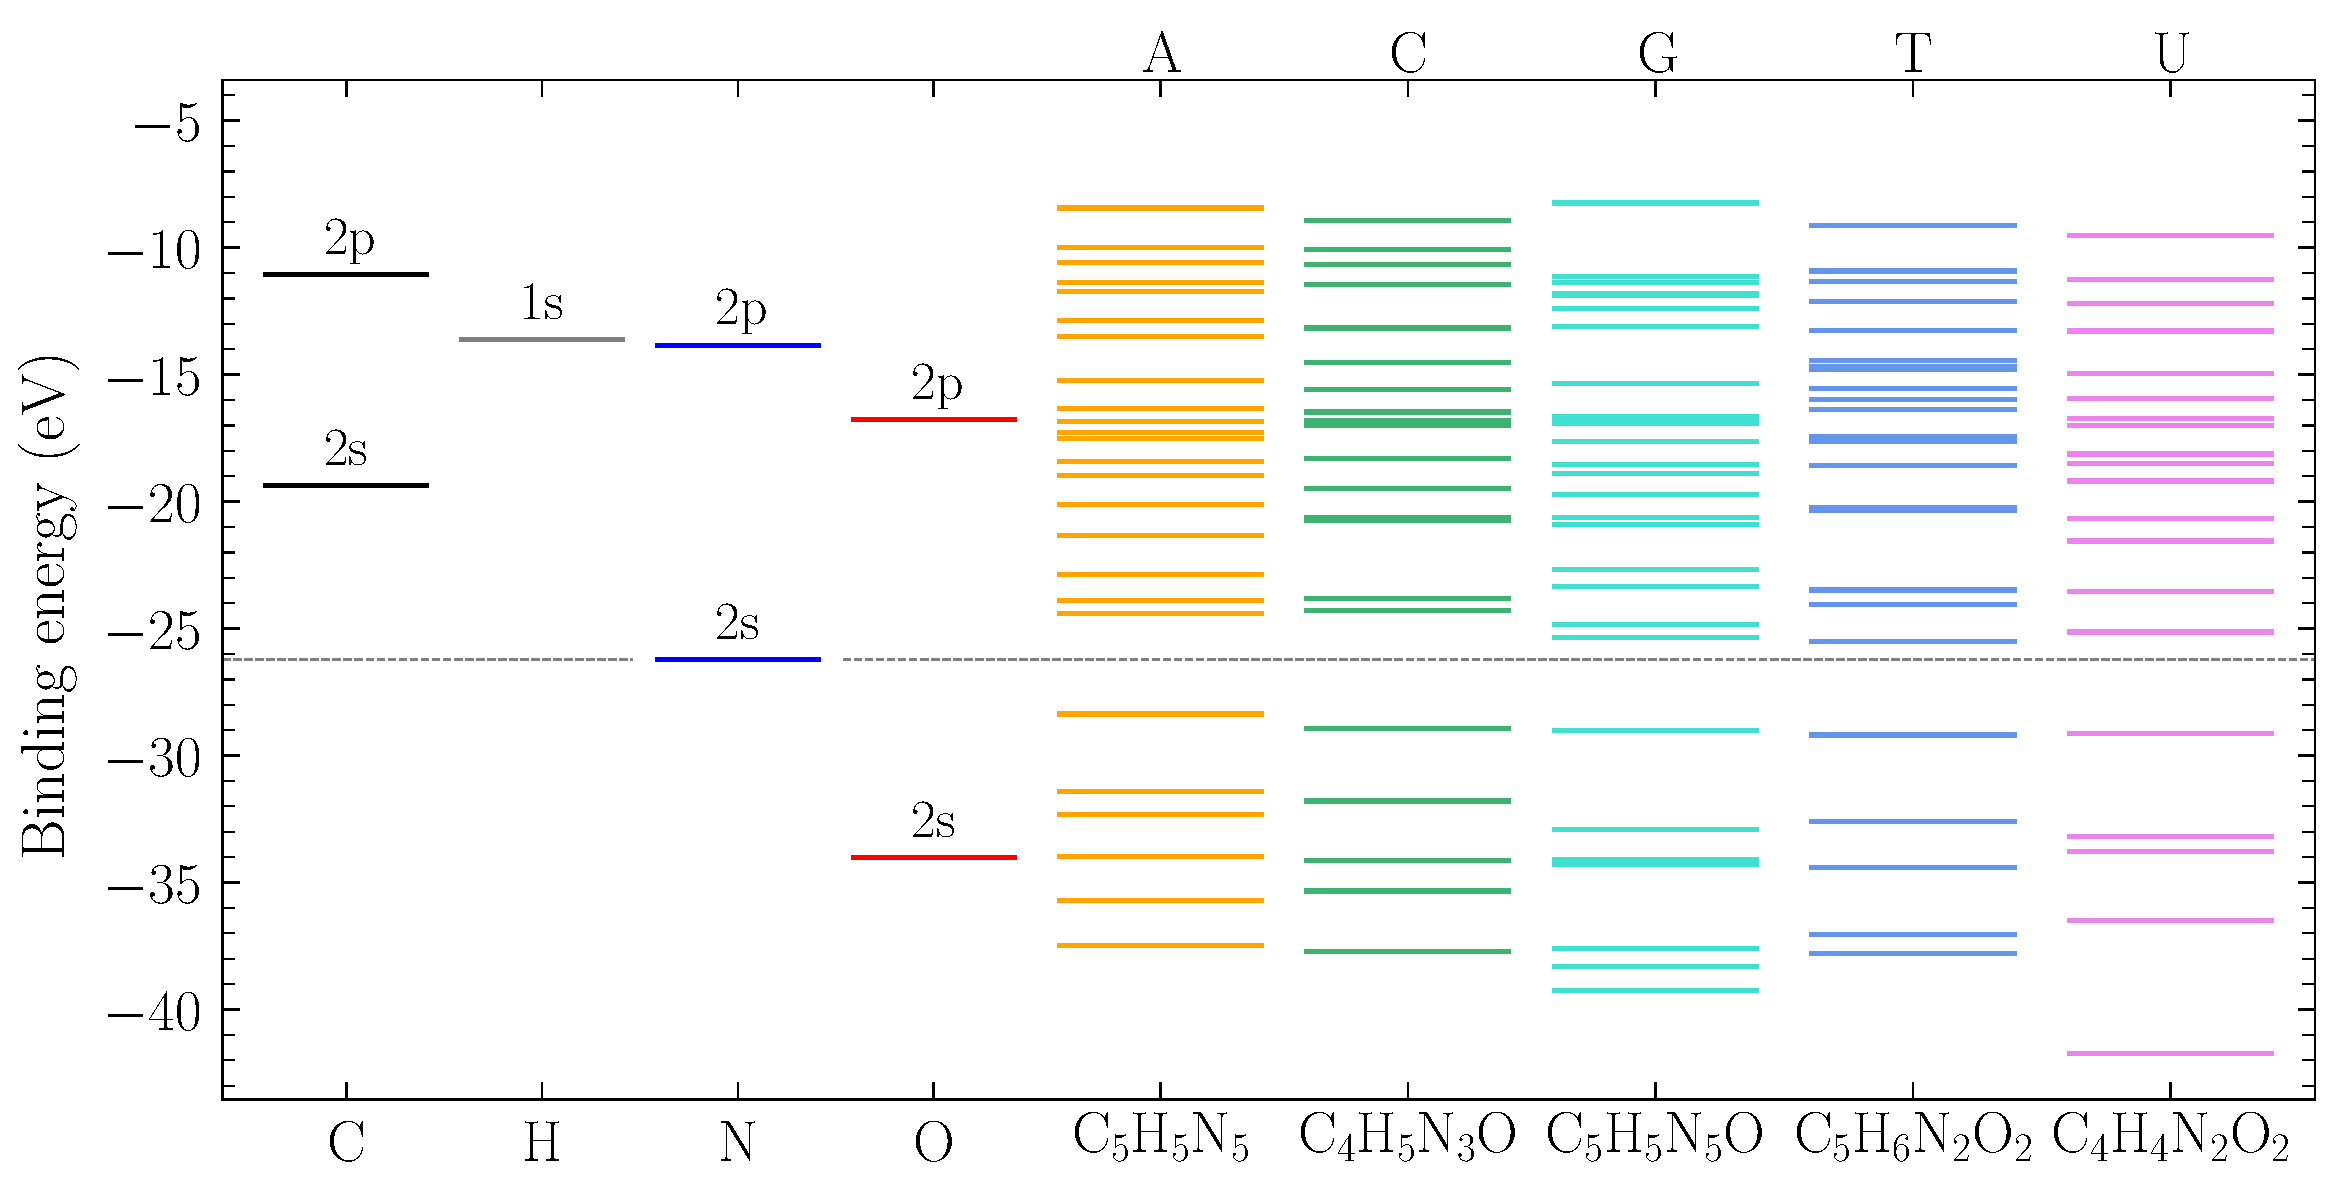
\includegraphics[width=0.9\textwidth]{ionmol/levelsDNA.eps}
\caption[Energías de ligadura moleculares teóricas de ADN y ARN.]
{Energías de ligadura moleculares teóricas de adenina, citosina, guanina, 
timina, y uracilo, comparado con los valores correspondientes de los 
átomos que las constituyen.}
\label{fig:bindener}
\end{figure}

En la Fig.~\ref{fig:bindener} se muestran las energías de ligadura 
molecular de los electrones de valencia para las nucleobases: adenina, 
citosina, guanina, timina y uracilo. Las energías de ligadura del orbital 
molecular más alto (HOMO) obtenidos concuerdan con los valores 
experimentales~\cite{Hush,Verkin,Dougherty} en un 2\% para todas las 
moléculas consideradas. En la izquierda de la Fig.~\ref{fig:bindener}, 
mostramos las energías atómicas de Hartree-Fock de los elementos 
constituyentes. Esta comparación nos da una idea de la distribución de 
los electrones débilmente ligados en las moléculas. Se traza una línea 
discontinua alrededor de $-26$~eV para separar la banda molecular en dos. 
Podemos considerar los niveles de energía atómica por encima de esta 
línea como los correspondientes a los electrones débilmente ligados de la 
Ec.~(\ref{eq:neCDW}). Por ejemplo, los electrones $2s$ y $2p$ del 
carbono se ubican por encima de la línea discontinua, que corresponde a 
los cuatro electrones dados por los números CDW. En el caso de O, solo 
los cuatro electrones de los orbitales 2p se encuentran por encima de la 
línea divisoria propuesta, que se corresponde con el número de electrones
débilmente ligados dado por el escaleo CDW. El caso del átomo de N no es 
tan directo; el número $\nu_{N}^{\text{CDW}}=4$ sugiere que sólo uno de 
los dos electrones de la capa $2s$ contribuye al esquema molecular.

%%%%%%%%%%%%%%%%%%%%%%%%%%%%%%%%%%%%%%%%%%%%%%%%%%%%%%%%%%%%%%%%%%%%%%%%
\subsection{Un modelo estequiométrico modificado}
%%%%%%%%%%%%%%%%%%%%%%%%%%%%%%%%%%%%%%%%%%%%%%%%%%%%%%%%%%%%%%%%%%%%%%%%

El modelo estequiométrico propuesto en la Sección~\ref{sec:SSM} considera 
a la molécula $M$ como un conjunto de átomos neutros aislados, lo cual es 
definitivamente irreal. Una primera mejora se puede sugerir asumiendo que 
los átomos no son efectivamente neutrales y que tienen una distribución 
dispar de los electrones dentro de la molécula. Esta característica puede 
expresarse mediante una carga efectiva $q_{\alpha}$ por átomo. La carga 
de Mulliken proporciona un valor posible para $q_{\alpha}$; sin embargo, 
existe una gran variedad de posibles distribuciones de 
carga~\cite{lee2003}.

\begin{table}
\begin{center}
\begin{tabular}{|p{0.12\textwidth}|p{0.08\textwidth}|p{0.08\textwidth}|p{
0.08\textwidth}|p{0.08\textwidth}|p{0.28\textwidth}|}
\hline
Molécula & C & H & N & O & Estequiometría de carga \\
\hline
Adenina & +0.32 & +0.23 & --0.55 &       & 
C$_{4.92}$H$_{4.77}$N$_{5.14}$ \\ 
\hline
Citosina & +0.28 & +0.21 & --0.56 & --0.53 & 
C$_{3.93}$H$_{4.79}$N$_{3.14}$O$_{1.13}$ \\ 
\hline
Guanina & +0.46 & +0.20 & --0.58 & --0.36 & 
C$_{4.89}$H$_{4.80}$N$_{5.15}$O$_{1.09}$ \\ 
\hline
Timina & +0.20 & +0.19 & --0.54 & --0.52 & 
C$_{4.95}$H$_{5.81}$N$_{2.13}$O$_{2.13}$ \\ 
\hline
Uracilo & +0.31 & +0.22 & --0.59 & --0.47 & 
C$_{3.92}$H$_{3.78}$N$_{2.15}$O$_{2.12}$ \\ 
\hline
\end{tabular}
\caption[Cargas efectivas medias de Mulliken por átomo]
{Cargas efectivas medias de Mulliken por átomo $q_{\alpha}$, y nueva formula
estequiométrica definida por la ecuación~(\ref{eq:newstoi}) para cinco
moléculas de ADN.}
\label{tab:newstoi}
\end{center}
\end{table}

Para tomar en cuenta este efecto, consideramos que el número total de 
electrones $Q_{\alpha }$ en el elemento $\alpha$ se distribuye de forma
dispar sobre todos los átomos $\alpha$. Por lo tanto, cada elemento  
$\alpha$ tendrá una carga $q_{\alpha}=Q_{\alpha}/n_{\alpha}$, que puede 
ser positiva o negativa. Este valor dependerá de la electronegatividad 
relativa respecto a los otros átomos~\cite{rappe1991}. Siguiendo esta 
idea, podemos estimar el número fraccional de átomos por molécula 
$n_{\alpha}'$, el cual está dado por 
\begin{equation}
n_{\alpha }^{\prime }=n_{\alpha }-
\frac{q_{\alpha }}{\nu_{\alpha }^{\text{CDW}}}
\label{eq:newstoi}
\end{equation}
En el caso de átomos neutrales, $q_{\alpha}=0$ y $n_{\alpha}'=n_{\alpha}$,
como dispone el SSM. En la Tabla~\ref{tab:newstoi}, mostramos un valor 
promedio de carga efectiva por átomo $q_{\alpha}$ de C, H, N, y O, para 
cinco moléculas del ADN, las cuales se obtuvieron a partir de los 
cálculos de estructura molecular descritos en la sección anterior.

Implementando la Ec.~(\ref{eq:newstoi}), es posible determinar una nueva 
fórmula estequiométrica de carga, la cual se da en la última columna de 
la Tabla~\ref{tab:newstoi}). Ahora, en vez de tener un número entero de 
átomos $n_{\alpha}$, tenemos un número fraccional dado por $n_{\alpha}'$. 
Se pueden calcular nuevas secciones eficaces moleculares, 
$\sigma'_{M}=\sum_{\alpha}n_{\alpha}'\sigma_{\alpha}$ considerando tales 
valores. Se calcularon errores relativos de las secciones eficaces de 
ionización para las bases de ADN de la Tabla~\ref{tab:newstoi}. Las 
diferencias obtenidas fueron menores de 3\%, lo cual indica que el modelo 
estequiométrico es un modelo robusto con el que se pueden modelar este 
tipo de moléculas complejas dentro del margen de error esperado.

%%%%%%%%%%%%%%%%%%%%%%%%%%%%%%%%%%%%%%%%%%%%%%%%%%%%%%%%%%%%%%%%%%%%%%%%
\section{Conclusiones}
%%%%%%%%%%%%%%%%%%%%%%%%%%%%%%%%%%%%%%%%%%%%%%%%%%%%%%%%%%%%%%%%%%%%%%%%

En este capítulo, hemos estudiado la ionización de blancos moleculares 
de interés biológico debido al impacto de iones de carga múltple. Se han
calculado secciones eficaces de ionización de gran número de blancos 
moleculares de interés biologico conteniendo H, C, N y O por el impacto 
de antiprotones, H$^{+}$, He$^{2+}$, Be$^{4+}$, C$^{6+}$, y O$^{8+}$. 
Nuestras prediciones teóricas han sido obtenidas combinando la 
implementación del método de onda continua distorsionada con estado 
inicial de Eikonal para blancos atómicos (descritos con potenciales 
efectivos DIM), para modelar el proceso colisional, y el modelo 
estequiométrico simple, para aproximar la estructura de las moléculas. 
Presentamos secciones eficaces de ionización total para adenina, 
citosina, timina, guanina, uracilo, THF y agua, siendo comparadas a su 
vez con datos experimentales disponibles. 

Estudiamos y calcularon valores medios de energía y ángulo de emisión de 
los electrones ionizados de blancos atómicos, que son de importancia en 
el daño secundario de las colisiones con iones. Nuestros resultados 
muestran una clara dependencia de estos valores con la carga del ion $Z$. 
Para un blanco dado, a medida que $Z$ aumenta, $\overline{E}_{\alpha}$ 
también aumentan. Por otro lado, $\overline{\theta}_{\alpha}$ decrece, lo 
que muestra una clara tendencia a la dirección del ion. A energía de 
impacto mayores a 2~MeV/amu, estos valores convergen a la primera 
aproximación de Born, la cual establece la simple ley de escala $Z^{2}$. 

Propusimos tres reglas de escala para las secciones eficaces de 
ionización para blancos de interés biológico por cuatro iones desnudos. 
Primero, exploramos la ampliamente usada regla de escala de Toburen, que 
escala la sección eficaz de ionización molecular con un determinado 
número de electrones débilmente ligados. Luego, a partir de los 
resultados CDW para los atómos H, C, N y O, encontramos que la respuesta 
de las secciones eficaces de ionización puede ser optimizada 
normalizándolas con diferentes números de electrones activos en la 
colisión. Así, definimos la primera regla de escala con el número de 
electrones activos CDW, la cual provee buenos resultados para los 
sistemas proyectil--molécula estudiados aquí. La comparación con los 
datos experimentales refuerza nuestros hallazgos. Además, probamos la 
regla de escala CDW mediante la inclusión de datos experimentales de 
ionización de H$_2$, metano y amoníaco por impacto de protones, los 
cuales muestran una buena concordancia en el rango de energías 
intermedias a altas. La segunda regla de escala propuesta considera el 
ion incidente, reduciendo la naturaleza del proyectil mediante el escaleo 
de la sección eficaz de ionización con la carga del ión, $Z^{\alpha}$, 
como una función de la energía incidente reducida $E/Z^{2-\alpha}$, 
siendo $\alpha=1.2$. La última regla que proponemos combina el escaleo de 
la sección eficaz de ionización total con el número de electrones activos 
CDW y la reducción con la carga del ión, $Z^{\alpha}$, lo cual conduce a 
una ley de escala independiente de la carga del ion y el blanco 
molecular. Las tres reglas de escala obtenidas mediante nuestro modelo 
SSM--CDW para los 80 sistemas colisionales examinados fueron comparadas 
con datos experimentales disponibles. Luego, la generalidad de nuestra 
regla de escala independiente fue inspeccionada mediante la inspección
de un número significativo de datos experimentales para otros sistemas 
colisionales (no considerados previamente), probando ésta ser válida 
incluso para energías fuera del rango de validez del método SSM--CDW.

Finalmente, realizamos cálculos de estructura molecular para las 
nucleobases del ADN. Al inspeccionar las energías de ligadura moleculares 
obtenidas mediante cálculos mecanicocuánticos de primeros principios, 
pudimos comprender el número de electrones resultantes de la optimización 
basada en los cálculos CDW. Intentamos mejorar el modelo estequiométrico 
utilizando la carga de Mulliken para obtener proporciones fraccionarias 
en lugar de enteras para el número de átomos constituyentes. No 
encontramos una corrección sustancial, lo que indica que el SSM funciona 
bastante bien. Los presentes resultados refuerzan la exactitud del modelo 
estequiométrico simple y la aproximación CDW para tratar la ionización de 
moléculas complejas por el impacto de iones cargados en el rango de 
energía intermedia a alta. 


\chapter{Conclusiones generales}
\label{chap:conclusiones}





\chapter*{Publicaciones asociadas}%
\addcontentsline{toc}{chapter}{Publicaciones asociadas}%

\begin{enumerate}

\item
A.M.P. Mendez, D.M. Mitnik, J.E. Miraglia,
\textit{Depurated Inversion Method for Orbital-Specific Exchange Potentials},
Int. J. Quantum Chem. \textbf{116}, 1882 (2016). \\
DOI:~\href{http://www.doi.org/10.1002/qua.25295}{10.1002/qua.25295}

\item
A.M.P. Mendez, D.M. Mitnik, J.E. Miraglia, 
\textit{Local Effective Hartree-Fock Potentials Obtained by the Depurated Inversion Method},
Adv. Quant. Chem. \textbf{76}, 117--132 (2018). \\
DOI:~\href{http://www.doi.org/10.1016/bs.aiq.2017.07.004}{10.1016/bs.aiq.2017.07.004}

\item
A.M.P. Mendez, D.M. Mitnik, J.E. Miraglia, 
\textit{Collision processes using effective potentials},
Adv. Quant. Chem. \textbf{79}, 179--200 (2019). \\
DOI:~\href{http://www.doi.org/10.1016/bs.aiq.2019.05.003}{10.1016/bs.aiq.2019.05.003}

\item
D.M. Mitnik, A.M.P. Mendez, J.E. Miraglia, 
\textit{Reply to ``Comment on `Depurated Inversion Method for Orbital-Specific
Exchange Potentials' ''}, 
Int. J. Quantum Chem. \textbf{120}, e26102 (2020). \\
DOI:~\href{http://www.doi.org/10.1002/qua.26102}{10.1002/qua.26102}

\item
A.M.P. Mendez, C.C. Montanari, D.M. Mitnik, 
\textit{Relativistic atomic structure calculations of heavy targets for inelastic collisions},
Nucl. Instrum. Methods Phys. Res. B, \textbf{460}, 114-118 (2019). \\
DOI:~\href{http://www.doi.org/10.1016/j.nimb.2019.02.002}{10.1016/j.nimb.2019.02.002}

\newpage
\item
C.C. Montanari, P. A. Miranda, E. Alves, A. M. P. Mendez \textit{et al.},
\textit{Stopping power of hydrogen in hafnium and the importance of relativistic 4f electrons},
Phys. Rev. A \textbf{101}, 062701 (2020). \\
DOI:~\href{http://www.doi.org/10.1103/PhysRevA.101.062701}{10.1103/PhysRevA.101.062701} 

\item
A.M.P. Mendez, C.C. Montanari, J.E. Miraglia,
\textit{Ionization of biological molecules by multicharged ions using the stoichiometric model},
J. Phys. B, \textbf{53}, 055201 (2020). \\
DOI:~\href{http://www.doi.org/10.1088/1361-6455/ab6052}{10.1088/1361-6455/ab6052}

\item
A.M.P. Mendez, C.C. Montanari, J.E. Miraglia,
\textit{Scaling rules for the ionization of biological molecules by highly charged ions},
J. Phys. B, \textbf{53}, 175202 (2020). \\
DOI:~\href{http://www.doi.org/10.1088/1361-6455/ab9c36}{10.1088/1361-6455/ab9c36}

\item
A.M.P. Mendez, J.I. Di Filippo, S.D. López, D.M. Mitnik,
\textit{Bayesian atomic structure calculations for collisional problems},
J. Phys.: Conf. Ser. \textbf{1412}, 132027 (2020). \\
DOI:~\href{http://www.doi.org/10.1088/1742-6596/1412/13/132027}{10.1088/1742-6596/1412/13/132027}

\end{enumerate}


\appendix

%%%%%%%%%%%%%%%%%%%%%%%%%%%%%%%%%%%%%%%%%%%%%%%%%%%%%%%%%%%%%%%%%%%%%%%%
\chapter{Ecuación normal}
%%%%%%%%%%%%%%%%%%%%%%%%%%%%%%%%%%%%%%%%%%%%%%%%%%%%%%%%%%%%%%%%%%%%%%%%
\label{app:ecnormal}

Las semillas iniciales dadas por la ecuación normal se obtienen al 
minimizar la función
\begin{equation}
 \beta(x_i) = y(x_i) - f(x_i,\lambda_1,\lambda_2,\dots,\lambda_m)\,,
\end{equation}
que es la diferencia entre la curva a ser ajustada, $y(r)$, y la función
analítica implementada para tal fin, $f(r)$. En el esquema de la 
inversión depurada, $y(r) = Z_{nl}^{\mathrm{HF}}(r)$ corresponde a la 
carga invertida, y $f(r) = Z_{nl}^{\mathrm{DIM}}(r)$ corresponde a la 
forma analítica que se ha fijado para la carga (la 
Ec.~(\ref{eq:atomzDIM}) para átomos y la Ec.~(\ref{eq:molzDIM}) para 
moléculas). Con el fin de minimizar $\beta(x_i)$ respecto a los $m$ 
parámetros $\lambda_j$ que determinan $f$, definimos los elementos de 
matriz $A_{ij}$,
\begin{equation}
  A_{ij} \equiv \frac{d\beta(x_i)}{d\lambda_j} =
 \frac{df(x_i,\lambda_1,\lambda_2,\dots, \lambda_m)}{d\lambda_j}
\end{equation}
Así, obtenemos el sistema de ecuaciones $[A] \,[d\lambda] = [d\beta]$, 
donde
\begin{equation}
 \left[
 \begin{array}{c}
  d\beta(x_1) \\
  d\beta(x_2) \\
  \vdots \\
  d\beta(x_n) \\
 \end{array}
 \right] =
 \left[
 \begin{array}{cccc}
  A_{11} & A_{12} & \cdots & A_{1m} \\
  A_{21} & A_{22} & \cdots & A_{2m} \\
  \vdots & \vdots & \ddots & \vdots \\
  A_{n1} & A_{n2} & \cdots & A_{nm} \\
 \end{array}
 \right]
 \left[
 \begin{array}{c}
 d\lambda_1 \\
 d\lambda_2 \\
 \vdots \\
 d\lambda_m \\
 \end{array}
 \right] \,.
\end{equation}
Multiplicando ambos lados de la ecuación por la matriz traspuesta 
$[A]^{T}$,
\begin{equation}
  \left[ A \right]^T \left[ A \right]\left[ d\lambda \right] =
  \left[ A \right]^T \left[ d\beta \right]\,,
\end{equation}
se obtiene un sistema de ecuaciones que se resuelve con rutinas 
numéricas estándar. Así, la solución $[d\lambda]$ permite obtener los 
parámetros iniciales que minimizan $[\beta]$.

%%%%%%%%%%%%%%%%%%%%%%%%%%%%%%%%%%%%%%%%%%%%%%%%%%%%%%%%%%%%%%%%%%%%%%%%
\chapter{Método de $R$-Matrix}
%%%%%%%%%%%%%%%%%%%%%%%%%%%%%%%%%%%%%%%%%%%%%%%%%%%%%%%%%%%%%%%%%%%%%%%%
\label{app:rmatrix}

% Griffin & Pindzola 2007

En la región interna, la función de onda total $\Psi_E$ del sistema 
electrónico $(N+1)$ para cualquier valor de energía $E$ se expande en 
términos de las funciones de base de $R$-Matrix $\Psi_k$ como
\begin{equation}
\Psi_E=\sum_k A_{Ek}\Psi_k\,.
\label{eq:RM-wavefn}
\end{equation}
La funciones de base $\Psi_k$ están dadas por
\begin{equation}
\Psi_k=\mathcal{A}\sum_{ij}a_{ijk}\bar{\Phi}_i u_{j}
+\sum_j b_{jk}\phi_j\,,
\label{eq:RM-basisfn}
\end{equation}
donde las funciones $u_{ij}$ constituyen un conjunto finito de orbitales 
de base, que se usan para representar las funciones de onda del continuo,
$\bar{\Phi}_i$ se forman acoplando las funciones $\Phi_i$ dadas por la 
Ec.~(\ref{eq:phi-RM}), $\phi_j$ son los orbitales del sistema $(N+1)$ 
que se construyen adicionando un electrón a los orbitales del blanco, y 
el operador $\mathcal{A}$ 
antisimetriza la coordenada del electrón dispersado con la coordenada 
del electrón del blanco $N$-ésimo. Los coeficientes $a_{ijk}$ y $b_{jk}$ 
se determinan diagonalizando el Hamiltoniano $H^{N+1}$ del sistema de 
electrones $(N+1)$ en la región interna,
\begin{equation}
\langle\Psi_k\left|H^{N+1}\right|\Psi_k'\rangle=E_k^{N+1}\delta_{kk'}\,.
\label{eq:RM-N+1Hamilt}
\end{equation}

El radio de la región interna $a$ se elije de manera tal que los 
orbitales radiales $P_{nl}$ del sistema de $N$ electrones del blanco 
están contenidos totalmente; esto es, \mbox{$P_{nl}\approx 0$ para 
$r>a$.} Para 
cada valor de momento angular $l$, los orbitales de la base del continuo 
$u_{ij}$ se determinan de la ecuación
\begin{equation}
\left[-\frac{1}{2}\frac{d^2}{dr^2}+\frac{l(l+1)}{2r^2}+V(r)
-\frac{k_j^2}{2}\right]u_{ij}(r)=-\sum_i\lambda_{ji}P_{n_il}(r)\,,
\label{eq:RM-difeq-uj}
\end{equation}
imponiendo las condiciones de borde 
\begin{equation}
u_{ij}(0)=0\,,\qquad\frac{a}{u_{ij}(a)}\frac{du_{ij}}{dr}\bigg|_{r=a}=b\,,
\end{equation}
y la condición de ortonormalidad.
El potencial $V(r)$ se define de forma conveniente para representar la
distribución de carga del blanco atómico y los multiplicadores de 
Lagrange $\lambda_{ji}$ se utilizan para forzar la ortonormalidad de las
bases del continuo con todos los orbitales ligados $P_{n_il}(r)$ con el
mismo momento angular $l$. En general, el valor de la segunda condición 
de borde $b$ es arbitraria y usualmente se asume igual a cero.

Definiendo la variable
\begin{equation}
w_{ik}=\sum_j a_{ijk}u_{ij}\,,
\end{equation}
la función de onda radial del electrón dispersado en el canal $i$ con 
energía $E$ resulta
\begin{equation}
y_i=\sum_kA_{Ek}w_{ik}\,.
\end{equation}
Se puede demostrar~\cite{Burke:75}, que los coeficientes $A_{Ek}$ 
están dados por
\begin{equation}
A_{Ek}=\frac{1}{2a\left(E_k^{N+1}-E\right)}\sum_jw_{jk}(a)
\left(a\frac{dy_j}{dr}-by_j\right)\bigg|_{r=a}\,.
\end{equation}
Así, la función de onda radial dispersada en el límite entre las 
regiones interna y externa se define como
\begin{equation}
y_i(a)=\sum_j R_{ij}\left(a\frac{dy_j}{dr}-by_j\right)\bigg|_{r=a}\,,
\end{equation}
donde $R_{ij}$ es un elemento de la matriz $R$ dado por
\begin{equation}
R_{ij} = \frac{1}{2a}\sum_k\frac{w_{ik}(a)w_{jk}(a)}{E_k^{N+1}-E}\,.
\label{eq:RM-elements}
\end{equation}
Las amplitudes de superficie $w_{ik}(a)$ y los polos $E_k^{N+1}$ de la 
matriz $R$ se determinan mediante los autovalores y autovectores del 
Hamiltoniano del sistema de $(N+1)$ electrones dado por la 
Ec.~(\ref{eq:RM-N+1Hamilt}). Los términos en la sumatoria que define 
$R_{ij}$ representan tanto los procesos colisionales resonantes y no 
resonantes, así como los efectos de interferencia entre ambos.

La mayor fuente de error en este método surge por el número finito de 
términos en la expansión de $R$-Matrix de la Ec.~(\ref{eq:RM-wavefn}), y 
por lo tanto, en el truncamiento en la sumatoria en la 
Ec.~(\ref{eq:RM-elements}). Los autovalores más altos del Hamiltoniano,
que no se incluyen en la expansión, contribuyen principalmente a los 
elementos de la diagonal de la matriz $R$, donde se agregan 
coherentemente. El método desarrollado por Buttle~\cite{Buttle:67} 
permite completar esta sumatoria de forma aproximada. 

Para poder implementar los cálculos de la matriz $R$ de la región 
interna, se resuelven las ecuaciones de acoplamiento en la región 
externa ($r>a$) para cada valor de energía. Sin embargo, dado que 
$P_{nl}(r)\simeq 0$ en esta región, el intercambio electrónico es 
despreciable y las ecuaciones se simplifican tal que
\begin{equation}
\left[-\frac{1}{2}\frac{d^2}{dr^2}+\frac{l(l+1)}{2r^2}-\frac{(Z-N)}{r}
-\frac{k_i^2}{2}\right]y_i(r)=-\sum_{\lambda=1}^{\lambda_{\textrm{máx}}}
\sum_{j=1}^{n}\frac{c_{ij}^{\lambda}}{r^{\lambda+1}}\,y_j(r)
\quad i=1,\dots, n\,,
\label{eq:RM-outer}
\end{equation}
donde $n$ es el número total de canales de dispersión, abiertos o 
cerrados, y $\lambda^{\textrm{máx}}$ es el máximo valor en la expansión
multipolar permitido por la relaciones triangulares que resultan de las 
integrales angulares. Los coeficientes $c_{ij}^{\lambda}$ están dados 
por
\begin{equation}
c_{ij}^{\lambda}=\langle\bar{\Phi}_i\,|\sum_{k=1}^Nr_k^{\lambda}
P_{\lambda}\left(\cos\theta_{k,N+1}\right)|\,\bar{\Phi}_j\rangle\,,
\end{equation}
donde $\theta_{k,N+1}$ es el ángulo que se forma entre los vectores 
$\hat{\mathbf{r}}_{k}$ y $\hat{\mathbf{r}}_{N+1}$. 

Cuando $r\rightarrow\infty$, la solución a estas ecuaciones acopladas
resulta
\begin{equation}
y_{ij}\sim\bigg\{
\begin{array}{ll}
\frac{1}{\sqrt{k_i}}\left(\sin\theta_i\delta_{ij}
+\cos\theta_i\,K_{ij}\right) &\quad:\quad k_i^2>0\,,\\
0 &\quad:\quad k_i^2<0\,,
\end{array}
\end{equation}
donde el índice $j=1,\dots,n_a$ se introduce para denotar las soluciones 
independientes de la Ec.~(\ref{eq:RM-outer}) siendo $n_a$ es el número 
de canales abiertos, $K_{ij}$ son los elementos de la matriz $K$, y 
\begin{equation}
\theta_i=k_ir-\frac{1}{2}l_i\pi+\frac{(Z-N)}{k_i}\ln 2k_i r +\arg \Gamma
\left(l_i+1-i\frac{(Z-N)}{k_i}\right)\,.
\end{equation}

Para relacionar la matriz $R$ de dimensión $n\times n$ con la matriz 
$K$ de dimensión $n_a\times n_a$, se introducen $n+n_a$ soluciones 
independientes $v_{ij}$ correspondientes a la Ec.~(\ref{eq:RM-outer}), 
las cuales satisfacen las condiciones de borde asintóticas
\begin{equation}
v_{ij}\underset{r \rightarrow \infty}{\sim} \vast\{
\begin{array}{ll}
\sin\theta_i\delta_{ij}+\mathcal{O}\left(r^{-1}\right) 
&\quad i=1\ldots n,j=1\ldots n_a \\
\cos\theta_{i}\delta_{ij-n_a}+\mathcal{O}\left(r^{-1}\right) 
&\quad i=1\ldots n,j=n_a+1\ldots 2n_a \\
\exp\left(-\left|k_i\right|r\right)\delta_{ij-n_a}
+\mathcal{O}\left(r^{-1}\right)
&\quad i=1\ldots n,j=2n_a+1\ldots n+n_a\,.
\end{array}
\end{equation}
Luego, las funciones $w_{ij}$ se expresan como
\begin{equation}
w_{ij}=\sum_{l=1}^{n+n_a}x_{lj}v_{il}\quad i=1 \ldots n, j=1 \ldots n_a\,,
\end{equation}
donde los coeficientes $x_{lj}$ satisfacen las ecuaciones
\begin{equation}
\begin{array}{cl}
x_{lj}=\frac{1}{\sqrt{k_j}} \delta_{lj} & l=1 \ldots n_a \\
\sum_{l=1}^{n+n_a} x_{lj}\left(v_{ii}(a)-\sum_{m=1}^n R_{im}
\left(a\frac{d v_{ml}}{dr}-b v_{ml}\right)\bigg|_{r=a}\right)=0 & 
i=1 \ldots n\,,
\end{array}
\end{equation}
que deben ser resueltas para cada $j=1,\dots,n_a$. Con estos 
coeficientes se calcula la matriz $K$, cuyos elementos están dados por
\begin{equation}
K_{ij}=\frac{1}{\sqrt{k_j}} x_{i+n_aj} \quad i,j=1 \ldots n_a\,.
\end{equation}
La matriz $S$ está dada por la ecuación matricial
\begin{equation}
\mathbf{S}=\frac{1+i \mathbf{K}}{1-i \mathbf{K}}\,
\end{equation}
y la contribución a la sección eficaz de la transición del estado $i$ 
al estado $j$ en el acoplamiento $LS\pi$ resulta
\begin{equation}
\sigma_{i \rightarrow j}^{LS\pi}=\frac{\pi}{k_i^2} \sum_{l_il_j} 
\frac{(2L+1)(2S+1)}{\left(2L_i+1\right)\left(2S_i+1\right)}\,
\left|S_{ij}-\delta_{ij}\right|^{2}\,.
\end{equation}

%%%%%%%%%%%%%%%%%%%%%%%%%%%%%%%%%%%%%%%%%%%%%%%%%%%%%%%%%%%%%%%%%%%%%%%%
\chapter{Procesos Gaussianos}
%%%%%%%%%%%%%%%%%%%%%%%%%%%%%%%%%%%%%%%%%%%%%%%%%%%%%%%%%%%%%%%%%%%%%%%%
\label{app:gp}

El método de procesos Gaussianos (GP) es un marco de aprendizaje 
automático supervisado probabilístico que se utiliza ampliamente 
para tareas de regresión y clasificación. Un modelo de regresión de 
procesos Gaussianos puede hacer predicciones incorporando conocimientos 
previos (kernels) y proporcionar medidas de incertidumbre sobre las 
predicciones~\cite{Rasmussen:06}. 

\section*{Formalismo matemático}

\begin{figure}
\centering
\includegraphics[width=0.95\textwidth]{figures/appendix/kernels.eps}
\caption{Ejemplos de funciones aleatorias generadas por la exponencial 
cuadrada al variar sus hiper-parámetros, $\sigma_f$ y $l$.}
\label{fig:kernels}
\end{figure}

Un proceso Gaussiano es un proceso aleatorio en el cual a cualquier 
punto $\mathbf{x}\in \mathbb{R}^d$ se le asigna una variable aleatoria 
$f(\mathbf{x})$, donde la distribución de probabilidad conjunta de un 
número dado de estas variables 
$p(f(\mathbf{x}_1),\dots,f(\mathbf{x}_N))$ es en sí misma Guassiana,
\begin{equation}
p(\mathbf{f}|\mathbf{X})
=\mathcal{N}(\mathbf{f}|\boldsymbol{\mu},\mathbf{K})\,,
\end{equation}
siendo $\mathbf{f}=(f(\mathbf{x}_1),\dots,f(\mathbf{x}_N))$, 
$\boldsymbol\mu=(m(\mathbf{x}_1),\dots,m(\mathbf{x}_N))$ y 
$\mathbf{K}_{ij}=\kappa(\mathbf{x}_i,\mathbf{x}_j)$. El término 
$m(\mathbf{x})$ es la función media y es usual tomar $m(\mathbf{x})=0$.
La función $\kappa$ se define positiva y se denonima \textit{kernel}
o función de covariancia. Un proceso Gaussiano es una distribución de 
funciones cuya forma está definida por $\mathbf{K}$. Una de las 
funciones de covarianza más usuales es la llamada exponencial
cuadrada (o RBF), que se define como
\begin{equation}
\kappa(\mathbf{x}_{\mathbf{p}},\mathbf{x}_{\mathbf{q}})
=cov(f(\mathbf{x}_{\mathbf{p}}),f(\mathbf{x}_{\mathbf{q}}))
=\sigma_f^2\,e^{-\frac{1}{2l^2}(\mathbf{x}_{\mathbf{p}}
-\mathbf{x}_{\mathbf{q}})^2}\,.
\end{equation}
La covarianza de la salida $f(\mathbf{x})$ se escribe como una función 
de la entrada $\mathbf{x}$. La especificación de la función de 
covarianza da lugar a una distribución de funciones, y en este caso 
particular, $l$ determina la longitud característica de dichas funciones
y $\sigma_f$ la varianza de las mismas. Por ejemplo, la 
Fig.~\ref{fig:kernels} muestra algunos ejemplos de cómo varían las 
funciones generadas por el kernel al variar $\sigma_f$ y $l$.

El GP previo $p(\mathbf{f}|\mathbf{X})$ se puede actualizar en un GP
posterior $p(\mathbf{f}|\mathbf{X},\mathbf{y})$ después de haber medido
algún dato $\mathbf{y}$. La distribución posterior puede ser utilizada 
para realizar predicciones $\mathbf{f}_*$, dada una nueva entrada 
$\mathbf{X}_*$,
\begin{align}
p(\mathbf{f}_*|\mathbf{X}_*,\mathbf{X},\mathbf{y})
&=\int p(\mathbf{f}_*|\mathbf{X}_*,\mathbf{f}) p(\mathbf{f}|\mathbf{X},
\mathbf{y})\,d\mathbf{f} \\
&=\mathcal{N}(\mathbf{f}_*|\boldsymbol\mu_*,\boldsymbol\Sigma_*)\,.
\end{align}
Esta última ecuación expresa la distribución posterior predictiva, que 
es también Gaussiana con media $\boldsymbol\mu_*$ y desviación 
$\boldsymbol\Sigma_*$. Por definición del GP, la distribución conjunta
de los datos observados $\mathbf{y}$ y las predicciones $\mathbf{f}_*$ 
está dada por
\begin{equation}
\left(\begin{array}{c}
\mathbf{y}\\
\mathbf{f}_*
\end{array} 
\right)\sim\mathcal{N}\left(\mathbf{0}
\left(
\begin{array}{cc}
\mathbf{K}_y & \mathbf{K}_* \\
\mathbf{K}_*^T & \mathbf{K}_{**}
\end{array}
\right)
\right)
\end{equation}
con $N$ datos previos y $N_*$ nuevos datos, 
$\mathbf{K}_y=\kappa(\mathbf{X},\mathbf{X})+\sigma_y^2\mathbb{I} = 
\mathbf{K}+\sigma_y^2\mathbb{I}$ es de rango $N\times N$, 
$\mathbf{K}_*=\kappa(\mathbf{X},\mathbf{X}_*)$ es de rango $N\times N_*$
y $\mathbf{K}_{**}=\kappa(\mathbf{X}_*,\mathbf{X}_*)$ es de rango 
$N_*\times N_*$. El término $\sigma_y^2$ está asociado al dispersión de 
las mediciones. De un significativo trabajo algebraico~\cite{Murphy:12,
Rasmussen:06,deFreitas:13}, se puede demostrar que
\begin{align}
\boldsymbol\mu_*&=\mathbf{K}_*^T\mathbf{K}_*^{-1}\mathbf{y}\,, \\
\boldsymbol\Sigma_*&=\mathbf{K}_{**}-\mathbf{K}_*^T\mathbf{K}_*^{-1}
\mathbf{K}_*\,.
\end{align}

\section*{Función de adquisición}

Utilizando la distribución posterior dada por el GP, se puede construir 
una función de adquisición, que determina el próximo punto a evaluar.
Una de las funciones de adquisición más conocidas es la función de 
\textit{expected improvement} (EI), que está dada por
\begin{equation}
 a_{\mathrm{EI}} = \bigg\{
 \begin{array}{ll}
 (\mu(x)-f(x^*)-\xi)\Phi(\mu,\sigma,\xi) 
 + \sigma(x)\phi(\mu,\sigma,\xi) &\,,\quad\sigma(x)>0\\
 0 &\,,\quad\sigma(x)=0\,,
 \end{array}
\end{equation}
donde $\xi$ es un parámetro y las funciones $\Phi$ y $\phi$ son las 
funciones de distribución acumulativa y de densidad de probabilidad, 
respectivamente, que no se verán en detalle. La esencia de la función 
de adquisición está dada por el parámetro $\xi$, que permite configurar 
la función de adquisición en dos modos: exploración o explotación. 
Cuando $\xi<<1$, $\Phi$ es pequeña y la función de adquisición está 
regida por la $\sigma(x)$: el modelo se configura en exploración y le 
dará peso a las regiones donde hay mucha incerteza. Por el contrario,
cuando $\xi>>1$, la función de adquisición está determinada por $\mu(x)$ 
y se explotarán las regiones cercanas a los máximos encontrados hasta 
encontrar el mejor resultado. 

 

\begin{thebibliography}{9}

\bibitem{Mendez:16}
A. M. P. Mendez, D. M. Mitnik, J. E. Miraglia, 
Int. J. Quantum Chem. \textbf{116}, 1882--1890 (2016).

\bibitem{Mendez:19dim}
A. M. P. Mendez, D. M. Mitnik, J. E. Miraglia, 
Adv. Quant. Chem. \textbf{8}, 179--200 (2019).

\bibitem{Mendez:18}
A. M. P. Mendez, D. M. Mitnik, J. E. Miraglia, 
Adv. Quant. Chem. \textbf{76}, 117--132 (2018).

\bibitem{Mitnik:19}
D. M. Mitnik, A. M. P. Mendez, J. E. Miraglia, 
Int. J. Quantum Chem. \textbf{120}, e26102 (2020).

\bibitem{Mendez:19relat} 
A.M.P. Mendez, C.C. Montanari, D.M. Mitnik, 
Nucl. Instrum. Methods Phys. Res., B \textbf{460}, 114-118 (2019).

\bibitem{Montanari:20}
C. C. Montanari, P. A. Miranda, E. Alves, A. M. P. Mendez,
D. M. Mitnik, J. E. Miraglia, R. Correa, J. Wachter, M. Aguilera, 
N. Catarino, R. C. da Silva,
Phys. Rev. A \textbf{101}, 062701 (2020). 

\bibitem{Oswald:20}
M. Oswald, S. Kumar, U. Singh, G. Singh, K.P.Singh, D. Mehta, 
A. M. P. Mendez, D. M. Mitnik, C. C. Montanari, D. Mitra, T. Nandi,
Radiat. Phys. Chem.  \textbf{176}, 108809 (2020).

\bibitem{Mendez:20ionmol}
A.M.P. Mendez, C.C. Montanari, J.E. Miraglia,
J. Phys. B, \textbf{53}, 055201 (2020).

\bibitem{Mendez:20scale}
A.M.P. Mendez, C.C. Montanari, J.E. Miraglia,
J. Phys. B, \textbf{53}, 175202 (2020). 

\bibitem{Mendez:20baye}
A.M.P. Mendez, J.I. Di Filippo, S.D. López, D.M. Mitnik,
J. Phys.: Conf. Ser. \textbf{1412}, 132027 (2020).

\bibitem{Mendez:21}
A.M.P. Mendez, D.M. Mitnik, en preparación.

%%%%%%%%%%%%%%%%%%%%%%%%%%%%%%%%%%%%%%%%%%%%%%%%%%%%%%%%%%%%%%%%%%%%%%%%
% CAPITULO 2
%%%%%%%%%%%%%%%%%%%%%%%%%%%%%%%%%%%%%%%%%%%%%%%%%%%%%%%%%%%%%%%%%%%%%%%%

% Introducción
\bibitem{Bransden:03}
B. H. Bransden, C. J. Joachain,
``Physics of atoms and molecules'', 2da edición (2003),
Pearson Education Limited, Harlow, Inglaterra.

\bibitem{Cowan:81}
R. D. Cowan,
``The Theory of Atomic Structure and Spectra'', 1ra edición (1981),
University of California Press. Berkeley, Estados Unidos.

\bibitem{Hibbert:82}
A. Hibbert,
``Advances in atomic and molecular physics'', Vol. 18 (1982).
Eds: D. Bates, B. Bederson. Elsevier Science \& Technology Books.

\bibitem{Granados:15}
C. Granados,
``Application of Generalized Sturmian Basis Functions to
Molecular Systems''. Tesis Doctoral, Université de Lorraine y 
Universidad Nacional del Sur, 2015.

\bibitem{HohenberKohn:64}
P. Hohenberg, W. Kohn, 
Phys. Rev., \textbf{136}, B864 (1964).

\bibitem{KohnSham:65}
W. Kohn, L. J. Sham, 
Phys. Rev. \textbf{140}, A1133 (1965).

\bibitem{Becke:14} 
A. D. Becke,
J. Chem. Phys. \textbf{140}, 18A301 (2014).

\bibitem{Bartlett:10} 
R. J. Bartlett, 
Mol. Phys. \textbf{108}, 3299-3311 (2010).

\bibitem{Verma:12} 
P. Verma, R. J. Bartlett,
J. Chem. Phys. \textbf{137}, 134102 (2012).

\bibitem{Slater:51}
J. C. Slater, 
Phys. Rev. \textbf{81}, 385 (1951).

\bibitem{Sharp:53} 
R. T. Sharp, G. K. Horton,
Phys. Rev. \textbf{90}, 317 (1953).

\bibitem{Talman:76} 
J. D. Talman, W. F. Shadwick, 
Phys. Rev. A \textbf{14}, 36-40 (1976).

\bibitem{Talman:89} 
J. D. Talman, 
Comput. Phys. Commun. \textbf{54}, 85-94 (1989).

\bibitem{Krieger:92}
J. B. Krieger, Y. Li, G. J. Iafrate, 
Phys. Rev. A \textbf{45}, 101-126 (1992).

\bibitem{Gorling:92}
A. G\"orling,
Phys. Rev. A \textbf{46}, 3753-3757 (1992).

\bibitem{Yang:02}
W. Yang, Q. Wu,
Phys. Rev. Lett. \textbf{89}, 143002 (2002).

\bibitem{Staroverov:06}
V. N. Staroverov, G. E. Scuseria, E. R. Davidson,
J. Chem. Phys. \textbf{124}, 11103 (2006).

\bibitem{Ryabinkin:13}
I. G. Ryabinkin, A. A. Kananenka, V. N. Staroverov,
Phys. Rev. Lett. \textbf{111}, 013001 (2013).

\bibitem{abinit}
{\sc abinit},  
\url{www.abinit.org}

\bibitem{Vanderbilt}
Vanderbilt Ultra--Soft Pseudopotential,  
\url{www.physics.rutgers.edu/~dhv/uspp/}

\bibitem{Gaiduk:13}
A. P. Gaiduk, I. G. Ryabinkin, V. N. Staroverov,
J. Chem. Theory Comput. \textbf{9}, 3959 (2013).

\bibitem{Wu:03}
Q. Wu, W. Yang,
J. Chem. Phys. \textbf{118}, 2498 (2003).

\bibitem{Ryabinkin:15}
I. G. Ryabinkin, S. V. Kohut, V. N. Staroverov,
Phys. Rev. Lett. \textbf{115}, 083001 (2015).

\bibitem{Mura:97} 
M. E. Mura, P. J. Knowles, C. A. Reynolds,
J. Chem. Phys. \textbf{106}, 9659 (1997).

\bibitem{Umrigar:94} 
C. J. Umrigar, X. Gonze,
Phys. Rev. A \textbf{50}, 3827 (1994).

\bibitem{Gritsenko:97} 
O. V. Gritsenko, E. J. Baerends, 
Theor. Chem. Acc. \textbf{96}, 44 (1997).

\bibitem{Filippi:94} 
C. Filippi, C. J. Umrigar, M. Taut, 
J. Chem. Phys. \textbf{100}, 1290 (1994).

\bibitem{Schipper:97} 
P. R. T. Schipper, O. V. Gritsenko, E. J. Baerends,
Theor. Chem. Acc. \textbf{98}, 16 (1997).

\bibitem{deSilva:12}
P. de Silva, T. A. Wesolowski,
Phys. Rev. A \textbf{85}, 032518 (2012).

\bibitem{Kananenka:13} 
A. A. Kananenka, S. V. Kohut, A. P. Gaiduk, I. G. Ryabinkin, 
J. Chem. Phys. \textbf{139}, 074112 (2013).

\bibitem{Jacob:11} 
C. R. Jacob,
J. Chem. Phys. \textbf{135}, 244102 (2011).

\bibitem{Hilton:77} 
P. R. Hilton, S. Nordholm, N. S. Hush, 
J. Chem. Phys. \textbf{67}, 5213 (1997).

\bibitem{Suzer:77} 
S. S{\"u}zer, P. R. Hilton, N. S. Hush, S. Nordholm,
J. Elect. Spec. Rel. Phen. \textbf{12}, 357 (1977).

\bibitem{Hilton:79} 
P. R. Hilton, S. Nordholm, N. S. Hush,
Chem. Phys. Lett. \textbf{64}, 515 (1979).

\bibitem{Hilton:80} 
P. R. Hilton, S. Nordholm, N. S. Hush, 
J. Elect. Spec. Rel. Phen. \textbf{18}, 101 (1980).

\bibitem{Crljen:87} 
{\v Z}. Crljen, G. Wendin,
Phys. Rev. A \textbf{35}, 1571 (1987).

\bibitem{Sternheimer:54} 
R. M. Sternheimer, 
Phys. Rev. \textbf{96}, 951 (1954).

\bibitem{Dalgarno:59} 
A. Dalgarno, D. Parkinson,
Proc. R. Soc. Lond. A \textbf{250}, 422 (1959).

\bibitem{Bates:62}
D. R. Bates, 
\textit{Theoretical Treatment of Collisions between Atomic Systems.
In At. Mol. Process.};
Bates, D. R., Ed;
Pure and Applied Physics;
Elsevier, 1962;
Vol.~13, pp 549--621.

\bibitem{McDowell:61}
M. R. C. McDowell, G. Peach, 
Phys. Rev. \textbf{121}, 1383--1387 (1961).

\bibitem{Crothers:10}
D. S. F. Crothers,
% An introduction to Continuum Distorted Wave theory
J Atom. Mol. Opt. Phys. vol. 2010, 604572 (2010).

\bibitem{Rivarola:87}
R. D. Rivarola, P. D. Fainstein,
Nucl. Instrum. Methods Phys. Res., B \textbf{24-25}, 240--242 (1987).

\bibitem{Burke:11}
P. G. Burke, 
\textit{R--Matrix Theory of Atomic Collisions.}
Springer--Verlag Berlin Heidelberg, 2011.

\bibitem{Pindzola:07}
M. S. Pindzola, F. Robicheaux, S. D. Loch, J. C. Berengut, T. Topcu, 
J. Colgan, M. Foster, D. C. Griffin, C. P. Ballance, D. R. Schultz,
T. Minami, N. R. Badnell, M. C. Witthoeft, D. R. Plante, D. M. Mitnik, 
J. A. Ludlow, U. Kleiman, 
%The time-dependent close-coupling method for  atomic and molecular collision processes.
J. Phys. B \textbf{40}, R39-R60 (2007).

\bibitem{Bray:17}
I. Bray, I. B. Abdurakhmanov, J. J. Bailey, A. W. Bray, D. V. Fursa,
A. S. Kadyrov, C. M. Rawlins, J. S. Savage, A. T. Stelbovics, M. C. Zammit,
J. Phy. B \textbf{50}, 202001 (2017).

%\bibitem{Pindzola:16}
%M. S. Pindzola, J. Colgan, F. Robicheaux, T.-G. Lee, M. F. Ciappina,
%M. Foster, J. A. Ludlow, S. A. Abdel-Naby,
%Time-Dependent Close--Coupling Calculations for Ion--Impact Ionization 
%of Atoms and Molecules. 
%In \textit{Advances In Atomic, Molecular, and Optical Physics};
%Arimondo, E.; Lin, C. C.; Yelin, S. F., Ed,; 
%Academic Press, 2016; Vol. 65,; pp 291--319.

\bibitem{Szabo:96}
A. Szabo, N. S. Ostlund,
\textit{Modern Quantum Chemistry: Introduction to Advanced Electronic 
Structure Theory},
Dover Publications, Inc.: Mineola, New York, 1996.

\bibitem{Helgaker:00}
T. Helgaker, P. J{\o}rgensen, J. Olsen,
\textit{Molecular Electronic-Structure Theory},
John Wiley {\&} Sons, Ltd: Chichester, UK, 2000.

\bibitem{Schaefer:04}
H. F. Schaefer III,
\textit{Quantum Chemistry: The Development of Ab Initio Methods in
Molecular Electronic Structure Theory},
Dover Publications, Inc: Mineola, New York, 2004.

\begin{comment}
% atomos hidrogenicos

\bibitem{Cowan1981} 
R.D. Cowan, The Theory of Atomic Structure and Spectra}, 
University of California Press (1981). 

\bibitem{Brandsen1983} 
B.H. Brandsen and C.J. Joachin, 
Physics of atoms and molecules}, 
Longman Scientific and Technical (1984).
\end{comment}

\bibitem{FroeseFischer:97}
C. Froese Fischer, T. Brage, P. J\"onsson,
\textit{Computational Atomic Structure: An MCHF Approach},
Institute of Physics Publishing: Bristol, UK, 1997.

\bibitem{Johnson:07}
W. R. Johnson, 
\textit{Atomic Structure Theory: Lectures on Atomic Physics},
Springer--Verlag Berlin Heidelberg, 2007.

\bibitem{Albright:93} 
B. J. Albright, K. Bartschat, P. R. Flicek,
J. Phys. B \textbf{26}, 337 (1993).

\bibitem{Bartschat:96} 
K. Bartschat, 
Computational Atomic Physics,
Springer--Verlag, 1996; Chapter II.

\bibitem{BartschatBray:96} 
K. Bartschat, I. Bray, 
J. Phys. B \textbf{29}, 271 (1996).

% dim en moleculas

\bibitem{Schipper:97}
P. R. T. Schipper, O. V. Gritsenko, E. J. Baerends, 
Theor. Chem. Accounts: Theory, Comput. Model. \textbf{98}, 16--24 (1997).

\bibitem{Mura:97}
M. E. Mura, P. J. Knowles, C. A. Reynolds, 
J. Chem. Phys. \textbf{106}, 9659--9667 (1997).

\bibitem{Jacob:11}
C. R.  Jacob, 
J. Chem. Phys. \textbf{135}, 244102 (2011).

\bibitem{Gaiduk:13}
A. P. Gaiduk, I. G. Ryabinkin, V. N. Staroverov, 
J. Chem. Theory Comput. \textbf{9}, 3959--3964 (2013).

\bibitem{Schmidt:93}
M. W. Schmidt, K. K. Baldridge, J. A. Boatz, S. T. Elbert, M. S. Gordon, 
J. H. Jensen, S. Koseki, N. Matsunaga, K. A. Nguyen, S. Su, T. L. Windus, 
M. Dupuis, J. A. Montgomery, 
%General atomic and molecular electronic structure system.
J. Comput. Chem. \textbf{14}, 1347--1363 (1993).

\bibitem{Gordon:05}
M. S. Gordon, M. W. Schmidt, 
Advances in electronic structure theory: GAMESS a decade later. 
In \textit{Theory Appl. Comput. Chem.}; 
Dykstra, C. E.; Frenking, G.; Kim, K. S.; Scuseria, G. E. Eds;
Elsevier: Amsterdam, 2005; pp 1167--1189.

% experimentos fotoionizacion de N y Ne

\bibitem{Henke:93}
B. L. Henke, E. M. Gullikson, J. C. Davis, 
At. Data Nucl. Data Tables \textbf{54}, 181--342 (1993).

\bibitem{Samson:90}
Samson, J. A. R.; Angel, G. C.
Phys. Rev. A \textbf{42}, 1307--1312 (1990).

\bibitem{Samson:02}
J. A. R. Samson, W. C. Stolte, 
J. Electron Spectros. Relat. Phenomena \textbf{123}, 265--276 (2002).

\bibitem{Stolte:16}
W. C. Stolte, V. Jonauskas, D. W. Lindle, M. M. Sant'Anna, D. W. Savin, 
Astrophys. J. \textbf{818}, 149 (2016).

\bibitem{Ederer:64}
D. L. Ederer, 
Phys. Rev. Lett. \textbf{13}, 760--762 (1964).

% experimentos fotoionizacion ch4

\bibitem{Granados:16}
C. M. Granados--Castro, 
Application of Generalized Sturmian Basis Functions to Molecular Systems.
Tesis de Doctorado, Universit\'e de Lorraine, Metz, France y 
Universidad Nacional del Sur, Bah\'ia Blanca, Argentina, 2016.

\bibitem{Rothenberg:71}
S. Rothenberg, H. F. Schaefer, 
J. Chem. Phys. 54, 2764--2766 (1971).

\bibitem{Hariharan:72}
P. C. Hariharan, J. A. Pople, 
Chem. Phys. Lett. 16, 217--219 (1972).

\bibitem{Lukirskii:64}
A. P. Lukirskii, I. A. Brytov, T. M. Zimkina, 
Optika i spektr. 17, 234 (1964).

\bibitem{Henke:82}
B. L. Henke, P. Lee, T. J. Tanaka, R. L. Shimabukuro, B. K. Fujikawa, 
At. Data Nucl. Data Tables 27, 1--144 (1982).

\bibitem{Samson:89}
J. A. R. Samson, G. N. Haddad, T. Masuoka, P. N. Pareek, D. A. L. Kilcoyne, 
J. Chem. Phys. 90, 6925--6932 (1989).

% experimentos ionizacion ch4
\bibitem{Rudd:83}
M. E. Rudd, R. D. DuBois, L. H. Toburen, C. A. Ratcliffe, T. V. Goffe, 
Phys. Rev. A 28, 3244--3257 (1983).

\bibitem{Rudd:85}
M. E. Rudd, Y.-K. Kim, D. H. Madison, J. W. Gallagher, 
Rev. Mod. Phys. \textbf{57}, 965--994 (1985).

%%%%%%%%%%%%%%%%%%%%%%%%%%%%%%%%%%%%%%%%%%%%%%%%%%%%%%%%%%%%%%%%%%%%%%%%
% IONIZACION DE MOLECULAS: MODELO ESTEQUIOMETRICO
%%%%%%%%%%%%%%%%%%%%%%%%%%%%%%%%%%%%%%%%%%%%%%%%%%%%%%%%%%%%%%%%%%%%%%%%

\bibitem{Liamsuwan:13} 
T. Liamsuwan and H. Nikjoo, 
Phys. Med. Biol. \textbf{58}  641--672 (2013).

\bibitem{Mohamad:17}
O. Mohamad, B. J. Sishc, J. Saha, A. Pompos, A. Rahimi, M. D. Story, 
A. J. Davis, D. N. Kim, 
%Carbon Ion Radiotherapy: A Review of Clinical Experiences and Preclinical Research, with an Emphasis on DNA Damage/Repair. 
Cancers \textbf{9}, 66 (2017).

\bibitem{Baskar:12}
R. Baskar, K. A. Lee, R. Yeo, K.-W. Yeoh,
%Cancer and radiation therapy: Current advances and future directions. 
Int. J. Med. Sci. \textbf{9}, 193--199 (2012).
%https://doi.org/10.7150/ijms.3635 

\bibitem{Denifl:11}
S. Denifl, T. D. M\"ark, P. Scheier,
The Role of Secondary Electrons in Radiation Damage. En \textit{Radiation 
Damage in Biomolecular Systems. Biological and Medical Physics, 
Biomedical Engineering.} Eds: G. García Gómez-Tejedor, M. Fuss. 
Springer, Dordrecht (2012) 

\bibitem{Solov:09}
A. V. Solov'yov, E. Surdutovich, E. Scifoni, I. Mishustin, and 
W. Greiner, 
Phys. Rev. E \textbf{79}, 011909 (2009);
% https://link.aps.org/doi/10.1103/PhysRevE.79.011909

\bibitem{Gafur:18} 
N. A. Gafur, M.  Sakakibara, S. Sano, K. A. Sera, 
% \textit{Case Study of Heavy Metal Pollution in Water of Bone River by Artisanal Small-Scale Gold Mine Activities in Eastern Part of Gorontalo, Indonesia}, 
Water \textbf{10}, 1507 (2018); doi:10.3390/w10111507.

\bibitem{FerrazDias:13} 
D. Benedetti, E. Nunes, M. Sarmento, C. Porto, C. E. Iochims dos Santos, 
J. Ferraz Dias, J. da Silva,
% \textit{Genetic damage in soybean workers exposed to pesticides: Evaluation with the comet and buccal micronucleus cytome assays},
Mutation Research/Genetic Toxicology and Environmental Mutagenesis,
Volume 752, 28-33 (2013);
% https://doi.org/10.1016/j.mrgentox.2013.01.001.

%%% otros métodos %%%
\bibitem{Abbas:08}
I. Abbas, C. Champion, B. Zarour, B. Lasri, J. Hanssen,
Phys. Med. Biol. 53, N41-N51 (2008).

\bibitem{Lekadir:09}
H. Lekadir, I. Abbas, C. Champion, O. Fojón, R. D. Rivarola, J. Hanssen,
Phys. Rev. A 79, 0627 10 (2009).

\bibitem{DalCappello:08}
C. Dal Cappello, P. A. Hervieux, I. Charpentier, F. Ruiz-Lopez,
Phys. Rev. A \textbf{78}, 042702 (2008).

\bibitem{Champion:10}
C. Champion, H. Lekadir, M. E. Galassi, O. Fojón, R. D. Rivarola, 
J. Hanssen,
Phys. Med. Biol. \textbf{55}, 6053--6067 (2010).

\bibitem{Galassi:00}
M. E. Galasssi, R. D. Rivarola, M. Beuve, G. H. Olivera, P. D. Fainstein, 
Phys. Rev. A \textbf{62}, 022701 (2000).

\bibitem{Fainstein:88}
P. D. Fainstein, V. H. Ponce, R. D. Rivarola,
J. Phys. B: At. Mol. Opt. Phys. \textbf{21}, 287 (1988).

\bibitem{Miraglia:08} 
J. E. Miraglia, M. S. Gravielle,
%Ionization of the He, Ne, Ar, Kr, and Xe isoelectronic series by proton impact. 
Phys Rev A \textbf{78}, 052705 (2008)

\bibitem{Miraglia:09} 
J. E. Miraglia, 
%Ionization of He, Ne, Ar, Kr, and Xe by proton impact: Single differential distributions. 
Phys. Rev. A \textbf{79}, 022708 (2009).

\bibitem{Galassi:12}
M. E. Galassi, C. Champion, P. F. Weck, R. D. Rivarola, O. Fojón, J. Hanssen,
Phys. Med. Biol. \textbf{57}, 2081--2099 (2012).

\bibitem{Ludde:16}
H. J. L\"udde, A. Achenbach, T. Kalkbrenner, H.-C. Jankowiak, T. Kirchner,
Eur. Phys. J. D \textbf{70}, 82 (2016).

\bibitem{Ludde:18}
H. J. L\"udde, M. Horbatsch, T. Kirchner,
Eur. Phys. J. B \textbf{91}, 99 (2018).

\bibitem{Ludde:19}
H. J. L\"udde, M. Horbatsch, T. Kirchner,
J. Phys. B \textbf{52}, 195203 (2019).

\bibitem{Ludde:20}
H. J. L\"udde, T. Kalkbrenner, M. Horbatsch, T. Kirchner,
Phys. Rev. A \textbf{101}, 062709 (2020).

\bibitem{Champion:16}
C. Champion, M. A. Quinto, J. M. Monti, M. E. Galassi, P. F. Weck, 
O. Fojón, J. Hanssen, R. D. Rivarola, 
Phys. Med. Biol. \textbf{60}, 7805 (2015).

\bibitem{Quinto:17}
M. A. Quinto, J. M. Monti, P. F. Weck, O. Fojón, J. Hanssen, R. D. Rivarola, 
P. Senot, C. Champion,
%Monte Carlo simulation of proton track structure in biological matter. 
Eur. Phys. J. D \textbf{71}, 130 (2017). 
%https://doi.org/10.1140/epjd/e2017-70709-6

\bibitem{Acocer-Avila:19}
M. E. Alcocer-Ávila, M. A. Quinto, J. M. Monti, R. D. Rivarola, C. Champion,
%Proton transport modeling in a realistic biological environment by using 
%TILDA-V. 
Sci Rep \textbf{9}, 14030 (2019). 
%https://doi.org/10.1038/s41598-019-50270-5

\bibitem{Toburen:75} 
W. E. Wilson, L. H. Toburen,
%Electron emission from proton --hydrocarbon-molecule collisions at 0.3--2.0 MeV. 
Phys. Rev. A \textbf{11}, 1303 (1975).

\bibitem{Toburen:76} 
D. J. Lynch, L. H. Toburen, W. E. Wilson,
%Electron emission from methane, ammonia, monomethylamine, and dimethylamine by 0.25 to 2.0 MeV protons. 
J. Chem. Phys. \textbf{64}, 2616 (1976).

\bibitem{Dubois:13}
R. D. DuBois, E. C. Montenegro, G. M. Sigaud,
AIP Conference Proceeding \textbf{1525}, 679 (2013).

\bibitem{Montenegro:13} 
E. C. Montenegro, G. M. Sigaud, and R. D. DuBois, 
Phys. Rev. A \textbf{87} 012706 (2013).

\bibitem{gamess}
M. W. Schmidt, K. K. Baldridge, J. A. Boatz, S. T. Elbert, M. S. Gordon, 
J. H. Jensen, S. Koseki, N. Matsunaga, K. A. Nguyen, S. J. Su, T. L. Windus, 
M. Dupuis, J. A. Montgomery 
J. Comput. Chem. \textbf{14}, 1347-1363 (1993).

\bibitem{salvat1995}
F. Salvat, J. M. Fern\'andez-Varea, W. Williamson,
Comput. Phys. Commun. \textbf{90}, 151--168 (1995)

\bibitem{Montanari:17-iongasesnobles} 
C. C. Montanari, J. E. Miraglia,
%Ionization probabilities of Ne, Ar, Kr, and Xe by proton impact for different initial states and impact energies. 
Nucl. Instr. Meth. Phys. Res. B \textbf{407}, 236--243 (2017).

\bibitem{Shah:81}
M. B. Shah, H. B. Gilbody,
J. Phys. B \textbf{14}, 2361--2377 (1981).

\bibitem{Shah:87}
M. B. Shah, D. S. Elliott, H. B. Gilbody,
J. Phys. B \textbf{20}, 3501--3514 (1987).

\bibitem{Brook:78}
E. Brook, M. F. A. Harrison, A. C. H. Smith, 
J. Phys. B \textbf{11}, 3115--3132 (1978).

\bibitem{Thompson:95}
W. R. Thompson, M. B. Shah, H. B. Gilbody,
J. Phys. B \textbf{28}, 1321--1330 (1995).

\bibitem{Miraglia:19} 
J. E. Miraglia,
%Shell-to-shell ionization cross sections of antiprotons, H$^{+}$, He$^{2+},$ Be$^{4+},$ C$^{6+}$ and O$^{8+}$ on H, C, N, O, P, and S atoms,
%\href{https://arxiv.org/abs/1909.13682}{arXiv:1909.13682 [physics.atom-ph]}.
arXiv:1909.13682 [physics.atom-ph]

\bibitem{Surdutovic:18} 
E. Surdutovich, A. V. Solov'yov, 
%Multiscale approach to the physics of radiation damage with ions. 
arXiv:1312.0897v, (2013)

\bibitem{Abril:15} 
P. de Vera, I. Abril, R. Garcia-Molina, A. V. Solov'yov,
%Ionization of biomolecular targets by ion impact: input data for radiobiological applications. 
J. Phys.: Conf. Ser. \textbf{438}, 012015 (2013).

\bibitem{Rudd:92} 
M. E. Rudd, Y.-K. Kim,, D. H. Madison, T. J. Gay,
%Electron production in proton collisions with atoms and molecules: energy distributions. 
Rev. Mod. Phys. \textbf{64}, 441--490 (1992).

\bibitem{Iriki:11}
Y. Iriki, Y. Kikuchi, M. Imai, A. Ito,
Phys. Rev. A \textbf{84}, 052719 (2011).

\bibitem{Sens:20}
Nicolas Sens, Tesis doctoral:
``Développement d’une méthode de type `velocity map imaging' pour la 
mesure de sections efficaces d’émission d’électrons par des molécules 
d’intérêt biologique en collision avec des ions''. 
Physique [physics]. Normandie Université, 2020. Français. 
NNT: 2020NORMC213. tel-03093903

\bibitem{Bhattacharjee:19} 
S. Bhattacharjee, C. Bagdia, M. R. Chowdhury, A. Mandal, J. M. Monti, 
R. D. Rivarola, and L. C. Tribedi, 
Phys. Rev. A \textbf{100}, 012703(2019).

\bibitem{Rahman:16}
M. A. Rahman , E. Krishnakumar,
J. Chem. Phys. \textbf{144}, 161102 (2016).

\bibitem{mozejko2003}
P. Mozejko, L. Sanche, 
%Cross section calculations for electron scattering from DNA and RNA bases.
Radiat Environ. Biophys \textbf{42}, 201 (2003).

\bibitem{tan2018}
H. Q. Tan, Z. Mi, A. A. Bettiol, 
%Simple and universal model for electron-impact ionization of complex biomolecules, 
Phys. Rev. E \textbf{97}, 032403 (2018)

\bibitem{itoh2013} 
A. Itoh, Y. Iriki, M. Imai, C. Champion, R. D. Rivarola, 
%Cross sections for ionization of uracil by MeV-energy-proton impact, 
Phys. Rev. A \textbf{88}, 052711 (2013).

\bibitem{agnihotri2012}
A. N. Agnihotri, S. Kasthurirangan, S. Nandi, A.
Kumar, M. E. Galassi, R. D. Rivarola, O. Foj\'{o}n, C. Champion, J. Hanssen,
H. Lekadir, P. F. Weck, L. C. Tribedi.,
%Ionization of uracil in collisions with highly charged carbon and oxygen ions of energy 100 keV to 78 MeV. 
Phys. Rev. A \textbf{85}, 032711 (2012).

\bibitem{agnihotri2013}
A. N. Agnihotri, S. Kasthurirangan, S. Nandi, A. Kumar, C. Champion, 
H. Lekadir, J. Hanssen, P. F. Weck, M. E. Galassi, R. D. Rivarola, 
O. Fojon, C. Tribedi, 
%Absolute total ionization cross sections of uracil (C$_4$H$_4$N$_2$O$_2$) in collisions with MeV energy highly charged carbon, oxygen and fluorine ions
J. Phys. B \textbf{46}, 185201 (2013).

\bibitem{champion2012} 
C. Champion, M. E. Galassi, O. Foj\'{o}n, H. Lekadir, J. Hanssen, 
R. D. Rivarola, P. F. Weck, A. N. Agnihotri, S. Nandi, L. C. Tribedi,
%Ionization of RNA-uracil by highly charged carbon ions.
J. Phys.: Conf. Ser. \textbf{373}, 012004 (2012).

\bibitem{wolff2014}
W. Wolff, H. Luna, L. Sigaud, A. C. Tavares, E. C. Montenegro,
%Absolute total and partial dissociative cross sections of pyrimidine at electron and proton intermediate impact velocities
J. Chem. Phys. \textbf{140}, 064309 (2014).

\bibitem{bug2017}
M. U. Bug, W. Y. Baek, H. Rabus, C. Villagrasa, S. Meylan, A. B. Rosenfeld,
%An electron-impact cross section data set (10 eV--1 keV) of DNA constituents based on consistent experimental data: A requisite for Monte Carlo simulations,
Rad. Phys. Chem. \textbf{130}, 459--479 (2017).

\bibitem{wang2016}
M. Wang, B. Rudek, D. Bennett, P. de Vera, M. Bug, T. Buhr, W. Y. Baek, 
G. Hilgers, H. Rabus, 
%Cross sections for ionization of tetrahydrofuran by protons at energies between 300 and 3000 keV
Phys. Rev. A \textbf{93}, 052711 (2016).

\bibitem{wolf2019}
W. Wolff, B. Rudek, L. A. da Silva, G. Hilgers, E. C. Montenegro, 
M. G. P. Homem,
%Absolute ionization and dissociation cross sections of tetrahydrofuran: Fragmentation--ion production mechanisms
J. Chem. Phys. \textbf{151}, 064304 (2019).

\bibitem{fuss2009}
M. Fuss, A. Muñoz, J. C. Oller, F. Blanco, D. Almeida, P. Limão-Vieira, 
T. P. D. Do, M. J. Brunger, G. Garc\'{i}a,
%Electron-scattering cross sections for collisions with tetrahydrofuran from 50 to 5000 eV
Phys. Rev. A \textbf{80}, 052709 (2009).

% H+ in water-------------------------------------
\bibitem{Luna2007}
H. Luna, A. L. F. de Barros, J. A. Wyer, S. W. J. Scully, J. Lecointre, 
P. M. Y. Garcia, G. M. Sigaud, A. C. F. Santos, V. Senthil, M. B. Shah, 
C. J. Latimer, and E. C. Montenegro,
Phys. Rev. A \textbf{75}, 042711 (2007).

\bibitem{Bolorizadeh86} 
M. A. Bolorizadeh and M. E. Rudd, 
Phys. Rev. A \textbf{33}, 888 (1986). 

\bibitem{H_Rudd85} 
M. E. Rudd, T. V. Goffe, R. D. DuBois, L. H. Toburen, 
Phys. Rev. A \textbf{31}, 492 (1985). 

\bibitem{toburen80} 
L. H. Toburen, W. E. Wilson and R. J. Popowich,
Radiat. Res. \textbf{82}, 27--44 (1980).

% He$^{+2}$ in water---------------------
\bibitem{Ohsawa05}
D. Ohsawa, Y. Sato, Y. Okada, V. P. Shevelko, and F. Soga
Phys. Rev. A \textbf{72}, 062710 (2005).

% He+2 in H2 N2 O2 CO CO2 CH4 N2O
\bibitem{He_Rudd85} 
M. E. Rudd, T. V. Goffe, and A. Itoh, 
Phys. Rev. A \textbf{32}, 2128 (1985).

% Li$^{+3}$ in water---------------------------
%\bibitem{Luna_Li_water} 
%H. Luna, W. Wolff, E. C. Montenegro, Andre C. Tavares, H. J. Ludde, 
%G. Schenk, M. Horbatsch, and T. Kirchner, 
%Phys. Rev. A \textbf{93}, 052705 (2016).  

% C$^{+6}$ in water--------------------------
\bibitem{DalCappello:09}
C. Dal Cappello, C. Champion, O. Boudrioua, H. Lekadir, Y. Sato, 
D. Ohsawa, 
Nuclear Instruments and Methods in Physics Research B 267 (2009) 781--790.

\bibitem{Bhattacharjee:17}
S. Bhattacharjee, S. Biswas, J. M. Monti, R. D. Rivarola, and 
L. C. Tribedi,
Phys. Rev A \textbf{96}, 052707 (2017).

%O$^{+8}$ in water -------------------------------
\bibitem{Bhattacharjee:16} 
S. Bhattacharjee, S. Biswas, C. Bagdia, M. Roychowdhury, S. Nandi, 
D. Misra, J. M. Monti, C. A. Tachino, R. D. Rivarola, C. Champion and 
L. C. Tribedi, J. 
Phys. B: At. Mol. Opt. Phys. \textbf{49},  065202 (2016).

% Z-scaling------------------------------------------------------
\bibitem{Janev:80}
R. K. Janev, L. P. Presnyakov, 
J. Phys. B \textbf{13}, 4233 (1980).

\bibitem{Lynch:76}
D. J. Lynch, L. H. Toburen, W. E. Wilson,
%Electron emission from methane, ammonia, monomethylamine, and dimethylamine by 0.25 to 2.0 MeV protons
J. Chem. Phys. \textbf{64}, 2616 (1976).

% H+ in CH4
\bibitem{Luna2019} 
H. Luna, W. Wolff, and E. C. Montenegro, L. Sigaud, 
Phys. Rev. A \textbf{99}, 012709 (2019).

\bibitem{sarkadi2016}
L. Sarkadi, 
%Classical trajectory Monte Carlo model calculations for ionization of the uracil molecule by impact of heavy ions
J. Phys. B \textbf{49}, 185203 (2016)

\bibitem{Hush}
N. S. Hush, A. S. Cheung,  
%Ionization potentials and donor properties of nucleic acid bases and related compounds, 
Chem. Phys. Lett., \textbf{34}, 11 (1975).

\bibitem{Verkin}
B. I. Verkin, L. F. Sukodub, I. K. Yanson, 
%Ionization potentials of nitrogenous bases of of nucleic acids, 
Dokl. Akad. Nauk SSSR, \textbf{228}, 1452 (1976).

\bibitem{Dougherty}
D. Dougherty, E. S. Younathan, R. Voll, S. Abdulnur, S. P. McGlynn,
%Photoelectron spectroscopy of some biological molecules, 
J. Electron Spectrosc. Relat. Phenom., \textbf{13}, 379 (1978).

\bibitem{lee2003} 
J.-G. Lee, H. Y. Jeong, H. Lee, 
%Charges of Large Molecules Using Reassociation of Fragments. 
Bull. Korean Chem. Soc. \textbf{24}, 369 (2003).

\bibitem{rappe1991} 
A. K. Rappe, A. K., W. A. Goddard III,
J. Phys. Chem. \textbf{95}, 3358 (1991).


%%%%%%%%%%%%%%%%%%%%%%%%%%%%%%%%%%%%%%%%%%%%%%%%%%%%%%%%%%%%%%%%%%%%%%%%
%                          ATOMOS RELATIVISTAS
%%%%%%%%%%%%%%%%%%%%%%%%%%%%%%%%%%%%%%%%%%%%%%%%%%%%%%%%%%%%%%%%%%%%%%%%

%%%%%%%%%%%%%%%%%%%%%%%%%%%% Introducción %%%%%%%%%%%%%%%%%%%%%%%%%%%%%%

%Fundamentals of Stopping Power and Energy Loss processes
\bibitem{Chu:01} 
W. K. Chu, J. W. Mayer, M. A. Nicolet,
\textit{Backscattering Spectrometry}
(Academic Press, New York, 1978).

\bibitem{Sigmund:06} 
P. Sigmund, 
\textit{Particle Penetration and Radiation Effects. General Aspects and 
Stopping of Swift Point Charges}.
(Springer Series in Solid-State Sciences, Springer, Berlin, 2006), Vol. 151.

\bibitem{Schardt:10} 
D. Schardt, T. Els\"asser, D. Schulz-Ertner, 
Rev. Mod. Phys. \textbf{82},  383-425 (2010).

\bibitem{iaea_codes} 
Códigos disponibles para cálculos de potencial de frenado se pueden 
encontrar en \href{https://www-nds.iaea.org/stopping/stopping\_prog.html}
{www-nds.iaea.org/stopping/stopping\_prog.html}

\bibitem{Paul:03}
H. Paul, A. Schinner,
At. Data Nucl. Data Tables  \textbf{85}, 377-452 (2003).

\bibitem{Diwan:15} 
P.K. Diwan, S. Kumar, 
Nucl. Instr. and Meth. B \textbf{359}, 78-84 (2015).

\bibitem{Damache:04} 
S. Damache, S. Ouichaoui, A. Belhout, A. Medouni, I. Toumert, 
Nucl. Instr. and Meth. B \textbf{225}, 449-463 (2004).

\bibitem{Damache:02} 
D. Moussa, S. Damache, S. Ouichaoui, 
Nucl. Instr. and Meth. B \textbf{268}, 1754-1758 (2010); 
\textbf{343},  44-47 (2015).

\bibitem{Klapisch:77}
M. Klapisch, B. Fraenkel, J.L. Schwob, J. Oreg,
J. Opt. Soc. Am. \textbf{62}, 148 (1977).

\bibitem{Koenig:72}
E. Koenig,
Physica (Utrecht) \textbf{62}, 93 (1972).

\bibitem{Klapisch:71}
M. Klapisch,
Comput. Phys. Comm. \textbf{2}, 239 (1971).

\bibitem{Klapisch:67}
M. Klapisch,
Comput. Rend. Acad. Sci. \textbf{265}, 914 (1967).

\bibitem{Roth:17}
D. Roth, B. Bruckner, M. V. Moro, S. Gruber, D. Goebl, J. I. Juaristi,
M. Alducin, R. Steinberger, J. Duchoslav, \mbox{D. Primetzhofer}, P. Bauer,
Phys. Rev. Lett. \textbf{118}, 103401 (2017).

\bibitem{Montanari:13}
C. C. Montanari, J. E. Miraglia,
Adv. Quantum Chem. \textbf{65}, 165 (2013).

\bibitem{Montanari:17} 
C.C. Montanari, J.E. Miraglia, 
Phys. Rev. A \textbf{96}, 012707 (2017).

\bibitem{Mermin:70} 
N.D. Mermin, 
Phys. Rev. B \textbf{1}, 2362 (1970).

\bibitem{Williams:95}
G. Williams en 
\href{http://xdb.lbl.gov/Section1/Sec\_1-1.html}{xdb.lbl.gov/Section1/Sec\_1-1.html}

\bibitem{Desclaux:73}
J. P. Desclaux,
Atomic Data and Nuclear Data Tables \textbf{12}, 311 (1973).

\bibitem{Grande:01} 
G. Schiwietz, P. L. Grande, 
Nucl. Instrum. Methods Phys. Res., B \textbf{175-177}, 125-131 (2001); 
Código CasP, disponible en \href{https://www.casp-program.org}{www.casp-program.org}

\bibitem{casp52} 
G. Schiwietz, P. L. Grande,
Nucl. Instr. and Meth. B \textbf{273}, 1-5 (2012); 
P.L. Grande, G. Schiwietz, 
Phys. Rev. A \textbf{58}, 3796 (1998).

\bibitem{DPASS20} 
A. Schinner, P. Sigmund, 
Nucl. Instrum. Methods Phys. Res., B \textbf{460}, 19 (2019); 
P.Sigmund, A. Schinner, 
Eur. Phys. J. D \textbf{12}, 425 (2000). 
Código DPASS, disponible en \href{https://www.sdu.dk/en/DPASS/}{www.sdu.dk/en/DPASS/}

\bibitem{Ziegler01} 
J.F. Ziegler, J.P. Biersack, M. D. Ziegler, 
\textit{SRIM, The Stopping and Range of Ions in Matter}, 
(SRIM Co. Maryland, USA, 2008); 
SRIM2013, Computer Program and Manual. Disponible en \href{https://www.srim.org}{www.srim.org}.

\bibitem{ICRU49} 
ICRU report 49, \textit{Stopping Powers and Ranges for Protons and Alpha Particles},
International Commission on Radiation Units and Measurements (1993).

\bibitem{Echenique:81} 
P. M. Echenique, R. M. Nieminen, R. H. Ritchie, 
Sol. State Comm. \textbf{37}, 779-781 (1981).

\bibitem{Nagy:89} 
I. Nagy, A. Arnau, P. M. Echenique, E. Zaremba, 
Phys. Rev. B \textbf{40}, 11983 (1989).

\bibitem{suppression} 
C. C. Montanari, J. E. Miraglia, and N. R. Arista, 
Phys. Rev. A \textbf{62}, 052902 (2000).

\bibitem{Lindhard:53} 
J. Lindhard, M. Scharff,  
Mat. Fys. Medd. Dan. Vid. Selsk  \textbf{27}, 1 (1953).

\bibitem{Chu:72} 
W. K. Chu, D. Powers, 
Rev. Lett. A \textbf{40}, 23 (1972).

\bibitem{Montanari:09} 
C. C. Montanari, D. M. Mitnik, C. D. Archubi, J. E. Miraglia, 
Phys. Rev. A \textbf{70}, 032903 (2009); 
Phys. Rev. A \textbf{80}, 012901 (2009).

\begin{comment}

\bibitem{Montanari:09}
C. C. Montanari, C. D. Archubi, D. M. Mitnik, J. E. Miraglia,
Phys. Rev. A \textbf{79}, 032903 (2009);

\bibitem{Montanari:11}
C.C. Montanari, D. M. Mitnik, J. E. Miraglia,
Rad. Eff. Defects Sol. \textbf{166}, 338 (2011).

\bibitem{Oswald:18}
M. Oswal, Sunil Kumar, Udai Singh, G. Singhe, K. P. Singh, D. Mehta,
D. Mitnik, C. C. Montanari, T.Nandi,
Nucl. Instr. Meth. Phys.
Res. B \textbf{416}, 110 (2018).

\bibitem{Montanari:19}
A. M. P. Mendez, C. C. Montanari, D. M. Mitnik, J. E. Miraglia,
\textit{en preparación}.

\end{comment}


\bibitem{BarShalom:01}
A. Bar--Shalom, M. Klapisch, J. Oreg,
J. Quant. Spectrosc. Radiat. Transf. \textbf{71}, 169 (2001).

\bibitem{Lynch:75}
D. W. Lynch, C. G. Olson, J. H. Weaver,
Phys. Rev. B \textbf{11}, 3617 (1975).

\bibitem{Isaacson:75}
D. Isaacson,
\textit{Compilation of rs values}, New York University Rep. No. 02698
(National Auxiliary Publication Service, NY 1975).

%%%%%%%%%%%%%%%%%%%%%%%%%%%%%%%%%%%%%%%%%%%%%%%%%%%%%%%%%%%%%%%%%%%%%%%%
% STOPPING DE HAFNIO
%%%%%%%%%%%%%%%%%%%%%%%%%%%%%%%%%%%%%%%%%%%%%%%%%%%%%%%%%%%%%%%%%%%%%%%%

%=======================================================================
%% Use of Hafnium and Stopping Power of Hafnium
\bibitem{Sirotinin} 
E. I. Sirotinin, A. F. Tulinov, V. A. Khodyrev, V. N. Mizgulin, 
Nucl. Instr. and Meth. B \textbf{4}, 337-345 (1984).

\bibitem{Abril} 
I. Abril, M. Behar, R. Garcia Molina, R. C. Fadanelli, L. C. C. M. Nagamine, 
P. L. Grande, L. Sch\"unemann, C. D. Denton, N. R. Arista, E. B. Saitovich,
Eur. Phys. J. D \text{54}, 65-70 (2009).

\bibitem{Behar} 
M. Behar, R. C. Fadanelli, I. Abril, R. Garcia-Molina, C. D. Denton, 
L. C. C. M. Nagamine, N. R. Arista, 
Phys. Rev. A \textbf{80},  062901 (2009).

\bibitem{Primetzhofer} 
D. Primetzhofer, 
Nucl. Instr. and Meth. B \textbf{320}, 100-103 (2014).

\bibitem{Roth}
D. Roth, B. Bruckner, G. Undeutsch, V. Paneta, A. I. Mardare, 
C. L. McGahan, M. Dosmailov, J. I. Juaristi, M. Alducin, 
J. D. Pedarnig, R. F. Haglund, Jr., D. Primetzhofer, P. Bauer
Phys. Rev. Lett. \textbf{119}, 163401 (2017).

%=======================================================================
% Why Hafnium is so important:
\bibitem{Choi} 
J. H. Choi, Y. Mao, J. P. Chang, 
Mat. Sci. Eng. R \textbf{72}, 97-136 (2011).

\bibitem{Robertson} 
J. Robertson, R. M. Wallace, 
Mat. Sci. Eng. R \textbf{88}, 1-41 (2015).

%=======================================================================
%Importance of Stopping Power for Ion Beam Analysis
\bibitem{Alfassi01} 
Z. B. Alfassi,
\textit{Non-destructive elemental analysis}
(Blackwell Publishing, Oxford, 2001).

\bibitem{Tesmer01} 
J. R. Tesmer, M. Nastasi, J. C. Barbour, C. J. Maggiore, J. W. Mayer,
\textit{Handbook of Modern Ion Beam Material Analysis}.
(Materials Research Society, Pittsburgh, 1995).

\bibitem{HPaul03} 
\href{https://www-nds.iaea.org/stopping/}{www-nds.iaea.org/stopping/}.

\bibitem{mondim17} 
C. C. Montanari, P. Dimitriou, 
Nucl. Instr. and Meth. B \textbf{408},  50-55 (2017).

\bibitem{Roth17} 
D. Roth, B. Bruckner, M. V. Moro, S. Gruber, D. Goebl, J. I. Juaristi, 
M. Alducin,R. Steinberger, J. Duchoslav, D. Primetzhofer, P. Bauer, 
Phys. Rev. Lett. \textbf{118}, 103401 (2017).

%=======================================================================
\begin{comment}
\bibitem{zenodo} 
C.C. Montanari \textit{et al.} DOI: 10.5281/zenodo.3678785 
\end{comment}
%=======================================================================
% Experimental
\bibitem{Miranda01} 
P. A. Miranda, A. Sep\'ulveda, J. R. Morales, T. Rodriguez, E. Burgos, 
H. Fern\'andez,
Nucl. Instr. and Meth. B \textbf{318}, 292-296  (2014).

\bibitem{Lebow} 
Lebow Company. 5960 Mandarin Ave. Goleta CA, 93117, USA.

%=======================================================================
% Transmission Method
\bibitem{Sun01} 
G. Sun, M. D\"{o}belli, A.M. M\"{u}ller, M. Stocker, M. Suter, L. Wacker, 
Nucl. Instr. and Meth. B \textbf{256}, 586-590 (2007).

\bibitem{Raisanen01} 
J. Raisanen, U. Watjen, A.J.M. Plompen, F. Munnik, 
Nucl. Instr. and Meth. \textbf{B} 118, 1-6  (1996).

\bibitem{Schulz01} 
F. Schulz, J. Shchuchinzky, 
Nucl. Instr. and Meth. B \textbf{12},  90-94 (1985).

\bibitem{Chilton} 
A.B. Chilton, J.N. Cooper, J.C. Harris, 
Phys. Rev. \textbf{93}, 413-418  (1954).

\bibitem{Rajatora} 
M. Rajatora, K. Vakevainen, T. Ahlgre, E. Rauhala, J. Raisanen, K. Rakennus, 
Nucl. Instr. and Meth. B \textbf{119}, 457-462 (1996).



%%%%%%%%%%%%%%%%%%%%%%%%%%%%%%%%%%%%%%%%%%%%%%%%%%%%%%%%%%%%%%%%%%%%%%%%
%                          R-MATRIX
%%%%%%%%%%%%%%%%%%%%%%%%%%%%%%%%%%%%%%%%%%%%%%%%%%%%%%%%%%%%%%%%%%%%%%%%

%%% intro %%%
\bibitem{Bray:92}
I. Bray, A.T. Stelbovics, 
Phys. Rev. Lett. \textbf{69}, 53 (1992).

\bibitem{Burke:75}
P.G. Burke, W.D. Robb, 
Adv. At. Mol. Phys. \textbf{11}, 143 (1975).

\bibitem{Bartschat:04}
K. Bartschat, O. Zatsarinny, I. Bray, D. V. Fursa, A. T. Stelbovics,
%On the convergence of close-coupling results for low-energy electron scattering from magnesium
J. Phys. B \textbf{37}, 2617 (2004).

\bibitem{Zatsarinny:16}
O. Zatsarinny, K. Bartschat, D. V. Fursa, I. Bray,
%Calculations for electron-impact excitation and ionization of beryllium
J. Phys. B \textbf{49}, 235701 (2016).

\bibitem{Be_Ballance:03}
C. P. Ballance, D. C. Griffin, J. Colgan, S. D. Loch, M. S. Pindzola,
%Electron-impact excitation of beryllium and its ions
Phys. Rev. A \textbf{68}, 062705 (2003).

\bibitem{Ballance:03}
C.P. Ballance, N.R. Badnell, D.C. Griffin, S.D. Loch, D.M. Mitnik, 
%The effects of coupling to the target continuum on the electron-impact excitation of Li+, 
J. Phys. B \textbf{36}, 235--246 (2003).

\bibitem{Badnell:03}
N.R. Badnell, D.C. Griffin, D.M. Mitnik, 
%Electron-impact excitation of B+ using the R-matrix with pseudo-states method, 
J. Phys. B \textbf{36}, 1337--1350 (2003).

\bibitem{Mitnik:03}
D.M. Mitnik, D.C. Griffin, C.P. Ballance, N.R. Badnell, 
%An R-matrix with pseudo-states calculation of electron-impact excitation in C2+, 
J. Phys. B \textbf{36}, 717--730 (2003).

\bibitem{Badnell:11} 
N. R. Badnell, 
Comput. Phys. Commun. \textbf{7}, 1528 (2011).

%%% potenciales %%%
\bibitem{Gombas:56}
P. Gombás, 
Handb. Phys. \textbf{36}, 109--231, Berlin: Springer-Verlag, (1956).

\bibitem{Eissner:69}
W. Eissner, H. Nussbaumer,
J. Phys. B \textbf{2}, 1028--1043 (1969).

\bibitem{Bautista:08}
M. Bautista,
J. Phys. B \textbf{41}, 065701 (2008).

\bibitem{Burgess:89}
A. Burgess, H. E. Mason, J. A. Tully
Astron. Astrophys. \textbf{217}, 319--328 (1989).

\bibitem{Muller:83}
W. M\"uller, J. Flesch, W. Meyer,
J. Chem. Phys. \textbf{80}, 3297 (1984).

\bibitem{Loughlin:88}
C. Loughlin, G. A. Victor,
Adv. At. Mol. Phys. \textbf{25}, 163 (1988).

\bibitem{Seaton:72}
M. J. Seaton, P. M. H. Wilson,
J. Phys. B \textbf{5}, L1-3 (1972).

\bibitem{Loughlin:73}
C. Loughlin, G. A. Victor,
\textit{Atomic Physics} vol. 3. 
Eds: S. J. Smith, G. K. Walters.
Springer, New York: Plenum (1973).

\bibitem{Migdalek:78}
J. Migdalek, W. E. Baylis,
J. Phys. B \textbf{11}, 17 (1978).

\bibitem{Norcross:76}
D. W. Norcross, M. J. Seaton,
J. Phys. B \textbf{9}, 2983 (1976).

\bibitem{Rasmussen:06}
C. E. Rasmussen, C. K. I. Williams, 
\textit{Gaussian Processes for Machine Learning}. MIT Press (2006).

\bibitem{Gelman:13}
A. Gelman, J. B. Carlin, H. S. Stern, D. B. Dunson, A. Vehtari, D. B. Rubin,
\textit{Bayesian Data Analysis}, 3ra Edición. 
Chapman \& Hall/CRC Texts in Statistical Science (2013).

\bibitem{GPyOpt}
The GPyOpt authors,
\textit{GPyOpt: A Bayesian Optimization framework in python},
\url{http://github.com/SheffieldML/GPyOpt} (2016).

\bibitem{NIST}
A. Kramida \textit{et al.},
NIST Atomic Spectra Database (version 5.6.1) 

\bibitem{Dalgarno:62}
A. Dalgarno,
Ada. Phys. \textbf{11}, 281--315 (1962).

\bibitem{Sitz:71}
P. Sitz, 
J . Chem. Phys. \textbf{55}, 1481 (1971).

%%% others %%%

%---------------------------

%---------------------------

\bibitem{Bergstra:15} 
J. Bergstra \textit{et al.} 
Comput. Sci. Discov. \textbf{1}, 014008 (2015).

\bibitem{Jonsson:98}
P. J\"onsson \textit{et al.},
J. Phys. B \textbf{32}, 1233 (1999).

\bibitem{Dipti:19}
F. Dipti \textit{et al.}, %T. Das, K. Bartschat, I. Bray, D.V. Fursa, O. Zatsarinny, C. Ballance, H.-K. Chung, Y. Ralchenko,
‎At. Data Nucl. Data Tables \textbf{127-128}, 1--21 (2019).

\bibitem{Fursa:97}
D.V. Fursa, I. Bray, 
J. Phys. B \textbf{30}, 5895--5913  (1997).

\end{thebibliography}

\end{thebibliography}





%%%%%%%%%%%%%%%%%%%%%%%%%%%%%%%%%%%%%%%%%%%%%%%%%%%%%%%%%%%%%%%%%


\end{document}
